\chapter{Sběr požadavků a analýza}\label{chap:sberpozadavkuaanalyza}

\section{Požadavky}

Následuje seznam funkčních, nefunkčních a vyřazených požadavků na rozšíření aplikace. Funkční a nefunkční požadavky mají pro následnou práci přiřazeny unikátní identifikátory ve tvaru \enquote{F<číslo>}/\enquote{N<číslo>} (kde písmeno značí \textbf{f}unkční/\textbf{n}efunkční požadavek). Hvězdičkou jsou dále označeny požadavky, které vychází z plánovaných rozšíření v rámci bakalářské práce uvedených v sekci~\ref{sec:planrozsirenibp}. Některé plánované změny z této kapitoly byly vyřazeny a je jim věnována poslední podsekce~\ref{subsec:vyrazenepozadavky}.

\subsection{Funkční požadavky}

\begin{enumerate}[label=\textbf{F\arabic*}]
    \item \label{F1} \textbf{evidování zájemců o kurz *:} vzhledem k plnému obsazení všech termínů během týdne je třeba evidovat zájemce o kurzy -- ať už jednotlivce, či zájemce o skupiny -- každý klient může mít zájem o daný kurz nejvýše jednou, je třeba také evidovat k tomuto zájmu text formou poznámky, datum přidání zájemce do evidence a kurz, o který má zájem,
    \item \label{F2} \textbf{kontrola časového konfliktu lekcí *:} současná verze aplikace nijak neřeší časové konflikty lekcí, je třeba zakázat možnost jakéhokoliv překryvu lekcí vzhledem k datu, času a jejich délce, toto se netýká zrušených lekcí, které budou pro řešení konfliktů ignorovány (je třeba zavést~\ref{F19} pro korektní fungování konfliktů),
    \item \label{F3} \textbf{vylepšení předplacených lekcí *:} stávající způsob evidence předplacených lekcí není dostačující -- pro jednotlivce je třeba předplacené lekce přidávat po jednom (klienti si často předplácí více lekcí dopředu), pro skupiny je evidování ještě horší, protože každý člen obvykle platí jinak a na odlišné časové období (případně vždy jen jednu lekci) a prakticky se nedá tato evidence předplacených lekcí ručně udržovat, je to příliš složité, detailní analýza tohoto požadavku viz podsekce~\ref{subsec:F3detail},
    \item \label{F4} \textbf{vyhledávání klientů *:} v aplikaci je mnoho klientů a je časově náročně vždy v seznamu vyhledávat příslušného klienta, je třeba zavést možnost vyhledávání v klientech, a to z jakéhokoliv místa aplikace, také je třeba, aby vyhledávání bralo v potaz možné překlepy lektorky v zadávaném výrazu k vyhledávání a také možný překlep ve jménu uloženého klienta, vyhledávalo by se jen mezi aktivními klienty (viz požadavek~\ref{F6}),
    \item \label{F5} \textbf{přepracování formuláře pro lekce:} současný formulář není úplně přehledný, pokud má skupina více než 2 členy, je potřeba neustále posouvat obsahem, protože se nevejde na monitor, je třeba jej kompletně přepracovat dle konzultace s lektorkou, v závislosti na návrhu může souviset s~\ref{F3},
    \item \label{F6} \textbf{zavedení aktivních a neaktivních klientů a skupin:} v evidenci je mnoho klientů a skupin, kteří aktuálně nechodí, ale např. za rok budou opět chodit, je tedy třeba umožnit skrytí všech klientů/skupin, kteří aktuálně na lekce nedochází a k těmto skrytým (neaktivním) klientům/skupinám umožnit přístup, ve výchozím zobrazení ale ukazovat jen aktivní,
    \item \label{F7} \textbf{nastavitelná délka kurzů:} současná verze aplikace automaticky předvyplní dobu trvání lekce v závislosti na tom, zda je skupinová (45~min.) či pro jednotlivce (30~min.) -- to není dostačující, protože např. lekce některých kurzů trvají vždy 45~min. nehledě na počet členů -- je tedy třeba umožnit u kurzu evidovat dobu trvání pro jednotlivce, a tu pak ve výchozím stavu jednotlivcům dávat, pro skupiny stále stačí jedna výchozí hodnota (45~min.),
    \item \label{F8} \textbf{propojení s bankou:} na hlavní stránce je třeba mimo dnešních lekcí třeba zobrazit aktuální zůstatek na bankovním účtu projektu (Fio banka) a transakce za poslední 3~týdny,
    \item \label{F9} \textbf{změny účastníků skupinových lekcí:} někdy se stává, že klient v průběhu kurzu opustí skupinu, v evidenci je již naplánováno několik lekcí dopředu a všech se účastní -- je třeba umožnit při úpravě lekce projevit tyto změny členů skupiny do účastníků dané lekce (v současné době nečlen skupiny zůstává účastníkem lekce a lektorka musí každou lekci ručně smazat a vytvořit znovu bez nečlenů, což je velmi nepohodlné), stejně tak je třeba do účastníků naopak projevit nové členy skupiny, kteří v dané lekci jako účastníci evidování nejsou,
    \item \label{F10} \textbf{automatické přidání (a odebrání) předplacené lekce:} při omluvě klienta/zrušení ze strany lektorky je třeba automaticky u klienta/skupiny zaznamenat, že mají jeden předplacený termín navíc (v případě, že daný klient měl zaplaceno), v případě jednotlivců je třeba také automaticky zaevidovat, za který den je tato náhradní lekce vytvořena, v případě skupin je třeba při přidávání lekce automaticky označit lekci jako placenou pro účastníky, kteří mají předplacené lekce a při přidání pak odečíst jednu předplacenou lekci,
    \item \label{F11} \textbf{efektivnější práce v rámci aplikace:} v současné verzi aplikace musela lektorka pro často prováděné činnosti provádět zbytečně mnoho kroků navíc, což činilo příslušné činnosti náročnějšími a snadno se udělala chyba a ztrácel čas -- na základě dalších analýz byly zjištěny problémové oblasti, které vyžadují přepracování: umožnit úpravu lekce (pro jednotlivce i skupiny) z diáře a přehledu, umožnit úpravu klienta/skupiny přímo v kartě klienta/skupiny, umožnit přidání lekce (pro jednotlivce i skupiny) z diáře a přehledu (a to jak s příslušným datem, u kterého bude toto tlačítko, tak i obecně s jakýmkoliv datem), umožnit přidat klienta přímo při přidávání skupiny/zájemce (funkcionalita zájemce implementována v rámci~\ref{F1}),
    \item \label{F12} \textbf{evidování barev kurzů:} je třeba umožnit přiřazení barvy každému kurzu a tuto barvu použít pro rozlišení kurzů napříč celou aplikací, kdekoliv se vyskytuje název kurzu -- lektorka potřebuje okamžitě rozlišit kurzy a mít možnost na první pohled např. v diáři vidět díky barvě, kterého kurzu se barva týká (kurzy mají v rámci propagačních materiálů své ustálené barvy),
    \item \label{F13} \textbf{automatické předvyplnění údajů lekce:} pokud má klient/skupina nějakou historii v evidenci, při přidávání nové lekce je třeba na základě této historie předvyplnit vhodnými hodnotami datum, čas a kurz nové lekce -- je tedy třeba vhodně zvolit lekci klienta z jeho historie, podle které budou tyto údaje vypočteny  -- smyslem je těmito výchozími hodnotami vystihnout co nejvíce případů tak, aby lektorka musela tyto hodnoty co nejméně často upravovat, detailní analýza tohoto požadavku viz podsekce~\ref{subsec:F13detail},
    \item \label{F14} \textbf{upozornění na ztrátu dat formulářů:} při vyplňování formulářů lektorka občas omylem formulář zavře a přijde o úpravy, je třeba zavést ochranu, která tomuto zabrání (a zároveň ale nebude zbytečně upozorňovat na ztrátu dat, když k žádné změně nedošlo),
    \item \label{F15} \textbf{vylepšení chybových hlášení:} chybová hlášení jsou někdy málo podrobná, případně nezmiňují možnosti řešení, zobrazují se krátce, případně dojde k neošetřené chybě na serveru a klientská část pak nedokáže korektně uživateli popsat, kde je problém,
    \item \label{F16} \textbf{titulky stránek:} každá stránka by měla mít v prohlížeči svůj titulek, v současné době má každá stránka stejný titulek a lektorka tak nemá možnost jednoduše rozlišit, který panel má otevřenou kterou stránku aplikace,
    \item \label{F17} \textbf{nastavitelné vlastnosti stavů účasti:} některé stavy účasti mají pro některé výpočty v rámci aplikace speciální význam (např. omluvené lekce se nezapočítávají do počtu absolvovaných lekcí klienta, další stav znamená, že klient dorazí a tento stav je zároveň výchozí), toto svázání stavu účasti s významem je ale založeno na názvu stavu účasti (a pevně nadefinováno v kódu), lektorka si chce ale název příslušných stavů účasti sama měnit a je třeba pro to zavést příslušné možnosti,
    \item \label{F18} \textbf{omezení a validace hodnot:} je třeba provést revizi stávajících omezení na jednotlivé hodnoty v rámci aplikace (API a databáze) i klientské části, zavést nová omezení pro nové funkční požadavky a zdokumentovat všechna aktuální omezení a validace prováděná nad celou doménou, detailní analýza tohoto požadavku viz podsekce~\ref{subsec:F18detail},
    \item \label{F19} \textbf{automatické zrušení lekce:} pokud nikdo z účastníků nemá dorazit (všichni jsou omluveni), lekce má být automaticky zrušena,
    \item \label{F20} \textbf{zobrazení zrušených lekcí:} v přehledu na hlavní stránce a v diáři je třeba zobrazit i zrušené lekce, v současné verzi se nezobrazují (to byl původní požadavek, ale nakonec se ukázal jako nesprávný a lektorka lekce potřebuje vidět nejen v kartě klienta),
    \item \label{F21} \textbf{skupinové lekce bez účastníků:} lektorka potřebuje vytvářet lekce pro skupiny bez účastníků (plánuje dopředu termíny a členy přidá až když budou známí) -- současná aplikace na toto nebyla připravena, klientská část aplikace dokonce při pokusu o přidání takové lekce spadne (resp. spadne v případě, když skupina nemá žádné členy -- nelze zobrazit ani karta skupiny).
\end{enumerate}

\subsection{Nefunkční požadavky}

\begin{enumerate}[label=\textbf{N\arabic*}]
    \item \label{N1} \textbf{dokumentace:} dokumentace v kódu pro serverovou i klientskou část, dokumentace API,
    \item \label{N2} \textbf{testování *:} aplikace prakticky neobsahuje žádné testy (jen několik základních \enquote{smoke} testů), je třeba zavést API a UI (e2e) testy pro klíčové části aplikace a průchody v aplikaci,
    \item \label{N3} \textbf{zavedení nástrojů pro usnadnění vývoje a údržby:} je třeba zavést nástroje pro monitorování chyb v aplikaci, správu logů (vyhledávání, ukládání), statické typování a analýzu kódu -- k tomu byla provedena v teoretické části rešerše v kapitole~\ref{chap:nastrojeprousnadnenivyvojeaudrzby},
    \item \label{N4} \textbf{revize bezpečnosti:} je třeba provést kompletní revizi aplikace z hlediska bezpečnosti a opravit případné slabiny, problémy či zranitelnosti, provést aktualizace závislostí apod., detailní analýza tohoto požadavku viz podsekce~\ref{subsec:N4detail},
    \item \label{N5} \textbf{vylepšení použitelnosti:} z hlášení lektorky a také z vlastní analýzy vyplývá, že je třeba se zaměřit na opravení problémů s použitelností a její vylepšení, detailní analýza tohoto požadavku viz podsekce~\ref{subsec:N5detail},
    \item \label{N6} \textbf{optimalizace API *:} pokud klientská část má někde zobrazit více dat, požadavek někdy probíhá enormně dlouho a dokonce může být ze strany Heroku pro dlouhou prodlevu zastaven a lektorka si data nezobrazí -- je třeba nalézt úzké hrdlo aplikace, které toto zpomalení v jednotkách případů (když je hodně dat) zpomaluje a toto vylepšit, také je třeba se zaměřit na optimalizaci počtu požadavků na API (zda některé nelze uložit a znovupoužít bez dalšího provádění, viz možné rozšíření o React Context API v sekci~\ref{sec:planrozsirenibp}) a případně zjednodušení obsahu odpovědí díky znovupoužívání,
    \item \label{N7} \textbf{konfigurace více prostředí:} pokud se aplikace úspěšně sestaví na integračním serveru, nahraje se na produkci \cite{bp} -- to může v případě neodhalené chyby v aplikaci způsobit okamžitý pád produkce a případně i ztrátu dat, toto souvisí s lepším pokrytím testy (viz \ref{N2}), ale je třeba se také zaměřit na vhodný návrh více prostředí pro nasazování -- tedy nejen na způsob nasazování na produkci, ale také na zavedení dalších prostředí a rozhodnutí, ve kterých fázích se do nich bude nasazovat -- a to tak, aby bylo k dispozici jak prostředí naprosto totožné s produkcí (např. pro reprodukování chyb hlášených koncovým uživatelem), tak prostředí opět postavené na tom produkčním, ale s novější nasazenou verzí aplikace -- kompletní návrh bude popsán v sekci~\ref{sec:konfiguraceviceprostredi}, součástí implementace v podsekci~\ref{subsec:N4implementace} (v rámci požadavku~\ref{N4}) bude také zaveden jednotný způsob práce s proměnnými prostředí napříč všemi prostředími (toho bude využito i v požadavku~\ref{B5}),
    \item \label{N8} \textbf{zálohy databáze:} je třeba zavést pravidelné automatické zálohování databáze z produkce.
\end{enumerate}

\subsection{Vyřazené požadavky}\label{subsec:vyrazenepozadavky}
\begin{itemize}
    \item \textbf{evidence pomůcek a učebnic *:} v rámci projektu ÚP již existuje starší aplikace na míru, která tuto funkcionalitu dostatečně řeší a zatím není potřeba toto řešení integrovat do jednotného řešení,
    \item \textbf{offline přístup a SSR *:} co se týče SSR, načítání aplikace je dostatečně rychlé a není zde tedy potřeba prozatím SSR řešit, řešení offline režimu zatím není ze strany lektorky požadováno (stačí jí stávající řešení).
\end{itemize}

\section{Detailní analýza některých požadavků}

Některé požadavky nejsou úplně přesně definované a před dalším pokračováním je třeba je dodefinovat.

\subsection{F3 - vylepšení předplacených lekcí}\label{subsec:F3detail}

Detailní analýza požadavku~\ref{F3}.
V případě jednotlivců je problém s tím, že je předplacené lekce přidávat po jednom -- zde bude lektorce vyhovovat ve formuláři pro přidání lekce možnost uvést počet přidávaných předplacených lekcí, tedy bude zakomponováno v rámci \ref{F5}.

Předplacené lekce skupin jsou evidovány v současné verzi stejným způsobem, tedy lekce je označena jako předplacená, jen je možné zvolit, kteří ze členů skupiny ji skutečně mají předplacenou -- už zde začíná první problém, kdy lekce je předplacená, ale někteří klienti si ji nepředplatili, což je sice korektně zaznamenáno, ale situace začíná být nepřehledná. Při dalších předplacených lekcích, zejména když si jeden účastník zaplatí celou lekci dopředu pak všichni ostatní evidovanou platbu nemají a platí v jiném časovém horizontu, tato situace je už velmi nepřehledná a může vyústit v chyby lektorky kvůli nepřehlednosti. Zde by lektorce vyhovovaly počítadla předplacených lekcí každého klienta, což vyřeší všechny zmíněné problémy. Z počítadel by se při přidávání nové lekce automaticky odečítalo.

Řešení pomocí počítadel vypadá jako ideální řešení i pro jednotlivce, zde by ale byl problém s faktem, že mohou chodit na více kurzů, tedy nelze mít centrální počítadlo pro všechny (na některé kurzy už nechodí, předplácí třeba jen některé, na které chodí apod.), bylo by třeba mít pro každý kurz počítadlo zvlášť, ale v tom případě by pak už nebylo možné evidovat v rámci \ref{F10}, za který den daná předplacená lekce tvoří náhradu (resp. možné by to bylo, ale značně by to zkomplikovalo jak implementaci, tak i práci lektorky), proto je řešení předplacených lekcí pro jednotlivce a skupiny odlišné.

\subsection{F13 -- automatické předvyplnění údajů lekce}\label{subsec:F13detail}

Detailní analýza požadavku~\ref{F13}.
Smyslem tohoto požadavku je předvyplnit datum, čas a kurz nově přidávané lekce podle minulých lekcí, a to tak, aby muselo být do těchto hodnot co nejméně ze strany lektorky zasahováno. Lekce se nejčastěji konají jednou za týden a obvykle ve stejný čas a patří samozřejmě k téže kurzu. Stačí tedy vhodně zvolit referenční lekci a z ní tyto údaje odvodit. V závislosti na podobě historie klienta/skupiny je třeba pokrýt možné případy výběru lekce.

Případy výběru lekce:
\begin{enumerate}
    \item V případě, že klient na žádné lekci ještě nebyl, neodvodíme nic a údaje zůstanou nepředvyplněné.
    
    V případě skupiny bez lekcí datum a čas také v tomto případě neodvodíme, kurz je ale jasný z atributů skupiny.
    \item V případě, že klient chodí na jeden jediný kurz, vyber tento kurz a datum a čas zvol o týden později oproti poslední lekci tohoto kurzu (poslední lekce může být jen předplacená, tedy z té odvoď pouze kurz).
    
    Pro skupiny platí totéž, jen datum a čas bude odvozen vždy, protože předplacené lekce budou v rámci F3 evidovány jinak než u jednotlivců.
    \item V případě, že klient chodí/chodil na více kurzů, vyber ten kurz, jehož poslední lekce je nejpozději (a z té odvoď všechny údaje), navíc, pokud některý kurz má předplacené lekce, preferuj ten (a tedy odvoď jen kurz).
    
    Skupina v této situaci být nemůže, protože má vždy jen lekce k jednomu kurzu.
\end{enumerate}

\subsection{F18 -- omezení a validace hodnot}\label{subsec:F18detail}

Detailní analýza požadavku~\ref{F18}.
V rámci tohoto požadavku bylo třeba vytvořit kompletní seznam všech omezení a validací, které v aplikaci mají být, a to i s ohledem na všechny nové funkční požadavky. Všechna tato omezení byla v rámci analýzy definována. Jejich seznam a rozdělení je vidět v obrázku~\ref{fig:db-model} s návrhem aktualizovaného logického datového modelu.

\subsection{N4 -- revize bezpečnosti}\label{subsec:N4detail}

Detailní analýza požadavku~\ref{N4}.
V rámci tohoto požadavku je potřeba zjistit problémové oblasti a případně i konkrétní problémy, na které se zaměřit. Bylo tedy třeba projít např. konfiguraci aplikace, testovat chování aplikace a také použít nástroj \href{https://observatory.mozilla.org/}{Mozilla Observatory}, který skenuje webové stránky a kontroluje jejich zabezpečení \cite{mozillaobservatory}. Bylo zjištěno několik problémů níže, mají opět unikátní identifikátor, kde písmeno \enquote{B} značí problém s \textbf{b}ezpečností.

Nalezené problémy:
\begin{enumerate}[label=\textbf{B\arabic*}]
    \item \label{B1} \textbf{aktualizace závislostí:} je třeba aktualizovat všechny závislosti (používané knihovny a nástroje) kvůli opravám chyb, zranitelností, ale i novým funkcím -- např. knihovny klientské části při použití příkazu \verb|yarn audit| (pro který musela být i upravena verze yarn, protože v požadované verzi v rámci projektu tento příkaz ani není) bylo nalezeno 36 zranitelností, také je třeba zohlednit u knihoven sémantické verzování a povolit zpětně kompatibilní aktualizace,
    \item \label{B2} \textbf{sjednocení konfigurací:} v rámci produkční konfigurace je možné některá nastavení sloučit s konfigurací lokální verze -- kromě zvýšení bezpečnosti dojde především také ke zvýšení konzistence mezi těmito verzemi aplikace a tedy v budoucnu méně problémy kvůli odlišnostem,
    \item \label{B3} \textbf{deaktivace DEBUG módu:} produkční konfigurace pro 
    Django obsahuje nastavenou proměnnou \verb|DEBUG = True|, na produkci toto nastavení ale být nesmí -- jedná se jak o bezpečnostní (náhled útočníka do metadat aplikace, některých proměnných prostředí ad.), tak výkonnostní problém (zbytečné režijní náklady a vysoké nároky na paměť kvůli ukládání všech SQL dotazů) -- na produkci je tedy třeba nastavit \verb|DEBUG = False| \cite{django-debug},
    \item \label{B4} \textbf{HTTP hlavičky:} díky nástroji Mozilla Observatory bylo zjištěno, že v aplikaci chybí nastavení některých HTTP (Hypertext Transfer Protocol) hlaviček -- Referrer Policy, CSP (Content Security Policy), HSTS (HTTP Strict Transport Security) -- podrobnému popisu významu se budu věnovat v podsekci~\ref{subsec:N4implementace},
    \item \label{B5} \textbf{sjednocení práce s tokeny:} je třeba sjednotit práci s citlivými tokeny a dalšími podobnými elementy -- těchto citlivých dat bude vzhledem k požadavkům přibývat (např. přístup do banky) a je třeba zavést centrální místo správy, kterým budou proměnné prostředí (nyní jsou některé tokeny zašifrované např. v rámci souboru s konfigurací Travisu, některé kvůli své povaze zašifrované nejsou apod.), nebude tak hrozit žádný únik např. ve verzovacím systému (který již nastal i v případě tohoto projektu, kdy kvůli bezpečnostnímu problému s FontAwesome PRO \cite{fontawesome-token} došlo k úniku tokenu pro přístup k placeným ikonám prostřednictvím souboru \verb|yarn.lock|, což by znamenalo problém právě při zveřejnění repozitáře, což je jeden z úkolů této práce), zavedení proměnných prostředí umožní také jednoduchou práci s více prostředími (viz \ref{N7}),
    \item \label{B6} \textbf{zákaz indexace roboty:} roboti mohou přistupovat na stránku s aplikací a stránku indexovat (např. indexovací robot Google) -- indexace není potřeba a jediným výsledkem jsou pak zbytečné přístupy z vyhledávačů bez přihlášení, tedy zbytečná spotřeba výpočetního výkonu.
\end{enumerate}


\subsection{N5 -- vylepšení použitelnosti}\label{subsec:N5detail}

Detailní analýza požadavku~\ref{N5}.
Pro zjištění problémů v oblasti použitelnosti a přístupnosti bylo zvoleno několik metod -- Nielsenova heuristická analýza, WCAG~2.1 (Web Content Accessibility Guidelines) a uživatelské testování použitelnosti formou pozorování lektorky při každodenní práci v aplikaci. 

Nielsenova heuristická analýza obsahuje 10~základních pravidel použitelnosti \cite{nielson}: viditelnost stavu systému, spojení mezi systémem a reálným světem, uživatelská kontrola a svoboda, konzistence a standardizace, prevence chyb, rozpoznání místo vzpomínání, flexibilní a efektivní použití, estetický a minimalistický design, pomoc uživatelům poznat, pochopit a vzpamatovat se z chyb, nápověda a návody. Tyto body jsou v rámci této heuristiky dále detailněji popsány \cite{nielson}.

Doporučení WCAG~2.1 vytvořené v rámci konsorcia W3C (World Wide Web Consortium) je v současnosti nejrozšířenější a celosvětově uznávaná metodika tvorby přístupného webového obsahu \cite{wcag-zdrojak}. Následování těchto doporučení učiní obsah přístupnější pro větší okruh uživatelů s různým zdravotním postižením \cite{wcag}. Díky aplikaci doporučení je často webový obsah také více použitelný obecně pro všechny uživatele \cite{wcag} -- a toto je důvod, proč se na tato doporučení zaměřuji v rámci vylepšení použitelnosti aktuální aplikace. Smyslem tedy bude na základě doporučení ověřit a případně napravit problémy s použitelností, které může pocítit i sama lektorka.

Některé zjištěné problémy jsou již v požadavcích definovány, jiné jsou úplně nové. Podle toho problémy rozdělím a navíc ty nové opět opatřím unikátním identifikátorem, kde písmeno \enquote{P} značí problém s \textbf{p}oužitelností.

Seznam nových zjištěných problémů:
\begin{enumerate}[label=\textbf{P\arabic*}]
    \item \label{P1} \textbf{délka načítání:} při delším načítání není uživatel nijak informován, že je vše v pořádku a aplikace stále pracuje -- je třeba při delším načítání uživatele upozornit, že je vše v pořádku a v případě, že načítání trvá přespříliš dlouho, nabídnout mu nějaké řešení,
    \item \label{P2} \textbf{popis netextových prvků:} některé netextové prvky úplně postrádají popis (např. po najetí myší), případně jej obsahují, ale formou \verb|title|, tedy nelze zobrazit na mobilních zařízeních -- je třeba popisy zavést všude a umožnit zobrazení i na mobilních zařízeních,
    \item \label{P3} \textbf{favicon:} v záložce prohlížeče není ikona (favicon) -- dodat,
    \item \label{P4} \textbf{posouvání modálního okna:} v modálním okně se na iOS nedá plynule posouvat -- opravit,
    \item \label{P5} \textbf{react-select:} některé prvky pro výběr (\verb|select|) jsou řešeny uživatelsky přívětivým \verb|react-select| (výběr členů skupiny), některé (výběr kurzu) ale ne a nedá se v nich tak např. vyhledávat či jednotlivé položky odlišit barvou -- všude použít \verb|react-select| (kromě stavu účasti, kde je pohodlnější jednodušší \verb|select|),
    \item \label{P6} \textbf{nefunkční label:} na některé popisy formulářových polí (\verb|label|) nelze kliknout pro psaní do pole -- opravit,
    \item \label{P7} \textbf{povinná pole:} nejsou nijak indikována povinná pole ve formulářích -- doplnit indikaci povinných polí,
    \item \label{P8} \textbf{kontrola pravopisu:} v polích pro poznámky nefunguje kontrola pravopisu -- opravit,
    \item \label{P9} \textbf{už. jméno na iOS:} uživatelské jméno na iOS začíná velkým písmenem -- opravit a používat malé písmeno,
    \item \label{P10} \textbf{autofocus ve formulářích:} některé formuláře automaticky nevyberou první pole pro psaní (\verb|autofocus|) nebo neumožní pohyb pomocí klávesy TAB mezi prvky formuláře -- opravit,
    \item \label{P11} \textbf{indikace načítání:} zobrazení načítání v mnoha případech nekoresponduje s tím, zda je už skutečně vše načteno a obsah komponent se zobrazí až později (ačkoliv načítání už není zobrazeno), tento fakt by také komplikoval zavedení automatizovaných testů UI (testovací nástroj nepozná, stejně jako uživatel, zda už je načteno), uživatel také není informován po odeslání formuláře, po kliknutí na uložení celá aplikace nic nedělá a až po dokončení požadavku se najednou formulář bez jakéhokoliv upozornění na načítání zavře -- uživatel musí být korektně informován o konci načítání až ve chvíli, kdy úplně všechny komponenty získají odpověď z API a vše zpracují, po uložení formuláře je třeba taktéž zobrazit načítání,
    \item \label{P12} \textbf{lepší popisy polí:} některá pole nejsou dostatečně popsaná, např. chybí jednotky pro příslušnou hodnotu, chybí vysvětlení např. automaticky zaškrtnutých polí při zaškrtnutí jiného, na macOS se pro datum a čas nezobrazí žádná nápověda formátu (Safari oproti jiným prohlížečům nenabízí uživatelsky přívětivý nativní prvek pro jednoduchý výběr) -- doplnit lepší popisy, vysvětlení a nápovědu pro formáty (\verb|placeholder|),
    \item \label{P13} \textbf{listování diářem:} pokud lektorka listuje rychle diářem mezi týdny, aplikace je pomalá a tlačítka pro pohyb odskakují podle délky zobrazeného data a mění tak svou pozici, také je nepohodlný pohyb mezi předcházejícím a nadcházejícím týdnem -- opravit pozici tlačítek tak, aby nezávisela na počtu znaků data, nastavit prodlevu na požadavky při rychlém procházení diářem (jinak zbytečně probíhá komunikace s API a stahování dat pro každý den, ačkoliv uživatel na daný den už vůbec nekouká, protože rychle proklikl na jiný týden), umožnit procházení diáře šipkami na klávesnici,
    \item \label{P14} \textbf{zalamování textů:} některé texty na stránkách se nevhodně zalamují (např. telefonní čísla ad.) -- opravit a nezalamovat,
    \item \label{P15} \textbf{ESC u select:} při stisku ESC u některých prvků formuláře (\verb|select|, \verb|react-select|) se zavře nečekaně celé modální okno namísto zavření příslušné nabídky -- opravit tak, aby se zavřel pouze výběr možností, nikoliv celé modální okno s formulářem,
    \item \label{P16} \textbf{responzivita:} některé komponenty v aplikaci při zobrazení na jiné než obvyklé velikosti obrazovky činí použití aplikace a srozumitelnost dat značně náročnější, případně se dokonce některé údaje mohou skrývat -- opravit responzivitu napříč všemi různými velikostmi displeje,
    \item \label{P17} \textbf{abecední řazení:} řazení podle abecedy nepodporuje znaky s diakritikou, dojde např. ke smíchání příjmení začínajících na \enquote{S} a \enquote{Š} a lektorka se špatně orientuje -- opravit podporu pro české znaky,
    \item \label{P18} \textbf{výstižné nadpisy:} některé nadpisy v rámci aplikace nejsou úplně výstižné a konzistentní -- projít napříč aplikací a opravit,
    \item \label{P19} \textbf{obnovení přihlašovacího tokenu:} pokud lektorka zůstane na jedné stránce, kde provádí nějaké změny (např. má otevřenou kartu klienta a zde provádí změny a nepřechází jinam), vyprší mezitím platnost tokenu a následně při přechodu na jinou stránku je z aplikace odhlášena -- je potřeba provádět automatickou obnovu platnosti tokenu kdekoliv v aplikaci (v současné době se provádí jen při přechodu mezi stránkami),
    \item \label{P20} \textbf{react-select mazání:} u komponenty \verb|react-select| pro evidování členů skupiny je zobrazen vedle tlačítka pro rozbalení seznamu členů zobrazen křížek, který po kliknutí smaže všechny členy -- lektorka na něj často omylem kliká při pokusu o rozbalení seznamu klientů -- křížek odstranit, funkcionalita mazání všech členů není vůbec potřeba.
\end{enumerate}

Seznam problémů, které již jsou součástí požadavků:
\begin{itemize}
    \item titulky stránek v prohlížeči nejsou odlišné -- řeší \ref{F16},
    \item chybová hlášení někdy nezmiňují možnosti řešení a nejsou úplně srozumitelná, jsou dlouhá a lektorka je nestihne přečíst -- řeší \ref{F15},
    \item pokud lektorka omylem zavře rozpracovaný formulář, není cesty zpět, to je velmi stresující -- řeší \ref{F14},
    \item mnoho kroků v rámci aplikace by šlo dělat efektivněji, pokud by to aplikace umožňovala, zbytečně se ztrácí čas -- řeší \ref{F11}, \ref{F4}, \ref{F3},
    \item formulář pro lekce je nepřehledný, nevyužívá nijak ani barev ani jiných prvků k lepší orientaci, v případě mnoha klientů je moc dlouhý a nevejde se na obrazovku -- řeší \ref{F5}.
\end{itemize}

\chapter{Návrh}\label{chap:navrh}

V této kapitole se budu věnovat návrhu aktualizovaného logického datového modelu aplikace, aktualizovaného komunikačního rozhraní a také navrhnu novou konfiguraci více prostředí pro nasazování.

\section{Datový model}\label{sec:datovymodel}

Do datového modelu bylo potřeba projevit všechny nové funkční požadavky. Původní logický datový model je na obrázku~\ref{fig:db-model-bp}. Finální návrh nového logického datového modelu je na obrázku~\ref{fig:db-model}.

Nejprve shrnu obecné úpravy a vylepšení tohoto modelu. Během práce se ukázalo velmi vhodné obarvit jednotlivé entity dvěma barvami v závislosti na tom, zda obsahují cizí klíče (oranžová) nebo nikoliv (červená). Popisy vztahů nyní v závorce obsahují i atribut pro přístup k cílové entitě z entity zdrojové, který se fyzicky v rámci aplikace používá. Napříč celým diagramem jsou pak vypsaná všechna omezení v rámci domény, která je v kódu třeba řešit -- mají unikátní identifikátory, které budou i jako komentáře v kódu, který tato omezení implementuje, aby byla omezení jednoduše v kódu trasovatelná v případě úprav (ke kterým v průběhu iteračního vývoje docházelo, ale diagram je ve finální verzi). V legendě je též uveden celkový počet omezení, aby se identifikátory nových omezení snadno vytvářely. Atributy jsou pro přehlednost nyní řazeny dle abecedy.

Taktéž se ukázalo jako výhodné dodefinovat význam povinnosti atributu typu text, jak totiž uvádí \cite{django-docs-model}, je obvykle nesmyslné povolit na textovém atributu jak prázdný string, tak \verb|NULL|, protože pak dvě hodnoty mají stejný význam (žádná data) -- proto je v legendě uvedeno, že znak \verb|*| u atributu znamená, že pole nikdy nebude \verb|NULL| a zároveň ani prázdný string (tato druhá podmínka je řešena validací ze strany Djanga oproti \verb|NOT NULL| podmínce, která je směřovaná na databázi. Jedinou výjimkou (též uvedeno v legendě) je atribut \verb|start| lekce, kde \verb|NULL| znamená předplacenou lekci jednotlivce. Tato povinnost atributů byla napříč entitami revidována a doplněna, stejně jako byly u některých atributů doplněny i výchozí hodnoty a řešení duplicit dle požadavků lektorky (např. klient může mít zájem o daný kurz jen jednou ad.).

Součástí změn uvedených v následujících podsekcích je i zavedení mnoha souvisejících omezení, explicitně je ale uvádět nebudu, protože v přehlednější podobě jsou zapsána v obrázku~\ref{fig:db-model}.

\begin{figure}\centering
	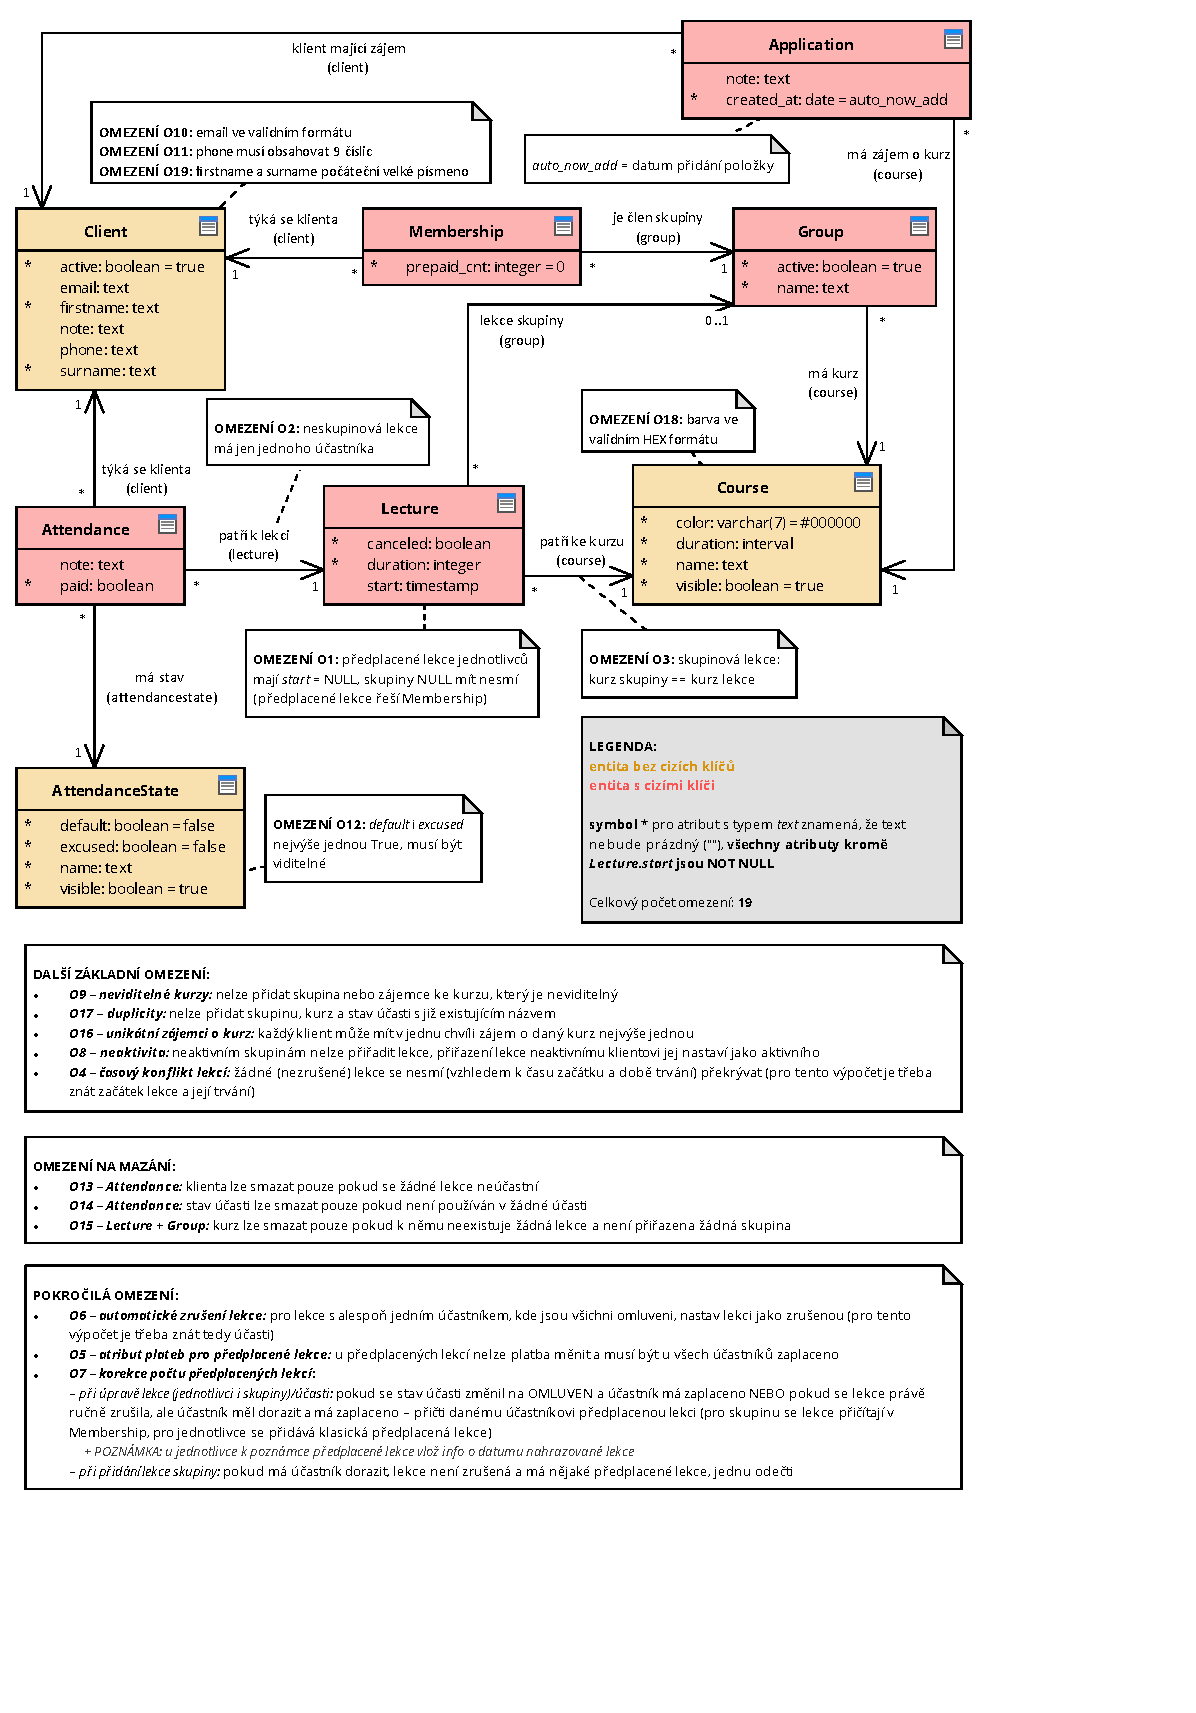
\includegraphics[width=1\textwidth]{img/db-model}
	\caption[Aktualizovaný a rozšířený původní logický datový model]{Aktualizovaný a rozšířený původní logický datový model z~\cite{bp}}\label{fig:db-model}
\vspace{-28pt}
\end{figure}

\subsection{Předplacené lekce}

V předchozím odstavci jsem se dotkl hodnoty \verb|NULL| pro \verb|start| lekce -- zde nastává změna oproti původnímu modelu, protože nyní jsou takto, jak již bylo zmíněno, vedeny pouze předplacené lekce jednotlivců. Díky tomu pak může být u každé předplacené lekce, která se automaticky vytvoří jako náhrada při omluvě/zrušení lekce (viz požadavek~\ref{F10}).

Předplacené lekce skupin jsou pro umožnění jednoduché evidence (viz požadavek~\ref{F3}) nyní součástí členství klientů ve skupině (Membership), tato entita původně byla dekompozicí vztahu M:N bez dalších atributů, prapůvodní záměr v rámci bakalářské práce byl evidování počátku a konce členství klienta ve skupině, což se pak ukázalo jako zbytečné, ale dekompozice byla pro případné jiné budoucí využití ponechána. Nyní tedy konečně dostála svému řádnému využití a umožní tak evidovat počet předplacených lekcí každého klienta v rámci dané skupiny -- když je klient ze skupiny smazán, smaže se samozřejmě i jeho členství a s tím i předplacené skupiny.

\subsection{Zájemci o kurzy}

Dalším funkčním požadavkem~\ref{F1}, který je třeba projevit do datového modelu, jsou zájemci o kurzy. Zde se dá s výhodou jednoduše rozšířit původní datový model o entitu navázanou na klienta a kurz -- tím docílím evidování zájmu klienta o daný kurz (entita Application). Zájem klienta o kurz obsahuje poznámku a také datum přidání, který bude jednoduše automaticky přidávaný, aby lektorka nemusela nic vyplňovat.

\subsection{Vlastnosti stavů účasti}

Požadavek~\ref{F17} uvádí, že je třeba některým stavům přiřadit speciální úlohu -- jeden označit jako výchozí (a zároveň ten, který znamená, že uživatel má přijít/přišel) a druhý jako stav s významem \enquote{klient omluven}. Původní řešení, jak též uvádí \ref{F17}, bylo toto zadefinovat napevno v kódu podle názvu stavu účasti, což je ale nedostačující, protože je samozřejmě třeba tento název umožnit upravit. Nabízelo se několik možností -- zavést nový atribut stavu účasti, který bude označovat typ stavu účasti (jako tomu bývá např. při evidování úrovně oprávnění uživatelů v rámci aplikací). Samotné typy by pak musely být evidovány jako další nová entita. Vzhledem k tomu, že se nepočítá s přidáním dalších typů v budoucnu (stavů účasti také ne, ale ty klidně být přidány mohou, jen nebudou mít speciální typ, protože ten je zde zaveden kvůli dalším speciálním výpočtům jako např. počet absolvovaných lekcí v rámci kurzu), toto řešení nebylo zvoleno z důvodu zbytečné komplexity. Byl zvolen jednodušší způsob, kdy stav účasti má dva boolean atributy \verb|default| a \verb|excused|, kde serverová část obstará, že právě jedna instance stavu účasti bude mít příslušný atribut aktivní. Toto řešení není tak dobře škálovatelné, ale jak jsem uvedl, není to třeba -- je jednoduché a nevyžaduje oproti druhému řešení mnoho změn na úrovni API a klientské části.

\subsection{Další změny}

Aktivita klientů a skupin (viz požadavek~\ref{F6}) se vzhledem k návrhu dá vyřešit jednoduchým atributem \verb|active| u obou těchto entit.

V případě kurzu bylo třeba pro evidování délky trvání kurzu (viz požadavek~\ref{F7}) pro jednotlivce přidat příslušný atribut \verb|duration|. Dalším přidaným atributem je pak \verb|color|, který umožní u kurzu evidovat jeho barvu (viz požadavek~\ref{F12}).

Další změnou, která byla provedena navíc oproti požadavkům bylo přejmenování atributu \verb|name| u klienta na \verb|firstname|. Kromě více vystihujícího názvu (jedná se skutečně o křestní jméno) se zde během vývoje vyskytl problém s nejednoznačností, kde se v rámci klientské části někde pracovalo s \verb|name| jakožto celým jménem klienta, kdežto jinde jako s křestním jménem.

\section{Komunikační rozhraní}\label{sec:komunikacnirozhrani}

Ukázalo se, že původní komunikační rozhraní (REST API) z bakalářské práce mělo velmi dobrý návrh, bylo třeba provést pouze drobnější úpravy a především začlenit všechny potřebné změny z požadavků a datového modelu. Nejprve se zaměřím na drobnější změny a poté na začlenění změn z požadavků a datového modelu. V rámci této kapitoly nebudu uvádět přesnou novou podobu API včetně původních bodů, ale pouze změny, v rámci požadavku~\ref{N1} totiž bude dostupná dokumentace celého API.

\subsection{Opravy a úpravy stávajícího rozhraní}

Pro odpověď na GET požadavek na lekce (GET \verb|lectures/|) byl u každé účasti klienta klíč \verb|count| pro označení pořadového čísla lekce. Zde jsou dva problémy. Prvním je fakt, že název klíče není úplně přesně vypovídající název vzhledem k dané situaci a při práci v kódu nastávaly nedorozumění, proto došlo k přejmenování na \verb|number|, což lépe odpovídá tomu, že se jedná a pořadové číslo lekce. Druhý problém je, že se z neznámého důvodu tento klíč vyskytoval u každé účasti v rámci lekce, což v případě lekce jednotlivce není důležité, ale v případě skupiny je pak totéž číslo u každé účasti (protože se řeší celkový počet lekcí, nikoliv zda konkrétní klient na nějaké lekci byl) -- tedy zbytečně se informace duplikuje a na klientské části se vezme její první výskyt -- toto bylo opraveno a pořadové číslo lekce se nyní vyskytuje přímo u lekce, nikoliv u každé účasti.

Součástí odpovědi GET \verb|lectures/|, jak již bylo zmíněno, je také přehled účastí jednotlivých klientů, zde bylo rozhodnuto také o odstranění vnořených informací o stavech účasti jednotlivých klientů -- v praxi zde byl poslán vždy název účasti, ID (a nově vzhledem k novému datovému modelu by byly poslány i informace \verb|default| a \verb|excused|), vzhledem k plánovaným změnám v rámci požadavku~\ref{N6} tyto vnořené informace byly odstraněny a nahrazeny pouze ID stavu účasti, protože si klientská část aplikace bude stavy účasti pamatovat (díky zavedení React Context API, implementace viz podsekce~\ref{subsec:N6implementace}).

U klientů, jak bylo uvedeno v datovém modelu v předchozí sekci~\ref{sec:datovymodel}, se přejmenoval klíč pro křestní jméno na \verb|firstname|.
    
\newcommand{\apiA}{0.33}
\newcommand{\apiB}{0.14}
\newcommand{\apiC}{0.43}

\subsection{Předplacené lekce}

Pro lepší evidenci předplacených lekcí jednotlivce (viz požadavek~\ref{F3}) bylo třeba umožnit nějakým způsobem na API zaslat požadavek na přidání daného počtu předplacených lekcí. Nejprve byla zvážena možnost vytváření daného počtu lekcí pomocí zaslání POST požadavku na \verb|lectures/prepaid/| obsahujícím příslušný počet předplacených lekcí, vzhledem k jednodušší implementaci a větší univerzálnosti bylo místo toho umožněno zaslat POST požadavek obsahující více různých lekcí (tedy např. i více předplacených lekcí) na \verb|lectures/|.

Pro lepší evidenci předplacených lekcí skupin je na základě předchozí sekce~\ref{sec:datovymodel} zaveden nový bod \verb|memberhips|. V kódu již byl zaveden serializer pro Membership, ten ale nebude použit, protože by pak bod umožňoval upravovat i ID klienta, kterému členství náleží, což zde není třeba -- bude tedy vytvořen druhý serializer pro Membership, který umožní upravit pouze \verb|prepaid_cnt|. Bod pracuje s klíči \verb|id| a \verb|prepaid_cnt| a jeho podoba je následující:

{\centering
\begin{tabular}{p{\apiA\textwidth} p{\apiB\textwidth} p{\apiC\textwidth}}&&\\
    \verb|memberhips/:id/|     & \textbf{PUT}      & úprava členství s \verb|id|\\
    \verb|memberhips/:id/|     & \textbf{PATCH}    & částečná úprava členství s \verb|id|\\
\end{tabular}}

\subsection{Banka}

Přidání úplně nového bodu nastalo kvůli požadavku~\ref{F8} na zobrazení transakcí z banky -- zde API bude nově umožňovat GET na \verb|bank/|, odpověď bude především obsahovat samotná data z banky, která budou dle potřeba transformována (upravena, doplněna, zjednodušena). Pokud by tento bod na API nebyl a klientská část by do banky přistupovala na přímo, znamenalo by to, že nelze provést žádné transformace, zjednodušení dat, přidání dalších dat a také by součástí klientské části musel být token do banky, což je nepřípustné. Lektorka pro ÚP používá bankovní účet u Fio banky, která nabízí zdarma možnost zřízení přístupu k datům účtu přes API, pomocí získaného tokenu je možné každých 30 sekund zaslat na API požadavek \cite{fioapi}. Vzhledem k tomuto časovému omezení (kde by se jinak lektorka při dalším načtení stránky dočkala chybové hlášky) bylo zde rozhodnuto o cachování získaných dat z banky po dobu 60 sekund.

\subsection{Zájemci o kurzy}

Pro evidenci zájemců o klienty byl též vytvořen nový bod, který pracuje s klíči \verb|id|, \verb|note|, \verb|created_at| a dále obsahuje vnořené informace o kurzu (klíč \verb|course|) a klientovi (klíč \verb|client|). Po vzoru ostatních původních bodů se pro úpravy a vytváření zájemců místo vnořených informací zasílá pouze ID a klíč je ve tvaru \verb|klíč_id| -- tedy \verb|client_id| a \verb|course_id|). Podoba bodu je následující:

{\centering
\begin{tabular}{p{\apiA\textwidth}p{\apiB\textwidth}p{\apiC\textwidth}}&&\\
    \verb|applications/|             & \textbf{GET}      & vrátí všechny zájemce\\
    \verb|applications/|             & \textbf{POST}     & vytvoření nového zájemce\\
    \verb|applications/:id/|         & \textbf{GET}      & vrátí zájemce s \verb|id|\\
    \verb|applications/:id/|         & \textbf{PUT}      & úprava zájemce s \verb|id|\\
    \verb|applications/:id/|         & \textbf{PATCH}    & částečná úprava zájemce s \verb|id|\\
    \verb|applications/:id/|         & \textbf{DELETE}   & smazání zájemce s \verb|id|\\
\end{tabular}}

\subsection{Další rozšíření}

Kvůli požadavku~\ref{F6} pro evidenci aktivních a neaktivních klientů byla pro klienty a lekce zavedena možnost filtrování pomocí query string:
\begin{itemize}
    \item \verb|groups/?active=:boolean|,
    \item \verb|clients/?active=:boolean|.
\end{itemize}

V rámci požadavku~\ref{N6} pro optimalizaci API bylo také přidáno filtrování pro kurzy dle viditelnosti -- \verb|courses/?visible=:boolean|.

Do API bylo také třeba projevit změny z datového modelu v předchozí sekci~\ref{sec:datovymodel}. Pro klienty a skupiny přibyl nový klíč \verb|active| znázorňující aktivitu klienta/skupiny. Pro kurzy byl přidán nový klíč \verb|duration| pro evidování délky trvání kurzu a \verb|color| pro evidování barvy kurzu. Stejně tak zde došlo k projevení změn povinných atributů, povolených hodnota ad., vzhledem k použití Django REST Framework ale není v této oblasti na API provádět v kódu žádné změny, protože se projeví automaticky z datové vrstvy (modelů).

Dále, vzhledem ke zvolenému řešení evidování vlastností stavů účasti v předchozí sekci~\ref{sec:datovymodel} je třeba v bodu \verb|attendancestates/| umožnit pracovat nově i s klíči \verb|default| a \verb|excused|, to je velmi jednoduché (proto byl také tento přístup zvolen).

Pro implementaci požadavku~\ref{F9}, který má umožnit jednoduchou automatickou změnu účastníků lekce na klienty, kteří jsou členové skupiny (tedy pokud už např. někdo členem není, tak jej z účastníků odebrat, resp. když byl jako člen přidán a účastník nebyl, tak jej jako účastníka přidat), je třeba umožnit na API toto volitelně učinit. Pro toto je nově zaveden pro bod \verb|lectures/| klíč \verb|refresh_clients| (pro operace PUT, POST, PATCH), výchozí hodnota je \verb|false| (obvykle toto projevení změn účastníků požadováno nebude), při opačné hodnotě pak serverová část zařídí projevení požadovaných změn. 

\section{Architektura}

Aktualizovaný diagram nasazení na obrázku~\ref{fig:deployment-diagram} vychází z původního diagramu \cite{bp}. Jádro zůstává stejné a kromě drobnějších vylepšení pro zlepšení přehlednosti je v něm pouze jedna důležitá změna.
    
\begin{figure}[h]\centering
	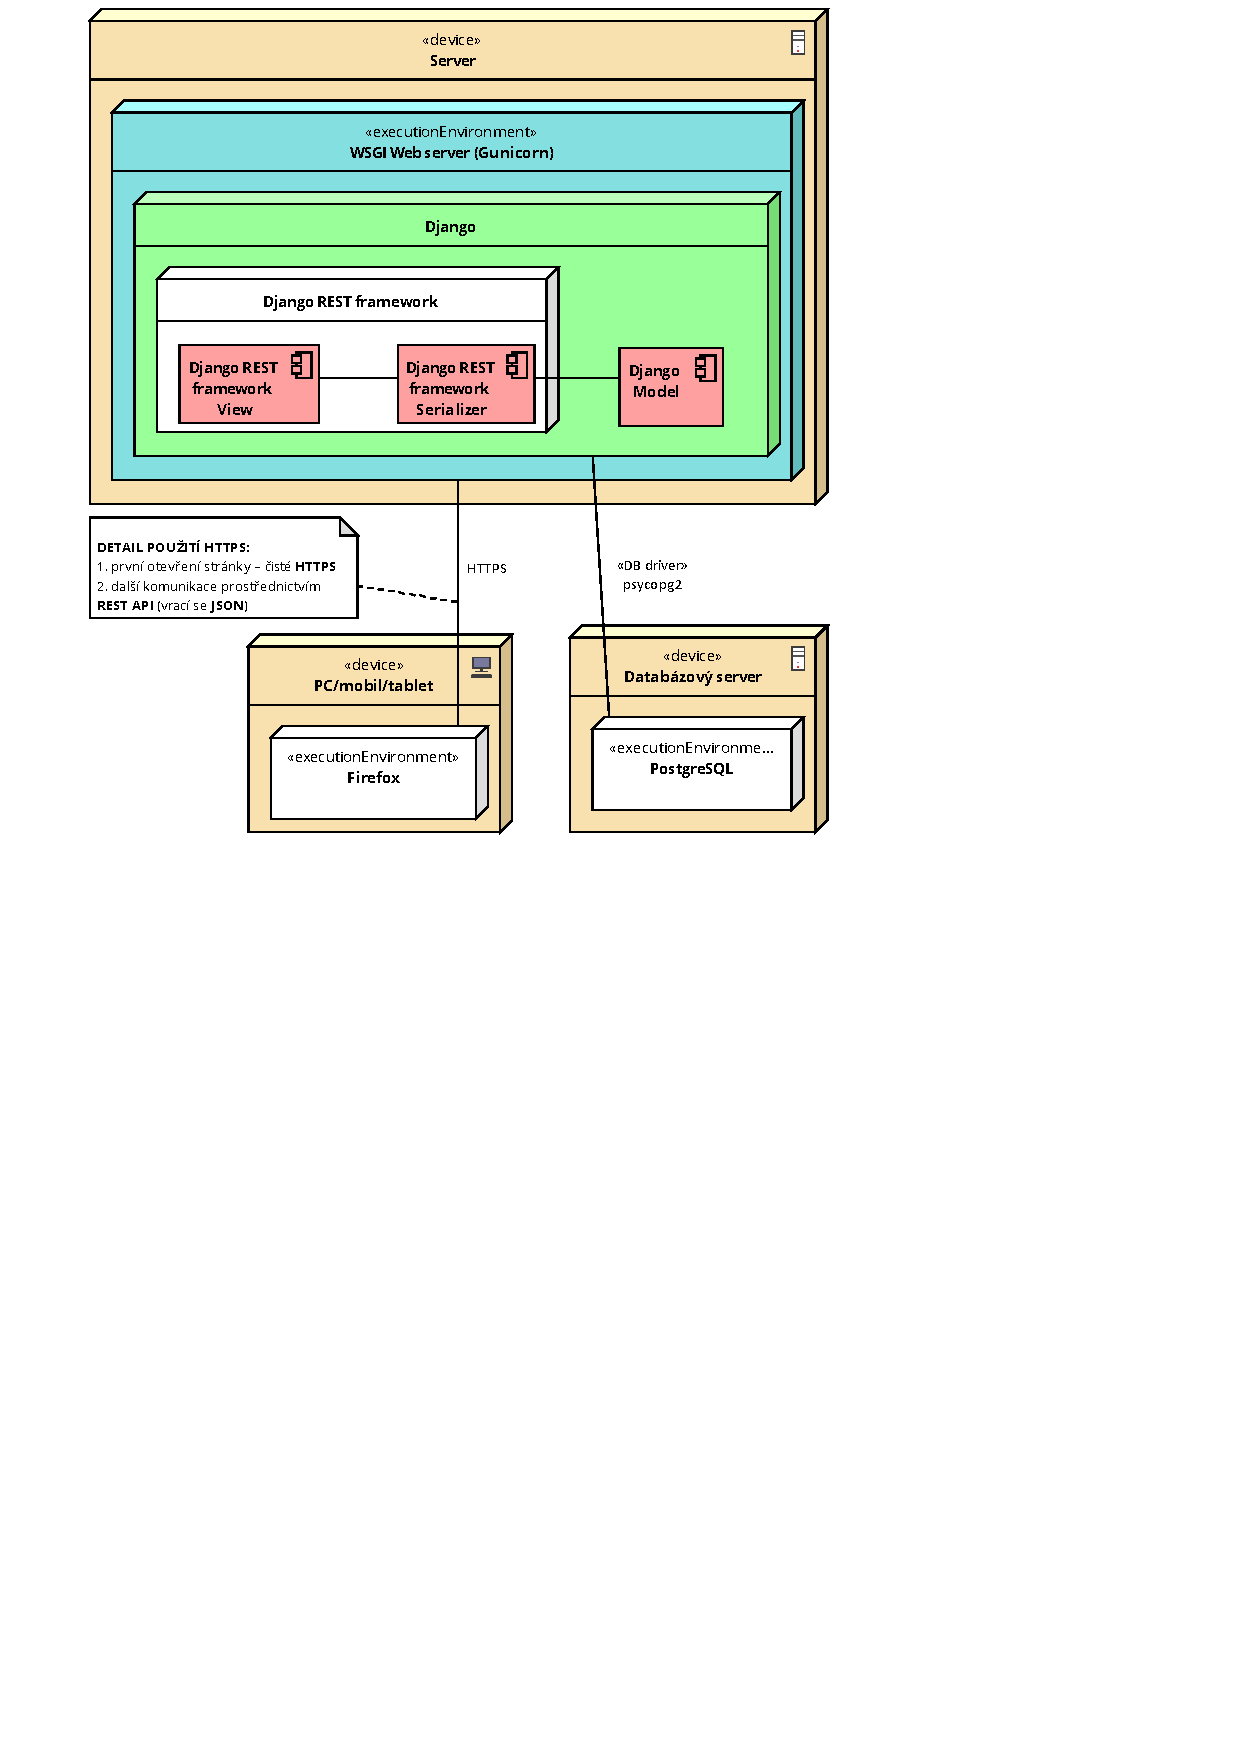
\includegraphics[width=1\textwidth]{img/deployment-diagram}
	\caption[Aktualizovaný diagram nasazení]{Aktualizovaný diagram nasazení, vychází z~\cite{bp}}\label{fig:deployment-diagram}
\end{figure}

V původním diagramu byl jako protokol pro komunikaci mezi serverem a klientem uvedeno HTTP/S. Vzhledem k požadavku na revizi bezpečnosti~\ref{N4} a jeho následné detailní analýze~\ref{subsec:N4detail} je v problému~\ref{B4} zmíněno zavedení HSTS. Podrobnému popisu se budu věnovat v podsekci~\ref{subsec:N4implementace}, důležitý je ale dopad na návrh architektury, kde díky zavedení HSTS a korektní konfiguraci aplikace všechna komunikace bude probíhat z důvodu bezpečnosti pouze přes HTTPS (Hypertext Transfer Protocol Secure).

\section{Konfigurace více prostředí}\label{sec:konfiguraceviceprostredi}

V této sekci se budu zabývat návrhem více prostředí pro nasazování aplikace. Nejprve několik úvodních vět pro uvedení do problému. V současnosti je aplikace nasazena pouze v produkčním prostředí (viz popis aktuálního řešení v sekci~\ref{sec:prostreditestovaninasazovani}), kam se automaticky nasazuje při každém úspěchu na CI. V rámci požadavku~\ref{N7} je uvedeno, že je třeba prostředí totožné s produkcí (např. pro reprodukci chyb) a prostředí s aplikací sestavenou na základě poslední revize v repozitáři.

Jak uvádí \cite{deployment-beanstalk}, více prostředí může jít ruku v ruce se vznikem příslušných větví v repozitáři, jejichž názvy odpovídají prostředím, do kterých se nasazují, probíhají zde slučování změn z jednotlivých větví do jiných a poté nasazování do příslušných prostředí. Vzhledem k tomu, že na aplikaci pracuji pouze já, jedná se o aplikaci na míru pro lektorku a nejedná se o obrovský projekt, tento, ač často užívaný postup, jsem se rozhodl zde nezavést. 

Obvyklý vývoj v repozitáři probíhá pomocí vytvoření nové větve s danou novou funkcí, otestování a začlenění změn do hlavní vývojové větve. Některé menší změny jsou případně prováděny rovnou ve výchozí větvi. Na tomto pracovním postupu jsem tedy vytvořil způsob řešení více prostředí, který bude vhodný pro tento projekt na základě požadavku a všech dosavadních znalostech o projektu.

Byl vytvořen návrh více prostředí bez využití příslušných větví:
\begin{itemize}
    \item \textbf{vývojové (lokální):} pro lokální vývoj,
    \item \textbf{testing:} nasazení každé revize (nehledě na větev),
    \item \textbf{staging:} nasazení pro otagované revize, stejná verze aplikace jako produkce,
    \item \textbf{produkce:} nasazení pro otagované revize, aplikace používaná lektorkou.
\end{itemize}

Jakákoliv nová revize (nezávisle na větvi) v repozitáři bude sestavena a automaticky otestována na integračním serveru a nasazena do prostředí \enquote{testing}. Toto prostředí bude velmi podobné produkčnímu, až na verzi aplikace -- jakékoliv změny v aplikaci po provedení \verb|git push| budou tedy vidět nasazené v reálném prostředí -- bude je zde možné pak testovat manuálně jak mnou, tak lektorkou, řešit další úpravy apod. Zde podotknu, že samozřejmě stále zůstává vývojové (lokální prostředí). Až bude vše vyladěno a připraveno na nasazení do produkce, vydá se nová verze aplikace pomocí tagu v gitu (resp. release v GitHubu) -- pak, když tento otagovaný commit dorazí na CI, proběhnou opět též kroky jako v případě běžného commitu, výsledná aplikace bude ale nasazena nejen do prostředí \enquote{testing}, ale také na \enquote{staging} a produkci. Snažím se zde respektovat obecně známé názvy prostředí (jak třeba uvádí \cite{deployment-beanstalk, deployment-oroinc}). Prostředí \enquote{staging} je přesná kopie produkční verze odlišná pouze svou instancí databáze a slouží např. pro reprodukci problémů hlášených z produkce. Produkční prostředí je verze aplikace používaná lektorkou. Díky zmíněnému návrhu se může na produkci nasazovat až v případě, kdy máme vysokou jistotu hladkého běhu na produkci, tedy například po důkladném automatizovaném i manuálním otestování (v závislosti na změnách). Díky zavedení \enquote{staging} prostředí lze snadno reprodukovat problémy mimo produkci, díky \enquote{testing} prostředí lze okamžitě vidět aktuální změny nasazené v reálném prostředí. Navrženému způsobu dodávání nových verzí aplikace se říká průběžné dodávání (CD -- \enquote{Continuous Delivery}) \cite{deployment-atlassian} a jak uvádí \cite{deployment-atlassian}, pro správné fungování CD je třeba mít dostatečně pokrytou aplikaci testy, což řeší požadavek~\ref{N2}.

\section{Uživatelské prostředí}\label{sec:uzivatelskeprostredi}

Do klientské části bylo třeba navrhnout několik prvků z požadavků. Drobnější změny zde ukázány nebudou, zaměřím se jen na nejdůležitější změny v uživatelském rozhraní. Návrhy obvykle probíhaly na papír, ale pro lepší čitelnost je zde uvádím překreslené v aplikaci \href{https://pencil.evolus.vn/}{Pencil}.

\begin{figure}[h]\centering
    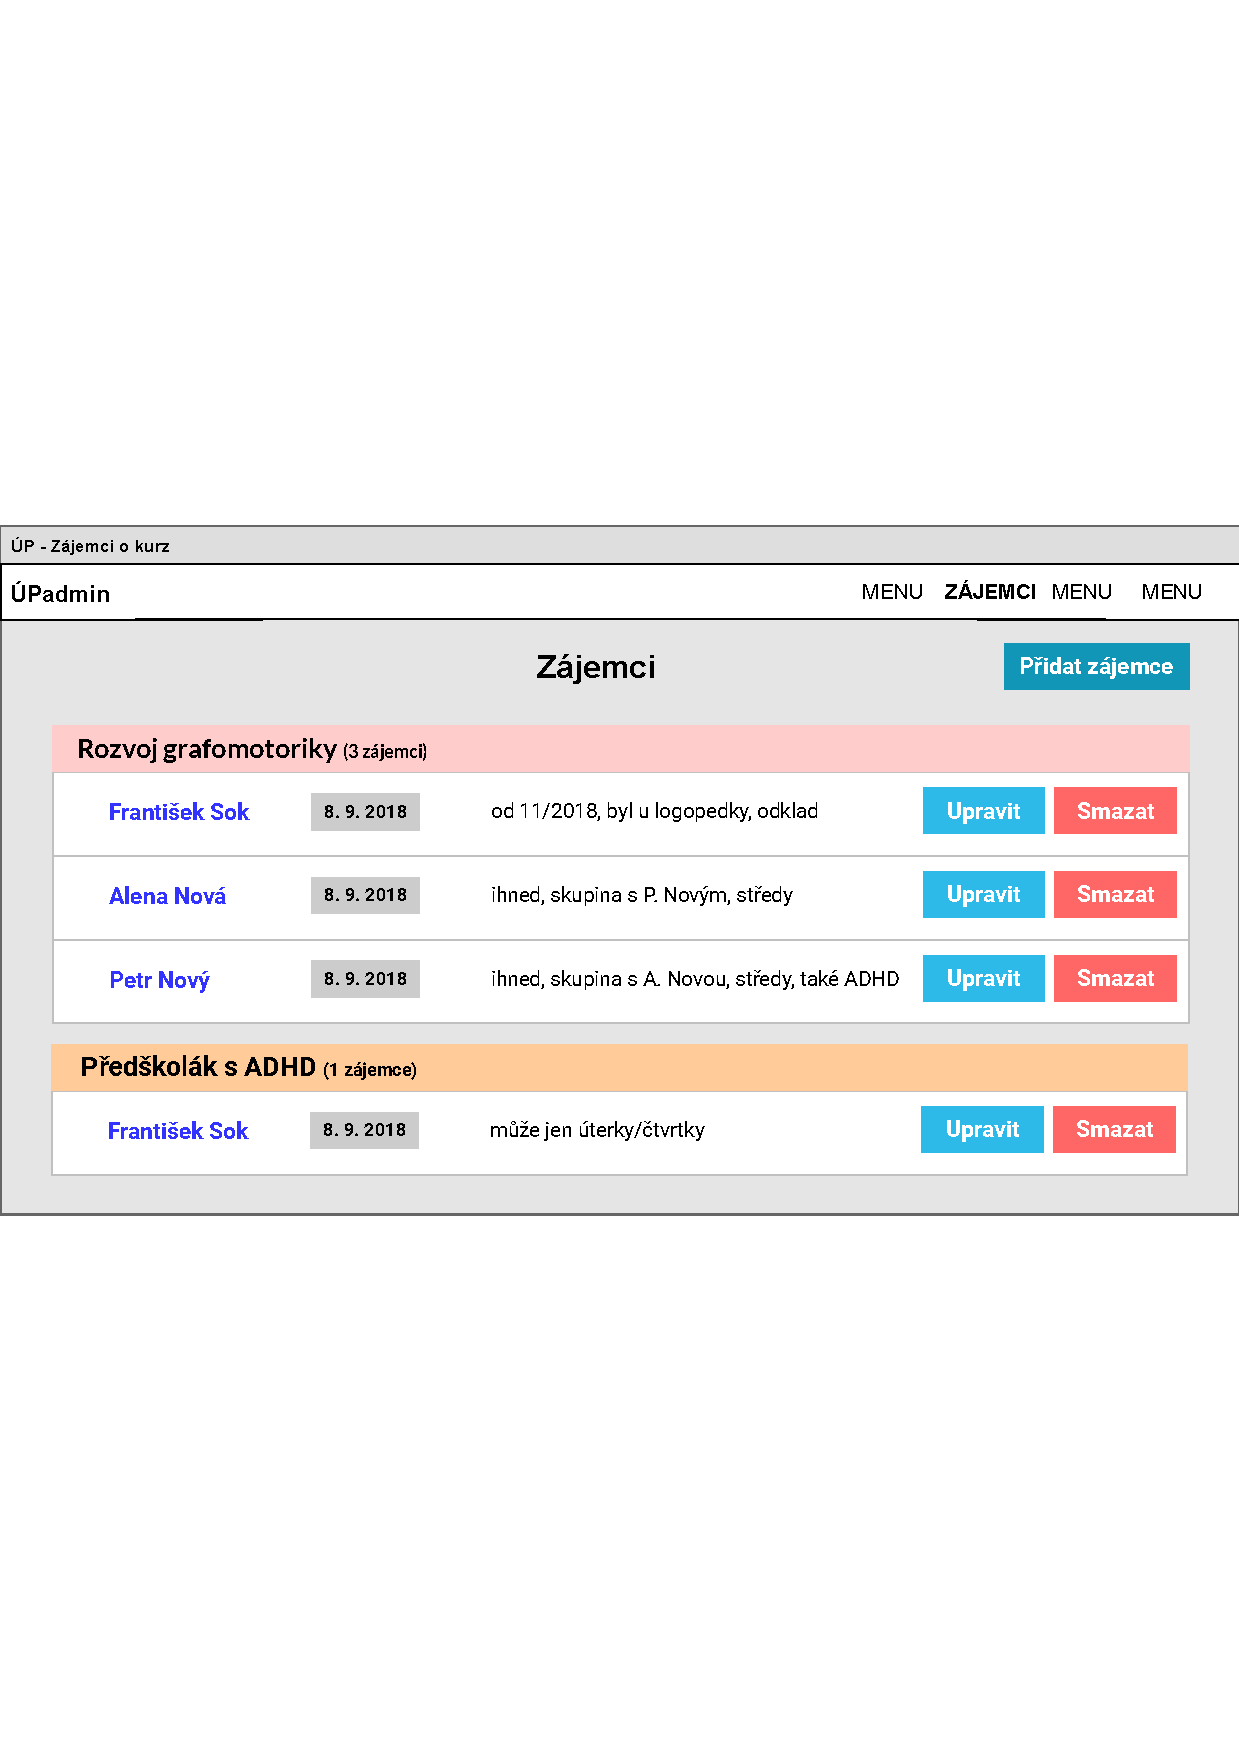
\includegraphics[width=1\textwidth]{img/ui-zajemci}
    \caption{Návrh zájemců o kurzy}\label{fig:ui-zajemci}
\end{figure}

Nejvýraznější změnou v klientské části je přidání nové stránky se zájemci kurzu (viz požadavek~\ref{F1}). Návrh je na obrázku~\ref{fig:ui-zajemci}, jak lze vidět, jsou barevně odlišeny kurzy -- zde již počítám se zavedením požadavku~\ref{F12} pro evidování barev kurzů (změny budou v implementaci učiněny napříč celou aplikací). Návrh splňuje všechny požadavky lektorky, kromě jednoduše dostupné úpravy je také dostupné tlačítko pro smazání -- to je obvykle napříč aplikací dostupné až v modálním okně s úpravou (protože se obvykle stejně nepoužívá a díky tomu, že není přímo na příslušné hlavní stránce, nemůže být ani omylem stisknuto a potvrzeno smazání ve vyskakovacím okně), zde je přímo u každého zájemce, protože oproti ostatním případům zde frekvence mazání bude vysoká vzhledem k postupnému obsluhování všech zájmů o kurzy.

\begin{figure}[h]\centering
    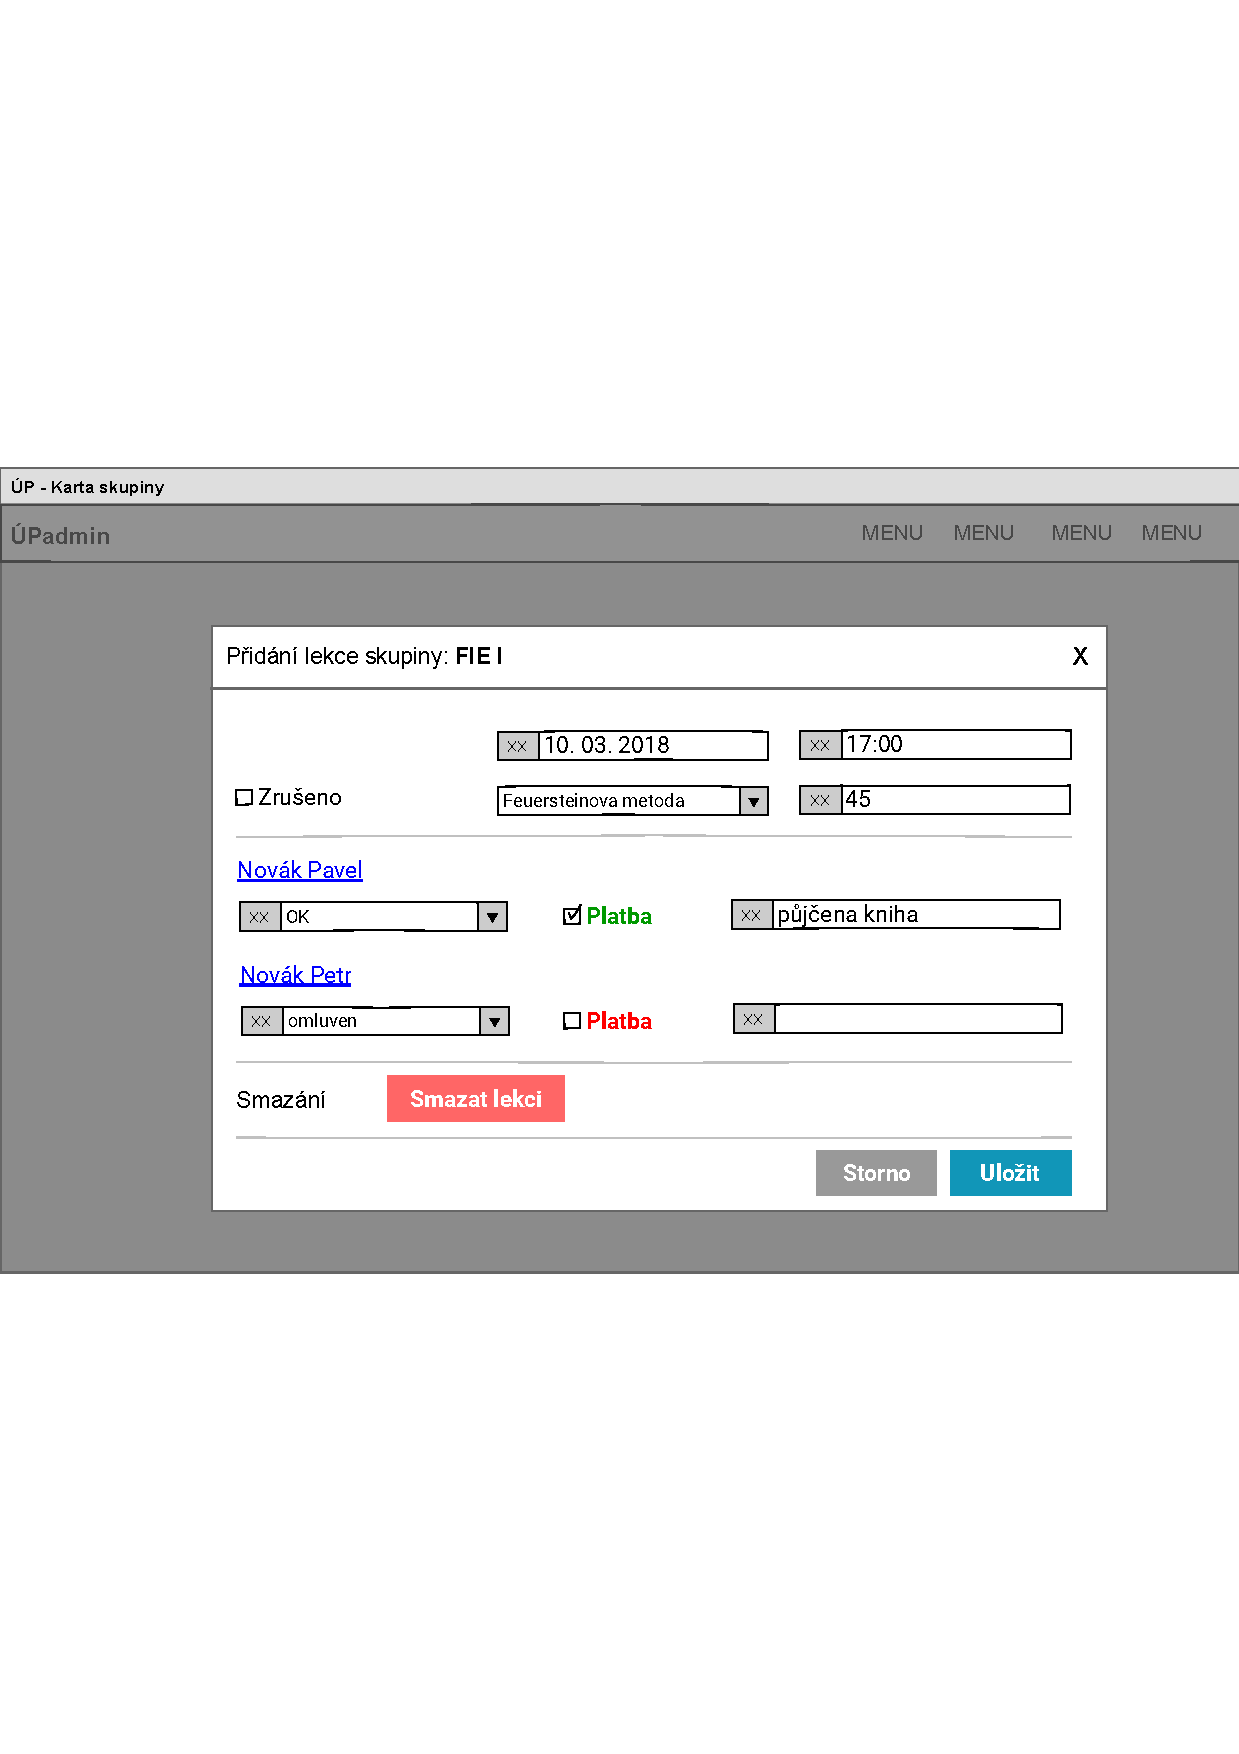
\includegraphics[width=1\textwidth]{img/ui-lekce-skupina}
    \caption{Návrh nového formuláře pro skupinové lekce}\label{fig:ui-lekce-skupina}
\end{figure}

\begin{figure}[ht]\centering
    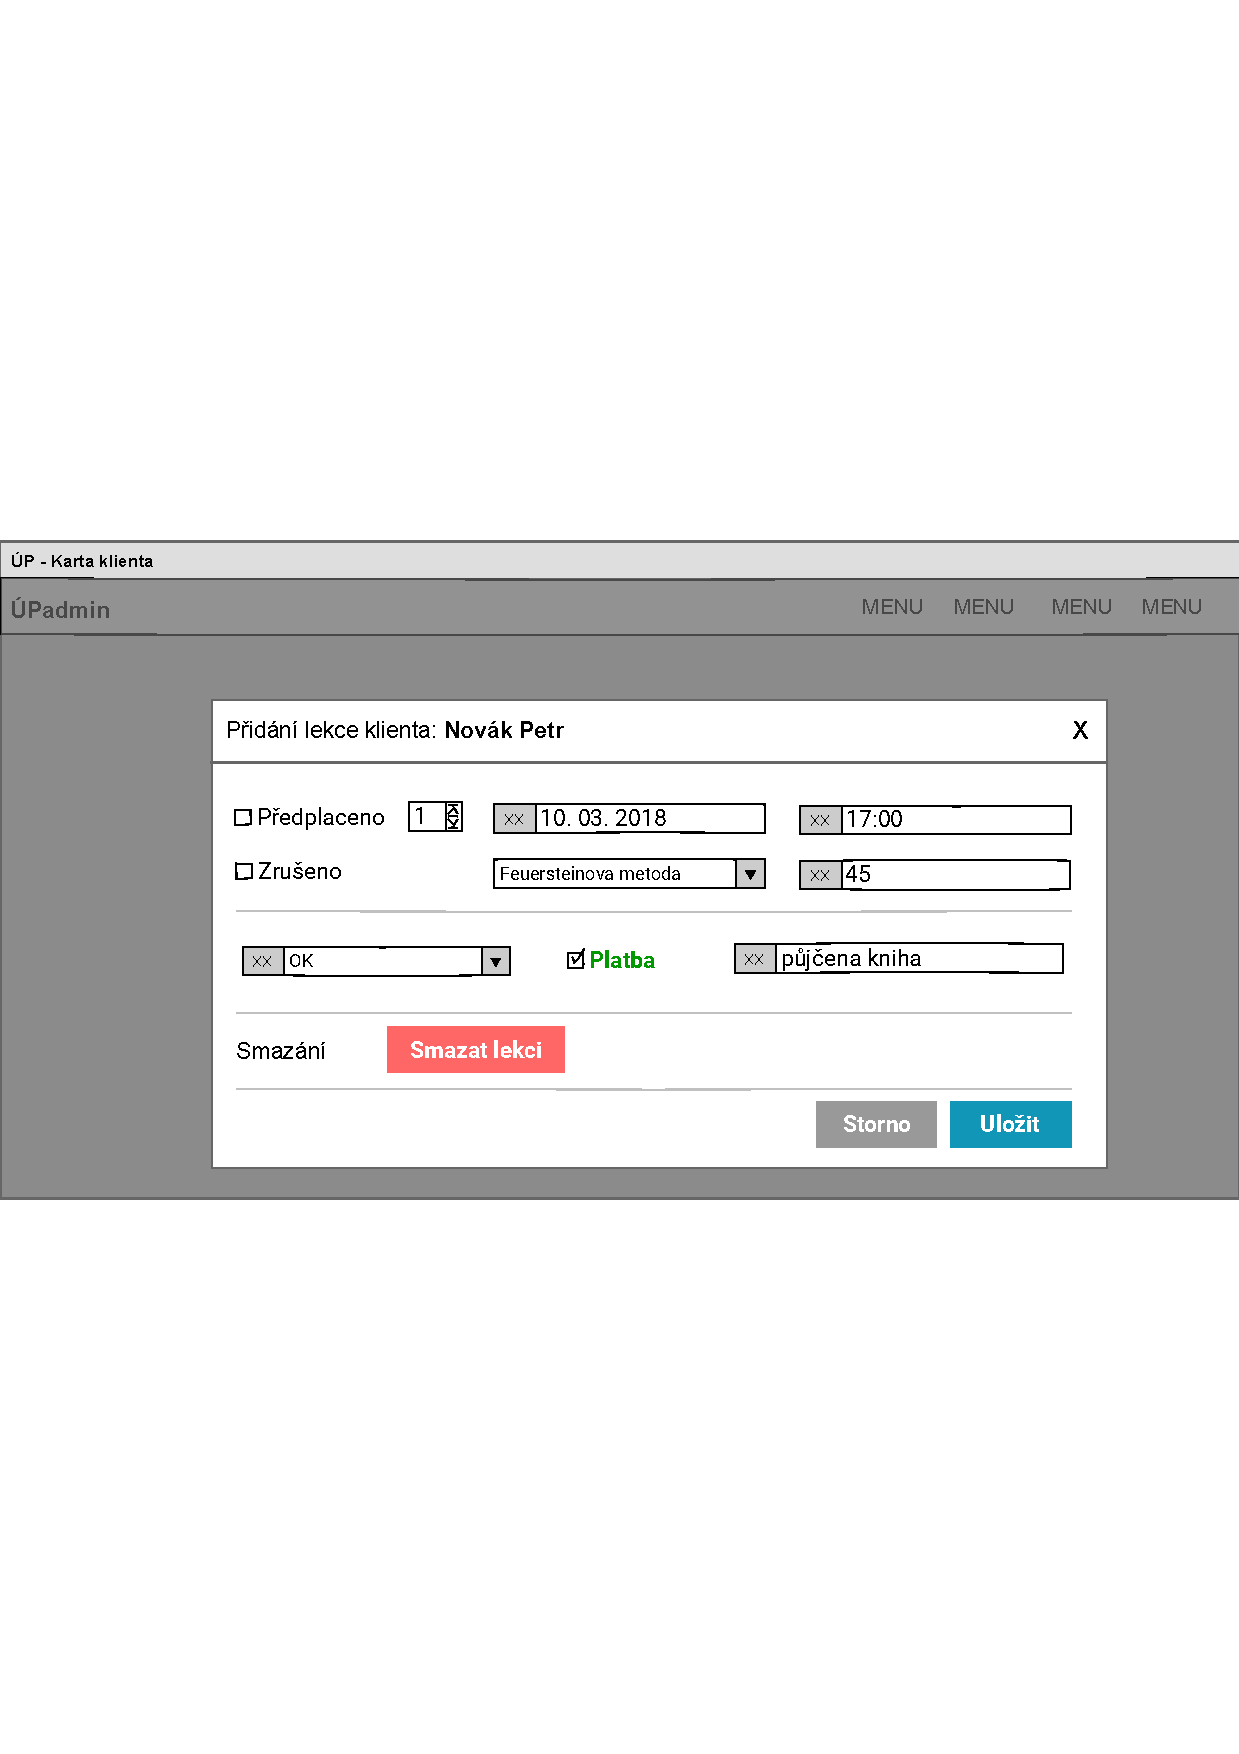
\includegraphics[width=1\textwidth]{img/ui-lekce-klient}
    \caption{Návrh nového formuláře pro lekce jednotlivců}\label{fig:ui-lekce-klient}
\end{figure}

\begin{figure}\centering
    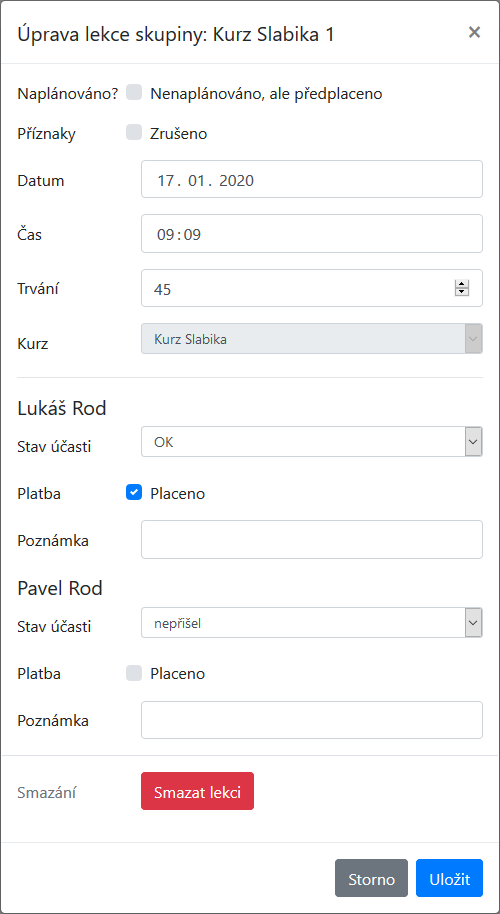
\includegraphics[width=0.55\textwidth]{img/ui-screen-lekce-skupina.png}
    \caption{Původní formulář pro lekce skupin}\label{fig:ui-screen-lekce-skupina}
\end{figure}

Na obrázcích~\ref{fig:ui-lekce-skupina} a \ref{fig:ui-lekce-klient} jsou kompletně přepracované návrhy formulářů pro přidání (a potažmo i úpravu) lekce skupiny, resp. klienta. V rámci příslušného požadavku~\ref{F5} bylo třeba postupnými iteracemi dojít k návrhu, který umožní jednoduší práci s tímto formulářem, který je nejpoužívanější v rámci celé aplikace. V rámci detailní analýzy požadavku~\ref{F3} bylo zjištěno, že je třeba usnadnit přidávání více předplacených lekcí pro jednotlivce, tento požadavek v rámci tohoto přepracování formuláře pro lekce byl též začleněn -- pro klienty je v levém horním rohu dostupné pole pro zapsání počtu předplacených lekcí. Toto pole bude možné upravit při zaškrtnutí volby \enquote{Předplaceno}. Znaky \enquote{XX} u polí naznačují přítomnost ikony vysvětlující význam příslušného pole (místo textů, alternativní text se samozřejmě zobrazí po najetí na ikonu).

Díky větší šířce formuláře bylo možné vměstnat více polí na méně řádků, díky tomu a také ikonám došlo k ušetření místa, díky nově zobrazeným účastem klientů též ve formě řádků, navíc s odlišenou barvou platby je umožněna přehlednější a jednoduší evidence. Jak bylo uvedeno v požadavku~\ref{F5}, jedním z hlavních problémů bylo, že ve skupině může být např. 6 dětí a formulář má pak výšku několika obrazovek a je prakticky nepoužitelný -- zjednodušený názorný příklad původního formuláře (pouze se dvěma účastníky pro jednoduchost, ale účastníků je obvykle mnohem více) je na obrázku~\ref{fig:ui-screen-lekce-skupina}. Formuláře pro skupiny a jednotlivce (klienty) se liší jak počítadlem pro předplacené lekce (u skupin tato možnost není, protože bude řešena počítadly v rámci karty skupiny, viz požadavek~\ref{F3}). Druhou odlišností je pak zobrazení jména účastníka, které v případě jednotlivce je samozřejmě zbytečné (je v horní části formuláře), v případě skupin je toto jméno klienta současně odkazem do jeho karty pro rychlý přechod v případě potřeby.

\chapter{Implementace}

V rámci této kapitoly se budu věnovat způsobu samotné implementace rozšíření aplikace. Nejprve se zaměřím na implementaci funkčních požadavků, poté nefunkčních požadavků a na závěr zmíním další zajímavé problémy řešené během implementace.

\section{Funkční požadavky}

V rámci této sekce popíši způsob implementace všech funkčních požadavků. Pokusím se vždy shrnout jednoduše provedené kroky a také tyto kroky zasadit do kontextu ostatních požadavků a problémů.


\subsection{F1 -- evidování zájemců o kurz}

Pro zájemce o kurzy bylo třeba přidat do serverové části aplikace nový model \verb|Application| (viz datový model v sekci~\ref{sec:datovymodel}), oproti běžným vlastnostem a atributům zde bylo třeba nastavit pomocí parametru \verb|auto_now_add| automatické nastavení data přidání do atributu \verb|created_at|. Na tomto modelu pak staví nově implementovaný bod API pro zájemce (viz komunikační rozhraní v sekci~\ref{sec:komunikacnirozhrani}). Také byly naimplementovány požadované validace a omezení.

Na klientské části jsem vycházel z návrhu uživatelského rozhraní v sekci~\ref{sec:uzivatelskeprostredi}. Bylo třeba přidat do aplikace novou (a v této práci jedinou novou) stránku se zájemci o kurzy a dle návrhu zájemce dělit dle kurzů (API poskytne pouze nerozdělený seznam, tedy toto je třeba řešit na klientské části) a také u každého kurzu dopočíst, kolik je o něj zájemců a zobrazit toto číslo u názvu kurzu (opět dle návrhu). Kurz obsahuje v záhlaví na pozadí svou barvu dle požadavku~\ref{F12}. Důležitou součástí je také formulář pro práci se zájemcem -- ten umožňuje pomocí rozbalovací nabídky \verb|react-select| zvolit jednoduše kurz a klienta (oproti běžnému \verb|select| nabízí možnost vyhledávání a také v případě kurzu zobrazení jeho barvy, viz požadavek~\ref{F12} a související problém s použitelností~\ref{P5}) a připsat ještě poznámku. Taktéž, dle problému~\ref{P7}, jsou zvýrazněny povinné položky. Kromě výběru již existujícího klienta je také možné jedním klikem přidat klienta nového bez opuštění aktuálního formuláře, toto souvisí s požadavkem~\ref{F11} a zároveň opravdu dává smysl, protože většina přidávaných klientů jsou klienti noví, nikoliv stávající -- tedy lektorka by jinak musela formulář zavřít, přejít do klientů, zde klienta vytvořit a poté přejít zpět do zájemců, díky současné implementaci toto ale není třeba a zájemce lze velmi rychle včetně samotného přidání klienta zpracovat v rámci tohoto formuláře pro zájemce.

\subsection{F2 -- kontrola časového konfliktu lekcí}

Kontrola časového konfliktu lekcí má lektorku upozornit ve všech možných případech na překryv dvou lekcí. Existuje mnoho variant, jak se lekce mohou navzájem překrývat, jak ale uvádí \cite{overlap}, lze toto ošetřit jednoduchou podmínkou -- časový konflikt mezi lekcí \enquote{A} a přidávanou lekcí \enquote{B} znamená, že:
\begin{itemize}
    \item \enquote{A} začíná před koncem \enquote{B} a zároveň
    \item \enquote{B} začíná před koncem \enquote{A}.
\end{itemize}

Konec lekce ale v databázi není přímo uložen, známe jen začátek lekce (atribut \verb|start|) a trvání lekce v minutách (atribut \verb|duration|) -- z toho lze ale konec lekce vypočítat. Dotaz na časový konflikt bude tedy mírně složitější a pokročilejší, pro zajímavost finální verzi kódu uvádím v ukázce~\ref{lst:casovekonflikty} (v reálném kódu je tento dotaz rozpadlý do několika částí, pro přehlednost jej zde ale uvádím dohromady), ukázka si vyžaduje samozřejmě vysvětlení.

\begin{listing}[ht]
	\begin{minted}[bgcolor=bg]{python}
qs = Lecture.objects.annotate(
    end_db=ExpressionWrapper(
        F("start") + (timedelta(minutes=1) * F("duration")),
        output_field=DateTimeField()
    )
).filter(
    start__lt=
        data["start"] + timedelta(minutes=data["duration"]),
    end_db__gt=data["start"],
    canceled=False,
)
	\end{minted}
	\caption{Dotaz pro nalezení časových konfliktů}\label{lst:casovekonflikty}
\end{listing}

Dotaz v ukázce~\ref{lst:casovekonflikty} se skládá ze dvou částí -- první část zajišťuje, že se ke všem lekcím dodá atribut \verb|end_db| s dopočítaným koncem lekce, druhá část pak nad těmito lekcemi provede filtrování a nalezne lekce v konfliktu. Nyní podrobněji k první části -- v \verb|annotate| bylo při tvorbě atributu konce lekce \verb|end_db| třeba použít \verb|ExpressionWrapper|, protože typy jednotlivých atributů lekce získaných pomocí výrazu \verb|F()| nejsou stejné, také je třeba číslo uložené v \verb|duration| \enquote{přetypovat} na typ, který zde lze sčítat s typem atributu \verb|start|.

Ve druhé části jsou zakomponovány obě podmínky pro časový konflikt zmíněné výše a navíc se pracuje pouze se zrušenými lekcemi, pro korektní fungování tohoto dotazu je třeba tedy implementovat také požadavek~\ref{F19}. Zde je třeba ještě říci, že lekce, kde jedná končí např. v 15:00 a druhá v 15:00 začíná, nejsou v konfliktu (díky tomu, že se v dotazu neřeší rovnost), což je požadované. Dále je třeba doplnit, že dotaz je dále v reálném kódu ještě ošetřen tak, aby v případě úpravy trvání/startu lekce nebyl hlášen časový konflikt lekce samotné se sebou.

Součástí validace časového konfliktu je také naimplementovaná srozumitelná chybová zpráva pro lektorku obsahující start a dobu trvání lekce a jméno klienta, kterému lekce náleží (případně skupiny)

\subsection{F3 -- vylepšení předplacených lekcí}

Pro pohodlnější evidenci předplacených lekcí bylo třeba na serverové části aplikace upravit model \verb|Membership| (viz datový model v sekci~\ref{sec:datovymodel}) -- doplnit jej o atribut \verb|prepaid_cnt|. Dále bylo třeba tuto změnu projevit i v API (viz komunikační rozhraní v sekci~\ref{sec:komunikacnirozhrani}), stejně jako doplnit do API možnost zaslání více kurzu najednou (pro pohodlnější evidenci více předplacených lekcí jednotlivce), toto řeší v Django REST Framework příslušný \verb|LectureViewSet|, který umožňuje na základě zaslaných dat (jedna lekce/pole lekcí) tyto data zpracovat.

Všechny tyto změny bylo třeba projevit na klientské části -- především dodat pole do formuláře pro přidání lekce jednotlivce, které umožní zadat počet předplacených lekcí (viz návrh UI v sekci~\ref{sec:uzivatelskeprostredi}), tato změna byla součástí kompletního přepracování tohoto formuláře v rámci požadavku~\ref{F5}. Pro evidenci předplacených lekcí pro skupiny, jak bylo uvedeno v analýze tohoto požadavku v podsekci~\ref{subsec:F3detail}, byly do karty skupiny implementována počítadla předplacených lekcí pro jednotlivé klienty. Každý klient má zde hodnotu počtu předplacených lekcí, která lze upravit jak ručně, tak je připravena na automatické projevení změn v počtu předplacených lekcí z požadavku~\ref{F10}. Toto řešení je vidět na obrázku~\ref{fig:ui-screen-pocitadla}. Pokud skupina nemá žádné členy

\begin{figure}[h]\centering
    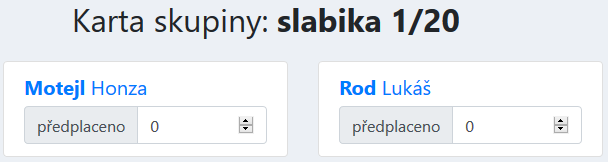
\includegraphics[width=0.8\textwidth]{img/ui-screen-pocitadla.png}
    \caption{Implementace počítadel předplacených lekcí ve skupinách}\label{fig:ui-screen-pocitadla}
\end{figure}

\subsection{F4 -- vyhledávání klientů}

TODO!

\subsection{F5 -- přepracování formuláře pro lekce}

Přepracovaný formulář pro lekce byl implementován dle návrhů na obrázcích~\ref{fig:ui-lekce-skupina} a \ref{fig:ui-lekce-klient}. Součástí implementace byla také migrace z běžné rozbalovací nabídky na \verb|react-select| pro lepší použitelnost a možnost zobrazení barev kurzů (viz požadavek~\ref{F12} a související problém s použitelností~\ref{P5}). Na obrázku~\ref{fig:ui-screen-formular-lekce} je finální implementovaný formulář pro lekce, konkrétně úprava skupinové lekce (od jednotlivce se, jak je též zmíněno v návrhu, liší zobrazením jmen účastníků a naopak nezobrazuje počítadlo předplacených lekcí).

\begin{figure}[h]\centering
    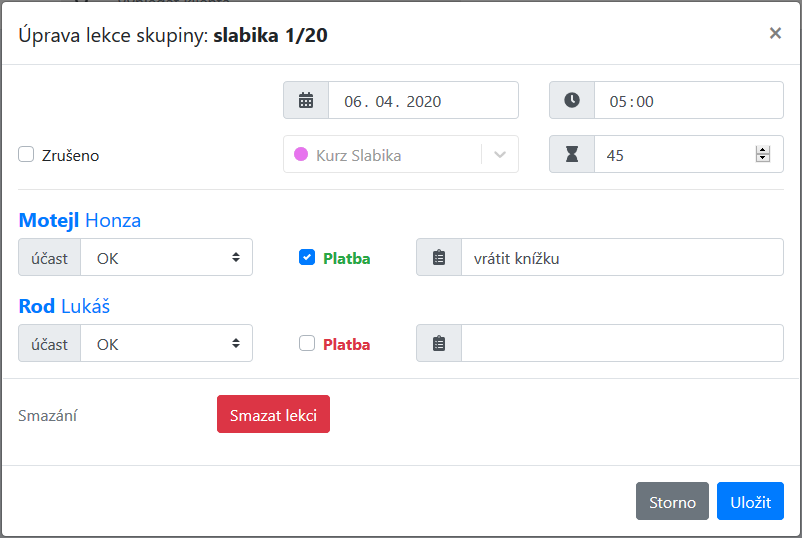
\includegraphics[width=0.9\textwidth]{img/ui-screen-formular-lekce.png}
    \caption{Přepracovaný formulář pro lekce}\label{fig:ui-screen-formular-lekce}
\end{figure}

\subsection{F6 -- zavedení aktivních a neaktivních klientů a skupin}

Pro zavedení aktivních a neaktivních klientů bylo třeba na serverové části aplikace do modelů \verb|Group| a \verb|Client| vložit atribut \verb|active| (viz datový model v sekci~\ref{sec:datovymodel}) a taktéž jej zakomponovat do API (viz komunikační rozhraní v sekci~\ref{sec:komunikacnirozhrani}) -- zde bylo využito propojení modelů s Django REST Frameworkem, tedy do API se změny projeví automaticky. Taktéž byly zavedeny omezení související s aktivitou klientů/skupin, např. při přidání lekce neaktivnímu klientovi se změní na aktivního.

Na klientské části bylo potřeba zvolit, kde se bude z API stahovat seznam všech klientů a kde naopak jen aktivní/neaktivní -- např. při výběru klienta pro přidání lekce stačí stahovat jen aktivní (neaktivním klientům lekce přidat nelze). Dalším důležitým bodem bylo zavést možnost filtrování aktivních a neaktivních klientů/skupin na stránkách se seznamy klientů a skupin. Dle požadavku bylo třeba ve výchozím stavu zobrazit jen aktivní a na vyžádání přepnout do neaktivních. Toto je řešeno komponentou na obrázku~\ref{fig:ui-screen-prepinac-aktivity}. Další implementovanou funkcionalitou nad rámec požadavků pro lepší použitelnost je automatické přepnutí na záložku aktivních/neaktivních klientů/skupin podle toho, do které části patří přidávaný klient/skupina (resp. také upravovaný klient/skupina dle aktivity po uložení).

\begin{figure}[h]\centering
    
\includegraphics[width=0.7\textwidth]{img/ui-screen-prepinac-aktivity.png}
    \caption{Přepínač aktivních a neaktivních klientů}\label{fig:ui-screen-prepinac-aktivity}
\end{figure}

\subsection{F7 -- nastavitelná délka kurzů}

Aby bylo možné nastavit délku kurzů pro jednotlivce, bylo třeba na serverové části aplikace do modelu \verb|Course| vložit atribut \verb|duration| (viz datový model v sekci~\ref{sec:datovymodel}) a opět jej zakomponovat do API (viz komunikační rozhraní v sekci~\ref{sec:komunikacnirozhrani}), což opět automaticky zařídí Django REST Framework.

Na klientské části bylo třeba jak umožnit samotné upravování hodnoty do formuláře s kurzy. Dále bylo ale také potřeba s touto hodnotou vhodně pracovat v rámci formulářů pro vytváření lekce -- tato hodnota totiž, jak uvádí požadavek, platí pouze pro lekce jednotlivců, kdežto lekce skupin mají stále jednu fixní hodnotu. Při automatickém vyplňování hodnoty délky trvání lekce v závislosti na zvoleném kurzu je třeba tedy brát v úvahu, zda se jedná o lekci jednotlivce či skupiny. Na základě toho se pak automaticky vloží daná hodnota do pole pro délku trvání lekce.

\subsection{F8 -- propojení s bankou}

Fio banka, u které má lektorka účet ÚP, poskytuje velmi jednoduchý přístup k API a zde jednoduchý přístup k transakcím -- token se získá v administraci samotného účtu. V datovém modelu aplikace není třeba řešit žádné změny, je třeba ale připravit API pro přístup k transakcím (viz návrh komunikačního rozhraní v sekci~\ref{sec:komunikacnirozhrani}) -- byl vytvořen bod \verb|bank/| umožňující metodou GET získat transakce za poslední 3 týdny. Oproti ostatním bodům, které jsou založeny na datových modelech a používají tak pro vytvoření bodu \verb|ModelViewSet| zde bylo třeba využít obecnější \verb|APIView|, protože s modely nepracujeme. Příslušná metoda \verb|get| je oanotovaná pomocí dekorátoru v ukázce kódu~\ref{lst:cache} -- díky tomu jsou získané výsledky z banky uloženy do cache na 60 s z důvodu omezeného počtu požadavků na API banky (jednou za 30~s).

\begin{listing}[ht]
	\begin{minted}[bgcolor=bg]{python}
@method_decorator(cache_page(60))
	\end{minted}
	\caption{Dekorátor pro zavedení cache}\label{lst:cache}
\end{listing}

Pro použití cache bylo třeba nakonfigurovat Django -- to nabízí mnoho možností ukládání a práce s cache, pro jednoduchost ale bylo zvoleno použití \verb|LocMemCache|, tedy ukládání cache do lokální paměti procesu \cite{django-docs-cache}. V případě pokročilejší práce s cache či pokročilejší aplikace běžící ve více procesech by bylo třeba použít sofistikovanějších možností jako např. databáze Memcached \cite{django-docs-cache}.

Logika práce s bankovním API byla oddělena do samostatného souboru \verb|services.py|, získaná data z banky zde projdou transformací, zjednodušením a doplněním -- odstraní se nepotřebné položky o účtu, doplní se klíč \verb|fetch_timestamp| (timestamp stažených dat z banky, aby bylo jasné, ze kdy získaná data z banky pocházejí), klíč \verb|rent_price| (výše nájmu v Kč), seřadí se transakce od nejnovějších po nejstarší a hodnota zůstatku na účtu se sníží o 100 Kč (minimální zůstatek na Fio účtu, tedy nelze toto započítat do reálně použitelných prostředků, ačkoliv API banky vrátí hodnotu zůstatku včetně této hodnoty). Celá logika je připravena na jakékoliv výskyty chyb ze strany banky, ošetřuje své chování a korektně vrací stavové kódy HTTP. V případě stavových kódů zde bylo otázkou, jak řešit vracení kódu pro požadavky, které zkolabují ze strany API banky, ale ze strany API aplikace proběhnou prakticky korektně, jen neobsahují získaná data -- kód 200 sice dává smysl z hlediska toho, že samotné naše API nemá problém, ale prakticky došlo k interní chybě na serveru, tedy proto zde dojde k vrácení kódu 500 a součástí odpovědi je i přesný popis problému, který nastal.

Na klientské části byla dle požadavku vytvořena komponenta pro napojení na banku umístěná přímo na hlavní stránku do přehledu (zde se tedy nyní kromě přehledu lekcí pro dnešní den nachází přehled transakcí). Lektorka tak už nemusí chodit často do bankovnictví a kontrolovat účet a platby. Součástí této komponenty je i tlačítko umožňující jednoduché znovunačtení dat z banky a také možnost rychle přejít do samotného bankovnictví, pokud je třeba např. zaslat platbu, pokročile vyhledávat či přistoupit k transakcím starších 3 týdnů. Výše nájmu je zde využita k tomu, aby mohla být lektorka případně upozorněna přímo na hlavní stránce na nedostatek prostředků pro uhrazení nájmu na účtu. Zobrazují se dle požadavku transakce za poslední 3 týdny a také aktuální zůstatek na účtu. Součástí přehledu každé transakce je srozumitelný datum (pro blízké dny se také zobrazí např. \enquote{včera}, \enquote{dnes}), částka, barevné rozlišení příchozí a odchozí platby (kromě odlišení znakem \enquote{-}), poznámka k platbě a zpráva pro příjemce. Z analýzy seznamu transakcí banky vyplývá, že v poznámce většiny transakcí se nachází jméno vlastníka účtu, z toho důvodu bylo rozhodnuto v rámci klientské části údaje o transakcích zjednodušit uvedenou formou, tedy zobrazit pouze poznámku (a v případě, že chybí, tak vlastníka účtu) a případně zprávu pro příjemce, je-li uvedena. Transakce z dnešního dne jsou žlutě zvýrazněny dle následného požadavku lektorky. Výsledná komponenta je na obrázku~\ref{fig:ui-screen-banka}.

\begin{figure}[h]\centering
    
\includegraphics[width=0.8\textwidth]{img/ui-screen-banka.png}
    \caption{Komponenta pro informace z banky}\label{fig:ui-screen-banka}
\end{figure}

\subsection{F9 -- změny účastníků skupinových lekcí}

Jak uvádí požadavek~\ref{F9}, je třeba umožnit lektorce jednoduché automatické projevení změn účastníků lekce v závislosti na aktuálních členech. Pro toto bylo třeba dle návrhu komunikačního rozhraní v sekci~\ref{sec:komunikacnirozhrani} zavést nový klíč \verb|refresh_clients| pro operace PUT, PATCH, POST na lekcích.

Tento klíč bylo poté třeba využít na klientské části takovým způsobem, aby si lektorka mohla vybrat, zda chce úpravy/přidání lekce provést bez změn v účastnících, nebo změny automaticky během ukládání provést. Pro toto bylo zvoleno vytvoření druhého tlačítka pro uložení formuláře s popisem \enquote{Uložit + projevit změny v klientech}, po najetí se také zobrazí více vysvětlující popis. Po kliknutí na toto tlačítko dojde jak k uložení změn v lekci, tak k projevení změn v účastnících (po kliknutí na běžné tlačítko \enquote{Uložit} dojde jen k uložení změn).

\begin{figure}[h]\centering
    
\includegraphics[width=0.7\textwidth]{img/ui-screen-formular-projevenizmen.png}
    \caption{Tlačítko pro projevení změn účastníků lekce}\label{fig:ui-screen-formular-projevenizmen}
\end{figure}

\subsection{F10 -- automatické přidání předplacené lekce}

Implementace tohoto požadavku souvisí s požadavkem~\ref{F3} na lepší evidenci předplacených lekcí. Na základě implementace zmíněného požadavku bylo pak možné kód rozšířit a upravit o automatické přidání předplacených lekcí.

Pro jednotlivce bylo naimplementováno, aby se při omluvě klienta/zrušení lekce automaticky klientovi přidala předplacená lekce s poznámkou např. \enquote{Náhrada lekce (7.~4.~2020)}. V případě lekcí skupin bylo využito implementace požadavku~\ref{F3} a klientovi skupiny se předplacená lekce přidá do jeho členství (přičte se k \verb|prepaid_cnt|. V obou případech musely být v kódu přesně stanoveny podmínky, aby došlo k přičtení předplacené lekce právě jednou a nikoliv vícekrát -- například při úpravě již zrušené lekce tedy nesmí být další lekce přičtena.

Součástí požadavku je ale také automatické odebírání předplacených lekcí pro skupiny, což je třeba řešit jak na serverové části, kde dojde k samotnému odečtení předplacených lekcí při přidávání klientů, tak na klientské části, kde při přidávání lekce se automaticky u účastníků označí lekce jako zaplacená v případě, že mají nějaké předplacené lekce. Lektorka tak vůbec nemusí řešit, který klient má danou přidávanou lekci zaplacenou, protože to za ni označí aplikace a po uložení se automaticky odečtou předplacené lekce (pokud klient nějaké má).

\subsection{F11 -- efektivnější práce v rámci aplikace}

V rámci analýzy požadavku~\ref{F11} byl uveden podrobný výčet oblastí, kde je třeba zefektivnit práci v aplikaci -- obecně řečeno se jedná o oblasti, kde je jasné, že je třeba provést určitý úkon a zde pak také vidět výsledky po uložení, ale aplikace toto nenabízí a příslušnou oblast je třeba opustit, provést úkon jinde a manuálně se zpět vrátit do původní oblasti. Problémem je, že původní oblast navíc nemusí být přímo přístupná, nemusí se totiž např. jednat o pouhou stránku s diářem, ale o nějaký formulář, ve kterém je třeba vybrat např. klienta, ale klient zatím není vytvořený -- nejen, že je třeba vše zrušit a přejít do klientů a zde přidat klienta, ale pak je třeba ještě jít zpět na původní formulář, což je skutečně mnoho kroků navíc.

Původní verze aplikace na toto přeužívání formulářů nebyla připravena. Bylo tedy třeba vymyslet takový způsob přeužívání formulářů, že je bude možné využít napříč aplikací bez jakékoliv duplikace kódu a co možná nejjednodušeji.

Řešení přiblížím na konkrétním příkladu -- dle požadavku je třeba umožnit úpravu klienta nejen ze seznamu klientů, ale také z karty klienta. Podívejme se nyní na aktuální situaci v seznamu klientů -- je zde tlačítko pro úpravu klienta, kde po kliknutí lze prostřednictvím formuláře v nově otevřeném modálním okně provádět úpravy. V kódu této stránky je jak příslušné tlačítko, tak i kód obstarávající zobrazení modálního okna, potomkem tohoto modálního okna je uveden pak samotný formulář pro práci s klientem. Jako ideální řešení pro všechny možné situace zadané v požadavcích (tedy i tuto) se ukázalo kompletní odstranění všeho kódu souvisejícího s modálním oknem a formulářem včetně samotných tlačítek. Tento kód byl vždy vyčleněn do speciální komponenty (např. \verb|ModalClients|), která na základě toho, zda obdrží klienta či ne pak zobrazí tlačítko pro přidání, resp. úpravu klienta, které pak otevře formulář pro přidání, resp. úpravu klienta. Na stránce s klienty tedy pouze vložíme komponentu \verb|ModalClients|, které předáme několik potřebných parametrů (tzv. \enquote{props}) a vše ostatní necháme na ní. Tutéž komponentu pak můžeme využít kdekoliv napříč aplikací, stačí ji naimportovat a dát jí potřebné parametry. Všechna logika je obsažena v ní, na jednom centrálním místě. Zmíněný přístup byl použit také pro úpravu skupin v kartě skupiny (původně bylo taktéž možné skupinu upravit jen ze seznamu skupin) a také pro úpravu lekcí jednotlivců i skupin z diáře a přehledu (lekce šly původně upravit pouze v kartě klienta/skupiny). 

Dále bylo třeba vyřešit možnost přidávání klientů např. při vytváření zájemce -- tedy aby lektorka nemusela přidávání zájemce zrušit, přejít do klientů, vytvořit zde klienta, přejít zpět do zájemců a znovu vytvořit zájemce z již založeného klienta. Implementace tohoto je opět založena na komponentách a logice výše, jen je bylo třeba rozšířit o možnost získat z otevřeného formuláře uložená data (např. informace o nově přidaném klientovi), a ty poskytnout jiné komponentě s formulářem (např. formuláři pro zájemce o kurz) -- zde je totiž seznam aktuálních klientů, který my po přidání nového aktualizujeme a rovnou vybereme jako zájemce příslušného nově přidaného klienta. Pro ilustraci je na obrázku~\ref{fig:ui-screen-efektivita-zajemci} vidět, jak je tlačítko pro přidání řešeno -- lektorka je navedena k tomu, že buď zvolí existujícího klienta, nebo když ještě neexistuje, vytvoří nového, a ten se pak, jak již bylo zmíněno, také po přidání automaticky vybere jako zvolený klient ze seznamu již existujících klientů. Totéž řešení je implementováno pro tvorbu skupiny -- tedy lektorka může v klidu vytvářet skupinu a do ní vkládat klienty, které si jednoduše během práce v tomto formuláři s lekcí vytvoří a nemusí jej nikdy opustit.

\begin{figure}[h]\centering
    
\includegraphics[width=0.7\textwidth]{img/ui-screen-efektivita-zajemci.png}
    \caption{Možnost přidat nového klienta přímo při práci v jiném formuláři}\label{fig:ui-screen-efektivita-zajemci}
\end{figure}

Nejtěžším krokem bylo zefektivnění práce s přidáváním lekcí. Je totiž třeba umožnit v diáři i přehledu přidat lekci buď pro jednotlivce nebo pro skupinu. Dále je třeba umožnit rychlé přidání lekce pro daný zobrazený den, ale také pro úplně jiný den, bez jakéhokoliv přecházení na zobrazení tohoto dne (na obrázku~\ref{fig:ui-screen-efektivita-lekce2} je toto vidět -- je otevřená nabídka pro přidání lekce bez určení data, ale vpravo lze vidět možnost přidání lekce pro konkrétní datum). K řešení těchto mnoha cest, kterými se lektorka může chtít vydat, byla vytvořena jednoduchá komponenta \verb|ModalLecturesWizard| (s poměrně složitější implementací), která tvoří prostředníka mezi jakoukoliv stránkou (diář/přehled) a zmíněnými komponentami jako \verb|ModalClients| či \verb|ModalGroups|, které mají na starost práci s formulářem kdekoliv v aplikaci. Tato komponenta může obdržet informaci o dni, pro který se lekce vkládá (když lektorka chce vložit lekci v příslušném dni), ale nemusí (když lektorka chce vložit lekci v jiném dni, který si vybere až ve formuláři pro lekci). Dále, po kliknutí na tlačítko \enquote{+}, které tato komponenta vykresluje, si lektorka zvolí, zda chce přidat lekci pro skupinu nebo jednotlivce (viz obrázek~\ref{fig:ui-screen-efektivita-lekce1}). Poté si (viz obrázek~\ref{fig:ui-screen-efektivita-lekce2}) buď z rozbalovací nabídky zvolí existujícího klienta/skupinu, pro kterou přidává lekci, nebo přidá nového klienta/skupinu (jednoduše bez jakékoliv práce navíc díky napojení na komponenty zmíněné výše, např. \verb|ModalClients|), v obou případech, jakmile dojde k výběru, automaticky se otevře formulář pro přidání lekce skupiny/jednotlivce dle situace s předvyplněným údajem o datu (pokud byl předán komponentě) a mj. také předvyplněnými dalšími informacemi dle požadavku~\ref{F13} (zde je třeba ošetřit případ, abychom např. nepřepsali datum lekce odhadnutým datem následující lekce z implementace tohoto požadavku, protože lektorka již dala jasně najevo, že chce přidat lekci na daný den, nikoliv něco odhadovat). Po uložení lekce dojde k automatickému obnovení původní stránky (diář/přehled) a lektorka vidí všechny změny, aniž by musela za celou dobu někam vůbec přecházet -- vše se dělo v rámci jedné stránky.

\begin{figure}[h]\centering
    
\includegraphics[width=0.7\textwidth]{img/ui-screen-efektivita-lekce1.png}
    \caption{Rychlé přidání lekce -- krok~1}\label{fig:ui-screen-efektivita-lekce1}
\end{figure}

\begin{figure}[h]\centering
    
\includegraphics[width=0.7\textwidth]{img/ui-screen-efektivita-lekce2.png}
    \caption{Rychlé přidání lekce -- krok~2}\label{fig:ui-screen-efektivita-lekce2}
\end{figure}

\subsection{F12 -- evidování barev kurzů}

Bylo třeba implementovat uživatelsky přívětivý způsob výběru barvy kurzů, není samozřejmě možné pouze připravit pole pro zapsání kódu barvy. Zde bylo využito knihovny \href{https://github.com/casesandberg/react-color/}{React Color}, která nabízí množství různých komponent pro jednoduchý výběr barvy -- konkrétní komponenta již integrovaná do aplikace je vidět na obrázku~\ref{fig:ui-screen-barva}. Ve formuláři lektorka jednoduše klikne do pole pro změnu barvy a v této komponentě si barvu vybere. Pro integraci této komponenty bylo třeba vymyslet vhodnou formu otevření a zavření komponenty, v rámci drobného testování použitelnosti na lektorce pak byl finální návrh přijat a nasazen.

Vzhledem k pravidlům použitelnosti a přístupnosti~\cite{wcag} je třeba dbát na to, aby volba konkrétní barvy nezpůsobila nečitelnost jednotlivých komponent v aplikaci -- součástí požadavku je totiž nejen samotná volba barvy kurzu, ale také začlenění této barvy do komponent napříč aplikací pro zvýšení přehlednosti. Zde bylo nejprve třeba napříč aplikací tuto barvu vhodně začlenit všude, kde se zmiňuje kurz -- tedy do přehledu lekcí a diáře, do rozbalovacích nabídek ve formulářích (díky tomu, že jsou řešeny komponentou \verb|react-select| je toto možné), do karty klienta, k seznamu skupin, jichž je klient členem, do seznamu všech skupin. Na základě začlenění barvy do aplikace bylo jasné, že se vždy bude vyskytovat barva kurzu s bílým textem, tedy bylo třeba vyřešit, jak lektorku upozornit, že zvolená barva není příliš kontrastní -- byla vytvořena validační funkce, která díky použití knihovny \href{https://github.com/gka/chroma.js/}{chroma.js} umožní zjistit, na kolik jsou dvě barvy vůči sobě kontrastní a toto porovnat vůči vhodně zvolené konstantě (experimenty bylo zjištěno, že je zbytečně restriktivní vycházet z doporučení WCAG a lze jej mírně zrelaxovat pro možnost volby více barev bez zásadního vlivu na čitelnost). Výsledné začlenění barev napříč aplikací je vidět například na obrázku~\ref{fig:screen-tyden}.

\begin{figure}[h]\centering
    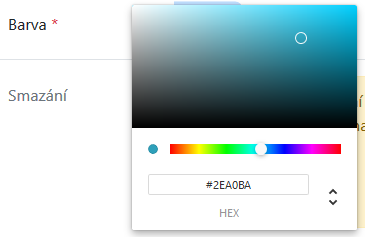
\includegraphics[width=0.6\textwidth]{img/ui-screen-barva.png}
    \caption{Komponenta pro výběr barvy kurzu}\label{fig:ui-screen-barva}
\end{figure}

\subsection{F13 -- automatické předvyplnění údajů lekce}

Dle detailní analýzy~\ref{subsec:F13detail} byly implementovány funkce s daným algoritmem. Funkce jsou oddělené od implementace samotného formuláře i z důvodu požadavku~\ref{F11} pro efektivnější práci v rámci aplikace, kde se počítá s více různými možnostmi přidávání lekcí. Pokud je tedy možné z historie klienta odvodit nové hodnoty pro lekci, při přidávání nové lekce odkudkoliv napříč aplikací se lekce příslušného kurzu (posledního navštíveného) automaticky vytváří o týden později (včetně času) oproti poslední lekci -- tento datum a čas i kurz samozřejmě může lektorka před uložením upravit v případě odlišností, ale ve většině případů bude toto ponecháno bez dalších úprav, protože takto kurzy v mnoha případech fungují. 

\subsection{F14 -- upozornění na ztrátu dat formulářů}

Pro všechny formuláře napříč aplikací bylo třeba implementovat funkcionalitu upozornění na ztrátu nově zadaných dat do formuláře při pokusu o jeho zavření bez uložení. Vzhledem k principu DRY bylo třeba tuto implementaci provést tak, aby byla pouze na jednom místě. K tomu byly využity React Hooks (budu se jim věnovat v sekci~\ref{sec:dalsireseneproblemy}), tedy hook pro modální okno (který poskytuje nejen požadovanou funkcionalitu, ale také sjednocuje práci s modálními okny napříč aplikací) obsahuje indikátor \enquote{dirty}, který při první úpravě lektorkou ve formuláři nabude hodnoty \enquote{true}, v opačném případě (lektorka změny neprovede) nikoliv. Při zavírání jakoukoliv formou (zavření modálního okna či celého okna) se pak provede kontrola indikátoru a případně je lektorka formou vyskakovacího okna upozorněna na ztrátu dat při opuštění, zde může buď jít zpět do formuláře, nebo potvrdit, že o ztrátě ví.

Zde je třeba říci, že z hlediska implementace je odlišné, zda lektorka zavírá jen samotné modální okno s formulářem, nebo rovnou celé okno/panel s aplikací. V případě modálního okna s formulářem se pro zobrazení vyskakovacího okna použije kód v ukázce~\ref{lst:alert1} -- zde se lektorce jednoduše zobrazí okno s textem v kódu. V případě zavření celé stránky se použije kód v ukázce~\ref{lst:alert2} -- zde se přidává naslouchávání na danou událost, kde se při výskytu zavolá daná funkce, ale jak uvádí \cite{mdn-beforeunload}, prohlížeče vyžadují různou podobu této funkce a její chování a také obvykle již nepodporují možnost zobrazit vlastní text zprávy -- funkce byla tedy implementována s důrazem na co nejlepší podporu prohlížečů a lektorce se místo textu v ukázce kódu~\ref{lst:alert1} zobrazí generická zpráva příslušného prohlížeče o možné ztrátě dat.

\begin{listing}[ht]
	\begin{minted}[bgcolor=bg]{javascript}
window.confirm(
    "Opravdu chcete zavřít formulář bez uložení změn?")
	\end{minted}
	\caption{Upozornění na neuložené změny při zavření formuláře}\label{lst:alert1}
\end{listing}

\begin{listing}[ht]
	\begin{minted}[bgcolor=bg]{javascript}
window.addEventListener("beforeunload", beforeUnload)
	\end{minted}
	\caption{Upozornění na neuložené změny při zavření stránky}\label{lst:alert2}
\end{listing}

\subsection{F15 -- vylepšení chybových hlášení}\label{subsec:F15implementace}

Požadavek~\ref{F15} definuje několik částí, na které je třeba se zaměřit. V prvé řadě byl zvýšen časový limit zobrazení chybové notifikace na 15~s (původně nebyl definován, tedy aplikovala se výchozí hodnota knihovny \href{https://github.com/fkhadra/react-toastify}{React-Toastify} 5~s, což nestačilo na pochopení chyby). Všechny chybové hlášky napříč původní aplikací i novými implementovanými požadavky byly revidovány a rozšířeny o více podrobností, možné způsoby řešení -- např. při vzniku časového konfliktu mezi lekcemi je součástí notifikace podrobné info o lekci (datum, čas, klient/skupina, doba trvání) a také info, že je třeba upravit datum a čas lekce. Notifikace také překrývaly menu aplikace, což znesnadňovalo přechod na jiné stránky (bylo třeba notifikací ručně zavřít nebo čekat na automatické zavření) -- notifikace byly posunuty tak, aby menu nepřekrývaly. Notifikace také díky použití nové komponenty \verb|Notification| mají sjednocený vzhled -- obsahují nadpis, ikony symbolizující ne/úspěch a přehledný popis.

Dále bylo třeba se věnovat parsování chyb na klientské části z API. Zde bylo několik problémů -- často se stávalo, že nastala na serverové části chyba, kterou klientská část neuměla rozpoznat a nezobrazila chybu žádnou, lektorka tedy nechápala, proč aplikace \enquote{nic nedělá} (chyba se zobrazila jen v konzoli prohlížeče). Parsování chyb bylo přepracováno a vylepšeno a v případě neznámé chyby se zobrazí také notifikace, stejně tak se lépe a srozumitelněji chyby parsují a je pokryto větší spektrum chyb. Součástí tohoto bylo třeba opravit související problém, kdy při pokusu o smazání entity, která závisí na jiných a je zakázáno ji smazat pokud nějaké tyto závislosti existují (např. smazání klienta s lekcemi), taktéž nedošlo k zobrazení jakékoliv chyby -- zde se ale nehodí obecná chyba a na straně serverové části bylo tedy třeba pomocí kódu v ukázce~\ref{lst:protectederror} toto ošetřit na všech příslušných místech (jednalo se o chybu \verb|ProtectedError|) a dát lektorce srozumitelné vysvětlení, proč se nepodařilo danou entitu smazat.

\begin{listing}[ht]
	\begin{minted}[bgcolor=bg]{python}
def destroy(self, request, *args, **kwargs):
    try:
        result = super().destroy(request, *args, **kwargs)
    except ProtectedError:
        result = super().get_result(
            "Klienta lze smazat jen pokud nemá žádné lekce.")
    return result
	\end{minted}
	\caption{Ošetření chyb při mazání entit}\label{lst:protectederror}
\end{listing}

Jedním z dalších problémů, který nastával, byl pád aplikace na klientské části, který mohl nastat. Takový pád způsobí, že celá aplikace přestane fungovat, zmizí a je třeba celou stránku načíst znovu (toto chování je výchozí od Reactu~16 \cite{react-errorboundaries}, na kterém je tato aplikace postavená). Samozřejmě nejlepší cestou je vše ošetřit, což bylo také učiněno, problémy se ale stále mohou přihodit a je třeba zvolit takové záchranné řešení, aby celá aplikace nespadla a nabídla lektorce možné řešení. React nabízí od verze 16 možnost toto řešit pomocí komponent zvaných \enquote{Error Boundaries} -- je to běžná komponenta, která ale obsahuje navíc jednu (nebo obě) metody \verb|static getDerivedStateFromError| a \verb|componentDidCatch|, tyto komponenty odchytávají všechny chyby ve svých potomcích, logují je a umožňují zobrazit záložní UI \cite{react-errorboundaries}. Je mnoho možností, kam a kolik komponent umístit od zabalení individuálních komponent až po zabalení nejvyšších komponent ve stromu komponent. Zde jsem zvolil přístup zabalení tagu \verb|main| do jedné komponenty zvané přímočaře \verb|ErrorBoundary|, který obsahuje všechny komponenty v rámci aplikace pod menu. Díky tomu při výskytu jakékoliv chyby v těchto potomcích místo pádu a zmizení celé aplikace se zobrazí informace o chybě a stránka je díky zobrazenému menu stále nadále použitelná. Jak bude uvedeno v podsekci~\ref{subsec:N3implementace}, do zmíněné metody \verb|componentDidCatch| bude zakomponováno logování do Sentry a možnost zpětné vazby přiřazené k danému problému.

\subsection{F16 -- titulky stránek}

Každá stránka by měla mít svůj unikátní titulek (zobrazený např. v panelu prohlížeče), v aktuální verzi toto řešeno není a napříč aplikací je jen jeden titulek. Bylo tedy třeba toto zakomponovat do klientské části, konkrétně toto závisí na aktuální stránce, přičemž vzhledem ke SPA architektuře aktuální stránku řeší React Router. Byla tedy implementována komponenta \verb|Page|, kterou React Router vykreslí a ta zároveň zaobaluje samotnou stránku -- jen jí navíc přidá titulek, titulky k jednotlivým stránkám byly přidány formou rozšíření struktury, která doposavad držela pouze URL adresy stránek napříč aplikací.

Toto prvotní řešení, které bylo nasazeno, mělo ovšem jeden nedostatek, který už může být z popisu implementace patrný -- každá stránka (tedy např. karta klienta) má svůj titulek, ale právě jeden. Tedy různí klienti mají stejný titulek na své kartě, tedy \enquote{Karta klienta -- ÚPadmin}. Toto ale není žádoucí, protože při otevření více klientů pak není jasné, který je zobrazený. Totéž platí pro karty skupin a zobrazený týden v diáři. Implementované řešení tedy bylo rozšířeno o možnost manipulovat s titulkem i ze samotné stránky, která je potomkem \verb|Page| -- a to tak, že na základě informací z předka buď má titulek na starost přímo \verb|Page|, nebo jej řeší až její potomek (např. \verb|Card| -- karta klienta) a do titulku vloží např. i jméno klienta, resp. skupiny, resp. pro diář zobrazený týden. Toto je třeba, protože rodičovské komponenty pouze ví, která stránka se bude zobrazovat, neví ale např. jméno klienta (v URL adrese je jeho ID, k němuž si informace získá až potomek \verb|Page|).

Díky tomuto řešení má nyní aplikace např. titulky: \enquote{Novák Dominik – Karta klienta – ÚPadmin}, \enquote{Diář (6. 4. – 10. 4.) – ÚPadmin} a \enquote{Zájemci – ÚPadmin}. Jak je vidět, informace v titulcích jsou řazeny podle důležitosti, tedy v případě prvním uživatel okamžitě vidí celé jméno klienta, pokud by informace byly naopak, viděl by všude nejprve název aplikace a zbytek by neviděl vůbec nebo pouze částečně.

\subsection{F17 -- nastavitelné vlastnosti stavů účasti}

Vzhledem ke zvolenému způsobu řešení evidence vlastností stavů účasti v návrhu datového modelu (sekce~\ref{sec:datovymodel}) bylo třeba dodat do modelu \verb|AttendanceState| atributy \verb|default| a \verb|excused|. Pro oba atributy platí, že hodnotu \verb|true| smí mít vždy nejvýše jeden řádek v databázi. Bylo tedy toto třeba explicitně ošetřit a pro lepší použitelnost byla zakomponována také funkce automatického odznačení příslušného atributu u starého stavu účasti při aktualizaci tohoto atributu -- tedy pokud někdo označí nějaký stav účasti jako stav \verb|excused|, původní stav účasti takto označený je automaticky odznačen. Co se týče komunikačního rozhraní, bylo dle návrhu v sekci~\ref{sec:komunikacnirozhrani} třeba do bodu \verb|attendancestates/| přidat možnost práce s klíči \verb|default| a \verb|excused|.

Na klientské části bylo třeba zvolit vhodný způsob zobrazení informací o tom, které stavy účasti mají jaké označení. Byl zvolen přístup, který jednoduše umožní příslušný stav účasti také změnit (a využije tedy zmíněného automatického odznačení starého stavu) -- v nastavení jsou dvě rozbalovací nabídky, jedna pro stav účasti \enquote{omluven}, jedna pro stav účasti s významem \enquote{dorazil/dorazí} (ten je také výchozí), toto je vidět na obrázku~\ref{fig:ui-screen-vlastnostistavu}. Lektorka zde může snadno změnit příslušný stav, v případě, že je aplikace nasazena do prázdné databáze, jsou zde také zobrazeny upozornění ohledně nenastavených vlastností stavů účastí -- protože v případě, že není ani jeden z atributů u žádného stavu účasti \verb|true|, aplikace nemůže korektně fungovat (resp. funguje, ale např. není schopná korektně spočítat pořadové číslo lekce, automaticky lekce rušit apod.).

\begin{figure}[h]\centering
    
\includegraphics[width=0.7\textwidth]{img/ui-screen-vlastnostistavu.png}
    \caption{Automatické zrušení lekce, když jsou všichni omluveni}\label{fig:ui-screen-vlastnostistavu}
\end{figure}

\subsection{F18 -- omezení a validace hodnot}\label{subsec:F18implementace}

V rámci všech požadavků a také na základě revize stávající domény, jejích entit a omezení byla vytvořena a sepsána v rámci návrhu na obrázku~\ref{fig:db-model}, na základě tohoto návrhu bylo třeba mnoho z omezení doimplementovat -- o některých jsem se již zmínil při implementaci jednotlivých funkčních požadavků. Zde uvedu ještě několik komentářů k implementaci.

Vzhledem k tomu, že počet omezení od původní aplikace poměrně narostl a v čase se i měnil (zde uvádím finální verze návrhu a implementace), bylo třeba, aby byla omezení trasovatelná napříč aplikací a bylo jasné, který kód řeší které omezení -- proto bylo zavedeno značení pomocí identifikátorů (např. \enquote{O13}). Toto označení je pak součástí dokumentace v kódu a implementace je tak prakticky propojená s návrhem, toto řešení tedy kromě trasovatelnosti umožňuje jistou míru konzistentnosti.

Konkrétní implementaci omezení a validaci zde popisovat nebudu, jednak je často zmíněna v textech o implementaci příslušných souvisejících požadavků, druhak se obvykle nejedná o složité konstrukty. Mnoho z validačních metod bylo přesunuto do zvláštního souboru \verb|serializers_helpers.py|, aby byl původní soubor \verb|serializers.py| zachován co možná nejjednodušší. Součástí implementace tohoto požadavku bylo také mnoho ošetření napříč celou aplikací, zejména na serverové části, kde bylo zjištěno mnoho případů, kdy při využití holého API (nikoliv prostřednictvím klientské části) by v datech vznikly nekonzistence a při následném zobrazení na klientské části by mohly být z toho důvodu způsobeny různé problémy. Byly tedy opraveny všechny problémy na API tak, aby pracovalo v souladu s očekáváním a nepovolovalo ukládat do aplikace z pohledu omezení nevalidní data. Mnoho ze zjištěných problémů nebylo odhaleno dříve z důvodu, že klientská část API používá určitým způsobem a mnoha omezeními na klientské části se zamezí už samotnému zaslání nevalidních dat na API -- kdežto při použití čistého API toto někdy hlídáno nebylo.

Do API byly také začleněny některé další transformace dat umožňující konzistentně uložená data, ale s možností zaslání jiného formátu, který je automaticky převeden na požadovaný formát. Příkladem budiž různé délky hexa zápisu barev, mezery v rámci telefonních čísel klientů či velká počáteční písmena křestních jmen a příjmení klientů -- toto řešila klientská část pro lepší použitelnost již při práci v rámci formulářů, pro konzistentnost dat je ale následná validace a transformace kontrolována především také na API. Dalším opraveným problémem byla nefunkčnost některých PATCH metod, které klientská část nepoužívá.

% todo? * zruseni noveho omezeni "neaktivní klienty nelze přiřadit do skupin (UI je ani nezobrazí ve výběru)" - neaktivní klienti již mohou být členové skupiny

\subsection{F19 -- automatické zrušení lekce}

Primární místo, kde se bude řešit automatické zrušení lekce, bude serverová část aplikace -- zde bylo třeba vytvořit funkci, která zjistí dle počtu omluvených účastníků (fakt, že stav účasti znamená omluven lze díky implementaci požadavku~\ref{F17} snadno zjistit) a počtu všech účastníků, zda je třeba lekci zrušit. Funkcionalita byla do funkce oddělena také z toho důvodu, že se zrušení lekce bude řešit nejen při práci s lekcí, ale také při prací se samotnou účastí (\verb|Attendance|) -- např. při rychlé úpravě stavu účasti klienta na lekci bez otevření formuláře se pošle PATCH požadavek na \verb|attendances/:id|, tedy API bod lekcí se zpracováním tohoto požadavku nemá nic společného -- je třeba kontrolu provádět i zde. Funkce byla implementována a korektně fungovala.

Bylo rozhodnuto, že je vhodné, aby se na klientské části (ve formuláři pro lekce) v případě, že jsou všichni klienti lekce omluveni, dávalo najevo, že lekce bude označena jako zrušená. Toto bylo vyřešeno tak, že se pak automaticky zaškrtne \enquote{Zrušeno}, hodnota nelze upravit a vedle se zobrazí symbol s vysvětlením, jak je vidět na obrázku~\ref{fig:ui-screen-automatickezruseni}.

\begin{figure}[h]\centering
    
\includegraphics[width=0.6\textwidth]{img/ui-screen-automatickezruseni.png}
    \caption{Automatické zrušení lekce, když jsou všichni omluveni}\label{fig:ui-screen-automatickezruseni}
\end{figure}

Po nasazení bylo zjištěno, že zde došlo k problému zvoleného řešení tohoto požadavku v souvislosti s požadavkem~\ref{F21}, kdy algoritmus označil jako zrušenou lekci bez účastníků, toto bylo opraveno (viz~\ref{subsec:F21implementace}).

\subsection{F20 -- zobrazení zrušených lekcí}

Vzhledem ke způsobu řešení původního požadavku z bakalářské práce na skrytí zrušených lekcí -- bylo řešeno jednoduchým filtrem na API -- je snadné toto filtrování zrušit a zobrazit tak zrušené lekce i v přehledu a diáři, které právě užívají bod s filtrováním. Filtrování zrušených lekcí bylo tedy v kódu jednoduchou úpravou jednoho řádku zrušeno a zrušené lekce se nyní zobrazují nejen v kartě klientů, ale také se korektně včetně příslušného zvýraznění barvou a symboly zobrazují i v přehledu a diáři.

\subsection{F21 -- skupinové lekce bez účastníků}\label{subsec:F21implementace}

V rámci požadavku~\ref{F21} je zmíněno, že původní aplikace nezvládá evidovat lekce bez účastníků -- serverová část s tímto nepočítá (ale při zaslání lekce bez účastníků neprotestuje), klientská část dokonce při práci se skupinou bez členů a lekcí bez účastníků spadne.

V rámci klientské části bylo třeba opravit chyby způsobující zmíněné pády, dále bylo třeba upravit kód serverové části tak, aby byla na evidování lekcí bez účastníků připravena.

Po opravě chyb se objevil problém, kdy vzhledem k implementaci požadavku~\ref{F19} na automatické zrušení lekce, když nemá nikdo z účastníků dorazit, byly lekce bez účastníků označovány jako zrušené. Toto bylo způsobeno řešením algoritmu, který byl postaven na procházení klientů a srovnávání počtu omluvených s celkovým počtem klientů -- bylo dodáno ošetření, aby lekce bez účastníků nebyly v tomto algoritmu označovány jako zrušené.

\section{Nefunkční požadavky}

V této sekci se zaměřím na implementaci většiny nefunkčních požadavků, některé nefunkční požadavky (\ref{N2}, \ref{N7}, \ref{N8}) budou ale řešeny až v následující kapitolách.

\subsection{N1 -- dokumentace}

Na klientské části (TypeScript) byla do kódu doplněna dokumentace pro všechny exportované funkce a také komponenty (a jejich \enquote{props} a \enquote{state}). V ukázce kódu~\ref{lst:docs-js} je vidět ukázka dokumentace \enquote{props} komponenty \verb|PrepaidCounters|.

\begin{listing}[ht]
	\begin{minted}[bgcolor=bg]{ts}
type Props = {
    /** Pole se členstvími všech klientů. */
    memberships: Array<MembershipType>
    /** Funkce, která se zavolá po aktualizaci
     počtu předplacených lekcí. */
    funcRefreshPrepaidCnt: (
        id: MembershipType["id"],
        prepaidCnt: MembershipType["prepaid_cnt"]
    ) => void
    /** Skupina je aktivní (true). */
    isGroupActive: boolean
}
	\end{minted}
	\caption{Dokumentace v TS (komponenta PrepaidCounters)}\label{lst:docs-js}
\end{listing}

Na serverové části (Python) byla dokumentace dodána ke všem třídám a metodám, mj. obsahuje i popis konkrétních omezení, pokud tato metoda nějaká implementuje -- kvůli trasovatelnosti omezení definovaných v podsekci~\ref{subsec:F18implementace}. Na ukázce kódu~\ref{lst:docs-python} je dokumentace metody pro validování telefonního čísla včetně označení implementovaného omezení.

\begin{listing}[ht]
	\begin{minted}[bgcolor=bg]{python}
def validate_phone(phone: str) -> str:
    """
    OMEZENÍ O11: Ověří, že je telefonní číslo ve správném
     formátu, jinak vyhodí výjimku.
    """
	\end{minted}
	\caption{Dokumentace v Pythonu (metoda pro validaci telefonního čísla)}\label{lst:docs-python}
\end{listing}

Pro dokumentaci API (která v rámci bakalářské práce vůbec nebyla a jediná forma dokumentace byl jednoduchý popis API v tabulkách přímo v textu práce \cite{bp}) bylo využito možností Django REST Frameworku -- ten nově nabízí podporu pro automatické generování OpenAPI schémat (standard pro jazykově nezávislý popis REST API \cite{openapi}), toto vygenerované schéma je pak možné pomocí dalších nástrojů jednoduše zobrazit uživateli srozumitelnou interaktivní formou \cite{drf-openapi}. Díky automatickému generování není třeba nijak aktualizovat dokumentaci API, protože se generuje dynamicky na základě kódu API, pro zobrazení schématu uživateli byl využit nástroj \href{https://swagger.io/tools/swagger-ui/}{Swagger UI}, díky tomu je možné dokumentaci interaktivně procházet a dokonce zasílat na API přímo z UI dotazy (vše je možné pouze po přihlášení). Na obrázku~TODO je vidět ukázka z této dokumentace.

\subsection{N3 -- zavedení nástrojů pro usnadnění vývoje a údržby}\label{subsec:N3implementace}

V této podsekci budu psát o způsobu zavedení nástrojů pro usnadnění vývoje a údržby. V rámci kapitoly~\ref{chap:nastrojeprousnadnenivyvojeaudrzby} byla provedena rešerše možných nástrojů a následně v kapitole~\ref{chap:zvolenetechnologie} bylo zvoleno, které nástroje budou použity, případně vyzkoušeny. Nejprve se zaměřím na zavedení nástrojů pro monitorování chyb a správu logů. Poté popíši způsob zavedení statického typování do serverové části (Python) i klientské části (JS). V poslední části pak popíši způsob zavedení linterů, formatterů a dalších nástrojů pro statickou analýzu kódu.

Pro monitorování chyb bylo třeba zavést nástroj Sentry. Aby bylo možné monitorovat chyby jak ze serverové, tak klientské části, bylo potřeba obě tyto části se Sentry propojit zvlášť. Při výskytu jakékoliv chyby na serverové části se v Sentry objeví podrobné informace včetně kontextu, totéž při výskytu problému na klientské části, kde navíc byla integrována do komponenty \verb|ErrorBoundary| implementované v podsekci~\ref{subsec:F15implementace} možnost zaslání zpětné vazby lektorkou -- tedy při výskytu chyby je možné prostřednictvím formuláře napsat slovy, co se dělo, a tyto informace jsou pak přiřazeny k danému problému v Sentry. Používaný formulář nabízí Sentry, bylo pouze třeba prostřednictvím konfigurace celý formulář přeložit do českého jazyka. Sentry je propojené s Heroku a GitHubem a díky pokročilé konfiguraci v rámci projektu je možné u problémů vidět, ve kterém nasazeném prostředí problém nastal, jaká zde byla verze aplikace, s jakým commitem chyba může souviset apod. Sentry bylo na projektu zavedeno v červenci 2018 a od té doby se ukázalo jako velmi užitečný pomocník, protože díky němu bylo zachyceno a jednoduše reprodukováno mnoho chyb, díky možnosti zobrazit kontext chyby a např. logy z konzole prohlížeče apod. Formulář pro zaslání zpětné vazby lektorka několikrát využila a i díky němu bylo ještě snadnější chyby reprodukovat. Byla analyzována možnost využití nástroje Logentries pro zaznamenávání videa s kroky uživatele, toto zavedeno nebylo -- za prvé díky podrobným informacím ze Sentry a Logentries byl za celou dobu používání vždy k dispozici dostatek informací, za druhé je zde problém s počtem nahraných sezení, kdy se nahrávají všechna sezení, nikoliv pouze ta vedoucí k chybě, tedy snadno se vyčerpá limit 1~000~ nahrávek a až dojde k chybě, nahrávka už nebude.

Pro správu logů bylo třeba zavést nástroj Logentries. Bylo využito možnosti jednoduchého napojení Logentries díky doplňku na Heroku, logy z Heroku jsou tak dostupné v rámci Logentries, je k dispozici historie a vyhledávání. Využito je též upozorňování na některé události, aplikace nabízí ve výchozím stavu mnoho předdefinovaných upozornění. Logentries je na projektu nasazeno od září 2018 a od té doby bylo několikrát úspěšně využito např. pro zjištění historie práce lektorky v rámci aplikace (v rámci reprodukování chyby), díky e-mailovým upozorněním byly včas identifikovány problémy ohledně pomalých operací na API (souvisí s optimalizací API v podsekci~\ref{subsec:N6implementace}) a také byl díky upozorněním odhalen výpadek API Fio banky (kde kvůli nevhodnému ošetření možného výpadku se aplikace nechovala korektně). Prostor pro ukládání logů je dostačující, dle statistik za celou dobu používání bylo nejvíc za měsíc využito 4~MB prostoru.

Napříč celou serverovou částí bylo všude v Pythonu zavedeno statické typování, v ukázce kódu~\ref{lst:statictyping-python} je vidět konkrétní implementace statického typování na kusu kódu. Pro kontrolu typů byla nejprve využita vestavěná typová kontrola v IDE (Pycharm), později byla zavedena i kontrola pomocí nástroje mypy -- díky oběma těmto nástrojům (které mimochodem nemají stejný výstup, po zavedení mypy se objevilo mnoho chyb, na které IDE neupozornilo) bylo nalezeno několik potenciálně problematických míst v kódu, které mohly způsobit různé problémy právě v souvislosti s typy, všechny byly opraveny. Díky zavedení typů tak kromě nalezení několika problémů je k dispozici kompletně oanotovaná základna, což tvoří výbornou dokumentaci kódu. Pro definice typů Djanga a Django REST Frameworku jsou využity \enquote{stubs} \href{https://github.com/typeddjango/djangorestframework-stubs}{djangorestframework-stubs} a \href{https://github.com/typeddjango/django-stubs/}{django-stubs}, po zavedení se ale ukázalo, že definice nejsou úplně kompletní a stoprocentně funkční, bylo tedy třeba na několika místech zavést explicitní ignoraci problémů, protože oba balíčky jsou stále ve vývoji.

\begin{listing}[ht]
	\begin{minted}[bgcolor=bg]{python}
def process_error(self, status_code: int) -> 
    Tuple[Dict[str, str], int]:
	\end{minted}
	\caption{Anotace typů v Pythonu}\label{lst:statictyping-python}
\end{listing}

Pro klientskou část nebylo v rámci kapitoly~\ref{chap:zvolenetechnologie} zvoleno, zda se vydat cestou Flow či TypeScriptu. Vzhledem k tomu, že Flow nabízí vestavěnou integraci pro React (je také z dílny Facebooku), rozhodl jsem se zavést jej jako první a pouze pro část aplikace a na základě následných zkušeností jej buď zavést napříč celou klientskou částí, nebo vše zmigrovat na TS. Během zavádění Flow jsem narazil na mnoho problémů, z nichž většina byla oficiálně nahlášená, ale nijak neřešená -- příkladem budiž naprosto nefunkční integrace s jakýmkoliv IDE/editorem (typová kontrola buď nefunguje, nebo způsobuje zamrzání celého editoru/IDE) a mnoho dalších problémů, které se objeví v průběhu postupného oanotovávání kódu, z nichž většina je hlášená a neřešená. Dalším problémem v průběhu anotování se ukázalo málo typových anotací v databázi flow-typed, pokud definice dostupné byly, často byly chybné a způsobovaly mnoho falešně pozitivních hlášení, které nešly nijak vyřešit, mnoho z nich bylo dlouho hlášených. Potvrdila se tedy zjištění z rešerše v podsekci~\ref{subsec:types-frontend} a vzhledem k tomu, že tedy bylo prakticky nemožné Flow použít kvůli špatné integraci s editory a IDE a mnoha neřešeným problémům bylo rozhodnuto provést kompletní migraci na TS (jako zmíněné firmy a projekty v rešerši).

Vzhledem k tomu, že je v projektu kvůli použití knihovny \href{https://github.com/gaearon/react-hot-loader}{react-hot-loader} potřeba Babel, bylo dle rešerše v podsekci~\ref{subsec:types-frontend} přistoupeno k začlenění TS do projektu pomocí Babelu -- tedy Babel transpiluje bez typové kontroly kód do čistého JS a typovou kontrolu má na starost kompilátor TS propojený s IDE. Integrace s editorem je velmi svižná a nejsou zde žádné problémy jako s Flow. V rámci zavádění TS a anotací se nevyskytl žádný problém, který by byl neřešitelný a třeba jako v případě Flow i hlášený a neřešený. Díky databázi typů DefinitelyTyped je k dispozici mnohem více definicí pro více použitých knihoven v rámci projektu oproti flow-typed a jejich kvalita je vyšší (nedošlo zde k obdobným problémům, jako u Flow -- falešně pozitivní chyby s typy a neřešené problémy). Při anotování jsem narazil na drobné problémy s definicí typů vestavěnou v knihovně \href{https://github.com/FortAwesome/react-fontawesome}{react-fontawesome}, kde nebyl akceptován pro komponentu s ID atribut \verb|id|, ačkoliv v reálu tento atribut použít lze, problém jsem nahlásil a formou PR\footnote{\url{https://github.com/FortAwesome/react-fontawesome/issues/324}} opravil a je již začleněn v nové verzi. Vzhledem k rozsáhlosti kódu zabralo kompletní oanotování typy poměrně dlouhou dobu -- často muselo být totiž zasahováno do kódu, protože byly nalezeny různé problémy právě související s typy a potenciálními chybami. Bylo také třeba důkladně promýšlet a několikrát měnit způsob řešení definicí vlastních typů -- při přípravě a odesílání požadavku na API se například struktura daného typu liší od typu, který z API přijmeme metodou GET, toto všechno muselo být řešeno, definováno, a to tak, aby byly typy snadno znovupoužitelné napříč celou aplikací, rozšiřitelné a srozumitelné. Tyto definované typy entit v rámci klientské části jsou uvedeny v souboru \verb|types/models.ts|, řeší všechny možné případy práce s API (pomocí různých metod a příslušných dat v odpovědích). Postupným zaváděním se přicházelo na více a více drobných i větších problémů ve stávajícím kódu, které byly právě díky explicitním typovým anotacím nalezeny a vyřešeny. Výsledkem práce je kompletní pokrytí celé klientské části anotacemi, převedení všech souborů do TS a zavedení všech souvisejících nástrojů pro TS. Typové anotace jsou maximálně vyčerpávající tak, aby sebemenší chyba v kódu znamenala okamžité hlášení problému ze strany TS kompilátoru. Díky zavedení těchto anotací je také nyní velmi snadné psát kód, protože IDE napovídá vzhledem k typovým anotacím. Příklad části kódu v TS včetně anotací je v ukázce kódu~\ref{lst:statictyping-js}.

\begin{listing}[ht]
	\begin{minted}[bgcolor=bg]{ts}
funcRefreshPrepaidCnt = (
        id: MembershipType["id"],
        prepaidCnt: MembershipType["prepaid_cnt"]
    ): void => {...}
	\end{minted}
	\caption{Anotace typů v TS}\label{lst:statictyping-js}
\end{listing}

Co se týče formatterů, tedy nástrojů pro formátování kódu, na klientské části byl zaveden a nakonfigurován Prettier. Kromě JS, TS a TSX souborů má na starost v tomto projektu také formátování souborů CSS, HTML, JSON, YAML, TOML a MD. Pro Python byl úspěšně zaveden a nakonfigurován Black. Oba nástroje jsou propojeny s IDE a k formátování kódu tak dochází automaticky během práce.

Co se týče linterů (v rešerši v podsekci~\ref{subsec:prubeznakontrolakvalitykodu} bylo zmíněno, že reprezentují prakticky nižší vrstvu nástrojů pro statickou analýzu kódu), byl zaveden a nakonfigurován pro TS nástroj ESLint. Jeho konfigurace v souboru \verb|eslintrc.js| je poměrně rozsáhlá -- kromě konfigurace v souvislosti se samotnými vlastnostmi kódu jej bylo třeba korektně nakonfigurovat pro použití s Reactem, využít pravidla pro kontrolu kódu pro různé oblasti Reactu, dále korektně nakonfigurovat pravidla pro TS, obecná doporučená pravidla ESLint, pravidla, která umožní fungování s formatterem Prettier a mnoho dalších pravidel. V souvislosti se zavedením všech těchto pravidel bylo samozřejmě třeba učinit mnoho oprav a vylepšení v kódu, aby splňoval všechna pravidla. Díky zavedení ESLint je kód klientské části mnohem srozumitelnější, méně náchylný k chybám, přehlednější, konzistentní a bylo opraveno i mnoho problémů (např. překrývání oblastí platnosti proměnných kvůli stejnému názvu, problémy s React Hooky, které mohly způsobit chyby na produkci). Pro CSS byl zaveden a nakonfigurován stylelint, díky jeho zavedení jsou CSS soubory mnohem konzistentnější a přehlednější (např. vlastnosti se řadí dle abecedy) a bylo opraveno také množství různých problémů vycházejících např. z nevhodně definovaných CSS pravidel, duplikace selektorů apod. Pro oba nástroje platí, že mnoho z chyb bylo možné opravit automaticky, čehož bylo také hojně využíváno.

V kapitole~\ref{chap:zvolenetechnologie} o zvolených technologií bylo řečeno, že nalezené nástroje z vyšší vrstvy pro statickou analýzu kódu budou otestovány a následně budou zavedeny ty, které se osvědčí. Vzhledem ke způsobu práce na projektu se ukázalo jako důležité, aby nástroj uměl analyzovat repozitář i bez provedení PR, a to buď přímo v závislosti na commitech, nebo alespoň třeba jednou denně. Proto zde nejsou uvažovány nástroje \href{https://houndci.com}{\textbf{HoundCI}} a \href{https://sider.review}{\textbf{Sider}}.

Výsledky aplikace nástrojů založených na integrací více linterů (nástroje 1.~typu z podsekce~\ref{subsec:prubeznakontrolakvalitykodu}):
\begin{itemize}
    \item \href{https://www.codacy.com}{\textbf{Codacy}}: oproti CodeFactor mnohem pokročilejší rozhraní s více funkcemi, stále ale srozumitelné a přehledné, po aktivaci ESLint se ale ukázalo, že kvůli neaktualizovanému Prettier (na verzi~2) produkuje mnoho falešných chyb, které ale vychází z použití právě nové verze,
    \item \href{https://codeclimate.com}{\textbf{Code Climate}}: velmi podobné možnosti jako Codacy, použité nástroje jsou někdy až o mnoho majoritních verzi pozadu, mohou se tedy objevovat nerelevantní chyby,
    \item \href{https://www.codefactor.io}{\textbf{CodeFactor}}: srozumitelné jednoduché rozhraní, pro ESLint ale nepodporuje soubor s konfigurací ve formátu \enquote{js} (to je pro projekt potřeba), pro stylelint nepodporuje některé závislosti použité jako doplňky (které jsou opět potřeba) -- tedy prakticky neprovádí potřebné kontroly a nelze jej z toho důvodu použít,
    \item \href{https://www.code-inspector.com}{\textbf{Code Inspector}}: velmi nepřívětivé rozhraní působící dojmem nedodělku, často nepřehledné a s chybami (vše je rozpadlé, nefunguje ani tlačítko zpět), nepodporuje ani korektní parsování kódu, protože prakticky každý řádek kódu označí s chybou, nefungují ani importy -- tedy vůbec nefunguje a nelze využít,
    \item \href{https://codebeat.co}{\textbf{codebeat}}: velmi odlišný nástroj, který nenabízí integraci s lintery, pouze základní kontrolu -- nabízí tedy základní upozornění na problémy s kódem jako délka metod, počet argumentů ad., toto zatím v rámci projektu není potřeba.
\end{itemize}

Jak je vidět z výsledků výše, výsledky nejsou nikterak oslňující, kromě základního nástroje codebeat (který ale není třeba) nelze v praxi především kvůli používaní starých verzí nástrojů použít ani jeden z testovaných nástrojů.

Výsledky aplikace nástrojů, které provádějí pokročilou hloubkovou analýzu pomocí vlastních způsobů a pravidel (nástroje 2.~typu z podsekce~\ref{subsec:prubeznakontrolakvalitykodu}):
\begin{itemize}
    \item \href{https://deepsource.io/}{\textbf{DeepSource}}: přehledné a jednoduché rozhraní, zjištěné problémy jsou ovšem spíše základnějšího rázu (který by zvládl podchytit i běžný linter, jak ale bylo uvedeno v rámci kapitoly~\ref{chap:zvolenetechnologie}, linter pro Python zatím není potřeba),
    \item \href{https://deepscan.io}{\textbf{DeepScan}}: velmi jednoduché rozhraní, výhodou tohoto nástroje je úzké zaměření na React a tedy možné odhalení problémů, které jiné nástroje nenaleznou, protože se přímo Reactem nezabývají, v reálu bylo nalezeno jedno možné vylepšení kódu (zjednodušení podmínky), nalezených problémů by pravděpodobně mohlo být více, ale nástroj byl zaveden až po opravení chyb ze všech ostatních nástrojů,
    \item \href{https://lgtm.com}{\textbf{LGTM}}: tento nástroj byl zaveden na projektu jako první a velmi se osvědčil, bylo nalezeno necelých 50 problémů za 10 měsíců vývoje a některé z nich byly poměrně pokročilé a mohly v reálné aplikaci skutečně způsobit problémy (např. špatná práce se stavem v rámci React komponent mohla vzhledem ke svému asynchronnímu principu ve vzácných případech způsobit problémy),
    \item \href{https://sonarcloud.io/}{\textbf{SonarCloud}}: tento nástroj byl na projektu testován jako poslední po všech úpravách hlášených jinými nástroji, přesto v některých souborech odhalil místa pro zlepšení (nikoliv z hlediska přímo problémového kódu, ale zbytečně složitých zápisů, překrývaní oblastí platnosti proměnných, duplikací kódu, jiný název souboru oproti exportované komponentě ad.), také nahlásil několik míst v kódu, které bylo třeba zkontrolovat z hlediska bezpečnosti (protože sám nemůže určit, zda se jedná o problém nebo nikoliv), připomínky byly relevantní, místa byla zkontrolována a nebylo třeba učinit žádné změny (vše bylo v pořádku), nástroj je velmi komplexní a obsahuje obrovské množství pravidel pro různé jazyky a maximální možnou míru konfigurovatelnosti, výhodou je také možnost přímého napojení IDE (Pycharm) a sledování nalezených problémů v reálném čase při psaní kódu, což ostatní nástroje nenabízejí,
    \item \href{https://www.deepcode.ai/}{\textbf{DeepCode}}: nebyly nalezeny žádné chyby ani varování, nelze tedy vyhodnotit, zda to je kvůli slabým schopnostem nebo dobré kvalitě kódu.
\end{itemize}

Nástroje z této oblasti se oproti předcházejícím ukázaly velmi užitečné a díky jejich zavedení bylo nalezeno mnoho různých problémů ať z hlediska srozumitelnosti a udržitelnosti kódu, tak případných chyb na produkci. Zejména se zde osvědčily nástroje LGTM a SonarCloud, navzájem velmi odlišné, ale z hlediska počtu a povahy nahlášených problémů oba velmi užitečné. Pro trvalé zavedení v projektu byly tedy zvoleny LGTM a SonarCloud a dále ještě DeepScan díky svému úzkému zaměření na React. Tyto nástroje trvale sledují změny v repozitáři a upozorní na případné problémy.

\subsection{N4 -- revize bezpečnosti}\label{subsec:N4implementace}

V rámci detailní analýzy tohoto požadavku v podsekci~\ref{subsec:N4detail} bylo vytyčeno celkem 6 oblastí, na které je třeba se zaměřit a vylepšit je. Byly detailně specifikovány problémy, které je třeba opravit. Zde se postupně všem těmto vytyčeným bodům budu věnovat.

Problém~\ref{B1} popisuje problém se zastaralými knihovnami, nerespektováním alespoň drobných oprav v rámci sémantického verzování závislostí, nalezené zranitelnosti v závislostech. Nejprve se zaměřím na serverovou část -- zde byl soubor \verb|requirements.txt|. Pro pokročilou práci se závislostmi, virtuálními prostředími \cite{pipenv-realpython} byl do projektu zaveden nástroj \href{https://pipenv.pypa.io/en/latest/}{Pipenv} a s ním příslušný soubor \verb|Pipfile| obsahující seznam knihoven, na kterých projekt závisí. Všechny verze knihoven jsou zde definovány pomocí \verb|~=| a tedy umožňují drobné aktualizace, všechny knihovny byly aktualizovány na své poslední verze, do kódu a konfigurace aplikace byly projeveny všechny s tím související potřebné změny. Na klientské části se pro správu závislostí používá nástroj Yarn, který byl zachován, bylo ale třeba upravit závislosti v souboru \verb|package.json| tak, aby všechny respektovaly alespoň drobné aktualizace (formou \verb|^verze|). Opět bylo třeba všechny knihovny zaktualizovat na poslední verze a příslušné změny projevit do kódu. Pro klientskou i serverovou část platí, že mnoho z knihoven prošlo poměrně velkými změnami a bylo tedy třeba do kódu samotné aplikace více zasahovat. S aktualizací klientské části souvisí přechod na jiný nástroj pro práci s klientskou částí, o tom bude řeč v sekci~\ref{sec:dalsireseneproblemy}.

Problém~\ref{B2} se sjednocením konfigurací Django aplikace a problém~\ref{B3} ohledně deaktivace \verb|DEBUG| módu Django aplikace spolu souvisejí. Bylo tedy nejprve potřeba kompletně projít lokální a produkční konfiguraci a kde to bylo možné, přesunout konfiguraci z produkční na lokální verzi. Produkční verze totiž importuje všechny konfigurace z té lokální, tedy ji pouze rozšiřuje, není soběstačná. Tím bylo dosaženo toho, že je lokální konfigurace co nejpodobnější té produkční a vyvarujeme se tedy možných chyb, které by se projevily až na produkci. Aby bylo možné na lokálním stroji testovat přímo produkční konfiguraci (tedy např. běh bez webpack-dev-server pouze se statickými soubory), byl v rámci konfigurace aplikace (prostřednictvím proměnné prostředí) zaveden režim \verb|MANUAL_PRODUCTION|, kde lze spustit aplikaci v prakticky totožném prostředí a produkční konfiguraci, jako po nasazení (až na několik drobných výjimek), díky tomu lze ještě přesněji testovat fungování před nasazením. 

V původní verzi aplikace, jak bylo zmíněno v rámci problému~\ref{B3}, byl aktivovaný režim \verb|DEBUG|, jak bylo v rámci analýzy zmíněno, toto není dobře. V rámci inspekce bylo zjištěno, že po deaktivování aplikace přestane na Heroku fungovat, tento problém se do vydání verze pro bakalářskou práci nepodařilo vyřešit. Nyní už byl ale problém zjištěn -- na Heroku se používalo nastavení proměnné pomocí \verb|export|, což ale Heroku nepodporovalo a tedy k nastavení proměnné nedošlo, na tuto proměnnou ale spoléhal následující příkaz \verb|collectstatic|, který sice i tak posbíral všechny statické soubory, ale nikoliv dle produkční, ale dle lokální konfigurace, samotná nasazená aplikace pak běžela v produkční konfiguraci (to bylo v kódu napevno) a soubory nenašla tam, kde měly být. Dotyčná proměnná byla tedy nastavena přímo v Heroku, jak je požadováno, a následně již vše fungovalo v pořádku a \verb|DEBUG| režim se používá jen na lokálním stroji.

Problém~\ref{B4} podrobně popisuje, které HTTP hlavičky v aplikaci v rámci bezpečnosti scházejí -- Referrer Policy, CSP a HSTS. Hlavička \verb|Referrer-Policy| slouží k omezení hodnoty hlavičky \verb|Referer|, která obsahuje informace o předchozí stránce \cite{securityheaders-referer}. Je například nežádoucí, aby se mohly cizí stránky dozvědět, kolik klientů máme v aplikací (díky ID klientů v URL), naproti tomu je ale žádoucí, aby byla někdy známá alespoň doména (např. kvůli povolení zasílání chyb do Sentry v závislosti na jejich původu). Z toho důvodu je v rámci Django konfigurace nastavena tato hlavička na hodnotu \verb|strict-origin-when-cross-origin|, která umožňuje napříč naší aplikací zasílat úplnou adresu (hodí se např. pro Google Analytics, viz zavedení v sekci~\ref{sec:dalsireseneproblemy}), mimo doménu se zašle pouze název původní domény a pokud cílová doména nemá HTTPS, nepošle se nic (proto \verb|strict|). Související problematikou jsou pak odkazy napříč aplikací, které se otevírají v novém panelu (\verb|target="_blank"|) -- zde se může vyskytnout útok na původní stránku, odkud došlo k otevření \cite{noopener}, proto bylo do takovýchto odkazů dodán atribut \verb|rel="noopener noreferrer"| -- dokonce v některých případech (bankovnictví Fio) se bez tohoto atributu nedá v nově otevřeném panelu zobrazit přihlašovací formulář, stránka místo toho zahlásí, že došlo k úspěšnému odhlášení.

Hlavička \verb|Strict-Transport-Security| umožňuje, aby prohlížeč komunikoval se serverem už od počátku přes HTTPS, jinak jsou první komunikace jen v HTTP, což umožňuje útok typu \enquote{man-in-the-middle} \cite{securityheaders-hsts}. Díky možnosti registrace stránky do autoritativní databáze na adrese \href{https://hstspreload.org/}{https://hstspreload.org/}, která je distribuována do jednotlivých prohlížečů, lze i při úplně první komunikaci s webem (a pak i dalších prvních komunikacích) fungovat přímo přes HTTPS \cite{jakpsatweb-hsts}. Django konfigurace opět umožňuje nastavit HSTS, konkrétní nastavení je v ukázce kódu~\ref{lst:hsts}.

Hlavička \verb|Content-Security-Policy| určuje prohlížeči, odkud může které zdroje načítat -- díky tomu nabízí prevenci např. vůči XSS (Cross-Site Scripting) útokům \cite{adamj}. Django nenabízí nativní podporu CSP \cite{adamj}, k tomu byla využita knihovna \href{https://django-csp.readthedocs.io/en/latest/}{django-csp}. Obsah této hlavičky může být poměrně pokročilý a rozsáhlý vzhledem k počtu nabízených možností \cite{adamj} -- proto zde její finální verzi nebudu ani uvádět. Při její tvorbě bylo třeba upravit práci s některými knihovnami a nástroji tak, aby nevkládaly JS/CSS kód přímo do stránky, ale zvlášť do souborů, dále bylo třeba umožnit aplikaci komunikovat se Sentry, Google Analytics, Google Fonts a umožnit správné fungování všech částí aplikace, protože v původním stavu by aplikace nefungovala vůbec. Na základě dalších doporučení např. z \cite{dareboost} či přímo nástroje \href{https://observatory.mozilla.org/}{Mozilla Observatory} (který na chybějící CSP hlavičku v~\ref{subsec:N4detail} upozornil) byla hlavička rozšířena o další hodnoty až do své finální verze, kdy je kompletní a nástroj Mozilla Observatory ji hodnotí stupněm \enquote{A+} se skóre 115/100.

\begin{listing}[ht]
	\begin{minted}[bgcolor=bg]{python}
SECURE_HSTS_SECONDS = 63072000  # 2 roky
SECURE_HSTS_PRELOAD = True
SECURE_HSTS_INCLUDE_SUBDOMAINS = True
	\end{minted}
	\caption{HSTS konfigurace}\label{lst:hsts}
\end{listing}

V rámci~\ref{B5} je třeba zavést jednotnou práci s proměnnými prostředí napříč aplikací. K tomu byla použita knihovna \href{https://django-environ.readthedocs.io/en/latest/}{Django-environ}, která umožňuje proměnné prostředí převést na odpovídající typy pro použití v Pythonu (např. řetězec \verb|True| se převede na boolean s hodnotou \verb|True|) a také umožňuje proměnné prostředí naplnit hodnotami ze souboru \verb|.env| \cite{django-environ}. Těchto funkcí bylo využito tak, že na lokálním stroji jsou hodnoty proměnných prostředí uloženy ve zmíněném souboru, při spuštění aplikace jsou načteny do proměnných prostředí a mohou být využívány. Při nasazení se pak již nevyužívá tohoto souboru, ale proměnné prostředí jsou definovány přímo na Heroku prostřednictvím GUI/CLI aplikace (Command Line Interface) a jejich rozparsované hodnoty se pak taktéž používají v rámci aplikace. Další výhodou tohoto řešení je možnost nastavit výchozí hodnoty pro různé proměnné prostředí. Celkem bylo takto zavedeno 11~proměnných prostředí, mj. sloužících pro uložení údajů pro přístup do databáze, dalších tokenů a také proměnných indikujících určité stavy aplikace (např. zda je aktivováno bankovnictví ad.). Díky tomuto přístupu také bude jednoduché zprovoznit v rámci požadavku~\ref{N7} více různých prostředí pro nasazení a také umožnit jednoduché zprovoznění aplikace u kohokoliv (což je výhodné v souvislosti s plánem vystavení aplikace jako open-source). Ukázka konfigurace proměnných prostředí v rámci knihovny Django-environ (v konfiguraci Djanga) je vidět v ukázce kódu~\ref{lst:envvars} (proměnné nejsou uvedeny všechny).

\begin{listing}[ht]
	\begin{minted}[bgcolor=bg]{python}
env = environ.Env(
    DATABASE_URL=str,  # url pouzivane DB
    SECRET_KEY=str,  # tajny klic pro Django
    FIO_API_KEY=(str, ""),  # token pro pristup do Fia
    BANK_ACTIVE=(bool, True),  # aktivace propojeni s bankou
    ...
)
	\end{minted}
	\caption{Ukázka konfigurace proměnných prostředí}\label{lst:envvars}
\end{listing}

Problém~\ref{B6} popisuje požadavek na zakázání indexování všem robotům. Zde je volba mezi několika způsoby -- zákazem procházení prostřednictvím souboru \verb|robots.txt| a zákazem indexování pomocí \verb|meta| tagu (případně HTTP hlavičky \verb|X-Robots-Tag|) \cite{roboti}. Soubor \verb|robots.txt| sice zakáže procházení stránky roboty, stránka ale stále může být zaindexována z jiné stránky, z toho důvodu je zvolena druhá možnost, která nezakáže procházení, ale zakáže indexování ve všech případech, řešení je v ukázce kódu~\ref{lst:robots} -- důležitý je zde především parametr \verb|noindex|, který toto řeší. 

\begin{listing}[ht]
	\begin{minted}[bgcolor=bg]{html}
<meta name="robots" content="noindex, nofollow"/>
	\end{minted}
	\caption{Kód pro zákaz indexování webu vyhledávači}\label{lst:robots}
\end{listing}

\subsection{N5 -- vylepšení použitelnosti}

V rámci detailní analýzy požadavku~\ref{N5} v podsekci~\ref{subsec:N5detail} bylo zjištěno celkem 20~problémů s použitelností. V této sekci popíši některá řešení těchto problémů -- především ta zajímavější. Řešení některých problémů zde naopak popisovat nebudu, protože není příliš zajímavé (ale všechny byly vyřešeny) -- řešit zde nebudu problémy \ref{P3}, \ref{P4}, \ref{P6}, \ref{P8}, \ref{P9}, \ref{P10}, \ref{P12}, \ref{P14}, \ref{P16}, \ref{P18} a \ref{P20}.
 
\textbf{\ref{P1}:} Lektorka nebyla nijak informována o délce načítání -- byla rozšířena komponenta \verb|Loading| mající na starost zobrazení informace o načítání o informování vzhledem k času, tedy po 5~sekundách se lektorce navíc zobrazí informace, že aplikace stále pracuje a načítá, po 25~s (což je dostatečně dlouhá doba na to, aby se případně i probudila aplikace na Heroku, pokud spí v rámci programu zdarma) se zobrazí výstražnější upozornění, že pravděpodobně došlo k nějaké chybě a je třeba aplikaci načíst znovu (včetně tlačítka pro načtení znovu), toto je vidět na obrázku~\ref{fig:ui-screen-loading}.

\begin{figure}[h]\centering
    
\includegraphics[width=0.9\textwidth]{img/ui-screen-loading.png}
    \caption{Upozornění při velmi dlouhém načítání}\label{fig:ui-screen-loading}
\end{figure}

\textbf{\ref{P2}:} Chyběly popisy u některých netextových prvků, případně byly formou \verb|title|, kterou nelze zobrazit na dotykových zařízeních. Toto bylo vyřešeno jak dodáním a vylepšením samotných popisů, tak využitím komponenty \verb|Tooltip| z knihovny Reactstrap, která umožňuje zobrazit lépe čitelné popisy, které lze navíc otevřít i na dotykových zařízeních. Zde byl při implementaci objeven v knihovně Reactstrap problém, který na iOS způsoboval, že se popis zobrazil vždy až po druhém kliknutí, problém byl nahlášen a poté jsem jej formou PR do tohoto repozitáře\footnote{\url{https://github.com/reactstrap/reactstrap/issues/1676}} opravil, oprava je již vydána v nové verzi.

\textbf{\ref{P5}:} Některé prvky pro rozbalovací seznamy nebyly řešeny uživatelsky přívětivým \verb|react-select| -- kde tedy bylo třeba dle analýzy, byly tyto seznamy nahrazeny \verb|react-select|, na obrázku~\ref{fig:ui-screen-select} je vidět, jak tyto komponenty mohou práci usnadnit -- umožňují např. vyhledávat, dodat barvy ke kurzům (a v případě členů skupiny umožnit výběr více položek, tedy klientů, naráz).

\begin{figure}[h]\centering
    
\includegraphics[width=0.4\textwidth]{img/ui-screen-select.png}
    \caption{Komponenta react-select pro výběr kurzů}\label{fig:ui-screen-select}
\end{figure}

\textbf{\ref{P7}:} Napříč aplikací nebylo poznat před odesláním formuláře, která pole jsou povinná. Toto bylo napraveno dodáním \cverb|*| k popisům jednotlivých polí (jednoduše pomocí CSS), jak je to vidět např. na obrázku~\ref{fig:ui-screen-efektivita-zajemci}. K tomuto znaku je třeba obvykle pro aplikace používané širším okruhem uživatelů v rámci použitelnosti dodat popis, zde se ale jedná o interní aplikaci pro jednoho konkrétního uživatele srozuměného s významem, tedy zbytečně vysvětlení nezabírá prostor ve formulářích.

\textbf{\ref{P11}:} V aplikaci se často načítání zobrazovalo jen v závislosti na ne/dokončení jednoho, nikoliv všech požadavků v rámci stránky. Tedy často se stávalo, že se zobrazila neúplná data a poté docházelo k překreslení, lektorka toto ale nemohla vědět, tedy mohly nastávat komplikované situace, kdy např. chyběl obsah rozbalovacího seznamu se stavy účasti. V rámci použitelnosti je třeba, aby bylo vždy jasné, že dochází k načítání. Tento problém je navíc o to vážnější, že v rámci automatizovaného testování v kapitole~\ref{chap:testovani} se objeví tentýž problém -- vzhledem k asynchronní práci aplikace nevíme, kdy už můžeme testovat UI, protože stále nemusí být načteno vše potřebné, což může vést k selhání testů. Všechny části aplikace musely být zrevidovány a přepsány tak, aby skutečně až po načtení úplně všech částí na dané stránce načítací animace (prostřednictvím již zmíněné komponenty \verb|Loading|) zmizela.

\textbf{\ref{P13}:} Pohyb v diáři komplikuje neustálé načítání dní v týdnu, odskakování tlačítek dle délky zobrazeného data a nemožnost ovládat diář klávesnicí. Odskakování tlačítek bylo opraveno v CSS, do diáře byla přidána možnost přesunu mezi jednotlivými týdny pomocí šipek vlevo a vpravo na klávesnici -- to značně zvyšuje pohodlnost používání diáře. Posledním zmíněným problémem je, že při pohybu mezi týdny se okamžitě začínají načítat data jednotlivých dnů, ačkoliv lektorka daný týden jen přeskočí a jde do jiného týdne -- zde bylo dle požadavku implementováno zpoždění požadavku o 700~ms, tedy pokud lektorka na stránce zůstane, po uplynutí tohoto intervalu (s počátkem ve chvíli přechodu na jiný týden) se data lekcí jednotlivých dnů v daném týdnu začnou teprve načítat -- ulehčí se tak jak klientské, tak serverové části. Zde je třeba zdůraznit, že bylo myšleno také na zbytečné prodlevy, jelikož se toto čekání děje v komponentě \verb|DashboardDay|, která je pětkrát použita v rámci diáře a jedenkrát v rámci přehledu na hlavní stránce, bylo třeba vyčlenit případy, kdy se lekce ve dnech načtou bez prodlevy -- v přehledu kdykoliv nehledě na situaci, v diáři se prodleva neuplatní při prvním načtení diáře a také při znovunačítání všech dní v týdnu při úpravě v nějakém dni přímo v diáři.

\textbf{\ref{P15}:} Při otevření rozbalovacích seznamů (\verb|select| i \verb|react-select|) a stisku klávesy ESC dojde jak k zavření seznamu, tak k zavření celého modálního okna. Toto chování je silně závislé na konkrétní implementaci modálních oken v Bootstrapu, zde bylo podrobnou inspekcí kódu zjištěno, že se zde používá chování \verb|onKeyUp|, uvolnění ESC tedy modální okno zavře. Toho bylo využito při vytváření obalující komponenty pro \verb|select| z knihovny Reactstrap s názvem \verb|CustomInputWrapper| -- po otevření seznamu (\verb|onClick|) si do stavu komponenty uložíme příznak, že je seznam otevřený, \verb|onKeyUp| pak při stisku ESC a příznaku otevřeného seznamu příznak obrátí a zastaví propagaci události \verb|onKeyUp|, aby nedošlo k uzavření modálního okna. Situace pro obalující komponentu pro \verb|react-select| je mírně složitější, protože zde po podrobné inspekci bylo zjištěno, že zavření samotného seznamu je řešeno přes \verb|onKeyDown| a API \verb|react-select| neumožňuje pracovat s \verb|onKeyUp| a tedy zastavit propagaci této události při zavření seznamu, naproti tomu API umožňuje vytvořit si vlastní součásti celé komponenty \verb|react-select|, čehož bylo využito a byl vytvořen vlastní \verb|Input|, který umožňuje v rámci \verb|onKeyUp| pro klávesu ESC v případě, že skutečně předtím (na základě zjištění z interního stavu komponenty) došlo k zavření seznamu prostřednictvím \verb|onKeyDown|, propagaci \verb|onKeyUp| zastavit (a modální okno se tak nezavře).

\textbf{\ref{P17}:} Problém s nefunkčním abecedním řazením dat na API při použití diakritiky se ukázal jako poměrně složitý na řešení. PostgreSQL nabízí možnost toto řazení přizpůsobit pomocí proměnné \verb|LC_COLLATE|, jak ale uvádí \cite{heroku-razeni}, toto není možné na Heroku upravit -- dá se ale na úrovni tabulek řešit jinak, příklad pro řešení je v ukázce kódu~\ref{lst:razeni}. Takto byla připravena konkrétní Django migrace s pomocí příkazu \verb|migrations.RunSQL|. Posledním chybějícím dílem do skládačky je konkrétní kód jazyka, zde \verb|cz| -- problém je, že na každém operačním systému mají kódy jiné názvy, bylo tedy třeba toto řešit v rámci migrace, jak je uvedeno v ukázce kódu~\ref{lst:razeni2} -- na základě systému zvolit vhodný kód jazyka. Dále bylo třeba na Travis připravit skript (dostupný v \verb|scripts/postgresql_cs.sh|), který stáhne chybějící balíčky i zde.

\begin{listing}[ht]
	\begin{minted}[bgcolor=bg]{sql}
ALTER TABLE admin_group
    ALTER COLUMN name TYPE VARCHAR COLLATE cz;
	\end{minted}
	\caption{Řešení řazení podle české abecedy -- 1. část}\label{lst:razeni}
\end{listing}

\begin{listing}[ht]
	\begin{minted}[bgcolor=bg]{python}
if platform.system() == "Windows":
    collation = migrations.RunSQL(
        'CREATE COLLATION cz (locale = "cs-CZ-x-icu")')
else:
    collation = migrations.RunSQL(
        'CREATE COLLATION cz (locale = "cs_CZ.utf8")')
	\end{minted}
	\caption{Řešení řazení podle české abecedy -- 2. část}\label{lst:razeni2}
\end{listing}

\textbf{\ref{P19}:} Bylo třeba vytvořit komponentu \verb|AuthChecking|, která provádí dotaz na platnost tokenu napříč aplikací (kde se používá autentizace, tedy ne ve veřejných částech), a to nehledě na to, zda se přechází mezi stránkami nebo nikoliv -- jedenkrát za 3,5~h. Při požadavcích na API se taktéž řeší platnost tokenu a pro oba zmíněné případy platí, že pokud má token menší (nebo rovnu) platnost 65~min, obnoví se. Zavedené metody pro kontrolu platnosti jsou součástí objektu kontextu \verb|AuthContext| zavedeného v rámci následujícího požadavku~\ref{subsec:N6implementace}, díky zavedení tohoto kontextu bylo kompletně přepracováno přihlašování na klientské části a vyřešeny i další drobné chyby a problémy s tím související (např. už nelze otevřít přihlašovací stránku když je uživatel už přihlášen, během přihlašování se zobrazuje načítání, sloučení veškeré logiky přihlašování, na mobilu už se nezobrazuje ikonka hamburger menu když uživatel není přihlášen ad.).

\subsection{N6 -- optimalizace API}\label{subsec:N6implementace}

Práci na tomto požadavku lze rozdělit do dvou částí -- optimalizace samotného API na serverové části a optimalizace využívání API z klientské části. Jedním problémem je totiž samotná pomalost API v určitých případech, druhým pak fakt, že na klientské části jsou dokola opakovány požadavky, které by bylo možné si na poději zapamatovat a neprovádět je znovu.

Nejprve se zaměřím na serverovou část. Bylo třeba analyzovat, jaké konkrétní požadavky na databázi jsou prováděny v rámci nějakého požadavku na API -- zde byla do projektu integrována knihovna \href{https://django-debug-toolbar.readthedocs.io/en/latest/}{Django Debug Toolbar}, která toto umožňuje. Vzhledem k tomu, že požadavky ale probíhají asynchronně, bylo třeba dodat do tohoto nástroje doplněk \href{https://github.com/djsutho/django-debug-toolbar-request-history}{django-debug-toolbar-request-history}, který umožňuje analyzovat i asynchronní požadavky. Na obrázku~\ref{fig:ddt} je vidět výstup analýzy požadavku na lekce skupiny. Díky těmto analýzám bylo zjištěno, že se zbytečně provádí mnoho požadavků -- obvykle se jednalo o dohledávání informací o cizích klíčích, kde namísto toho, aby proběhl JOIN a všechna data byla ihned k dispozici, docházelo k neustálému opakovanému dohledávání týž informací o entitách. Pro znázornění uvedu modelový příklad -- v DEBUG režimu Django aplikace na lokálním stroji bylo Django napojeno na vzdálenou databázi na Heroku a analyzováno prostřednictvím Django Debug Toolbar -- vzhledem k běhu na lokálním stroji, DEBUG režimu a vzdálené databázi došlo k mnohonásobnému zpomalení aplikace, tedy následující čísla zdaleka nejsou taková, jaká by byla na produkci (to by činilo aplikaci značně nepoužitelnou), důležité ale jsou poměry čísel při srovnání před a po optimalizaci, které samozřejmě zůstávají stejné. Pro určitou poměrně rozsáhlou kartu skupiny se začínalo na 637 SQL dotazech, které zabraly 35,4~s, postupnými úpravami toto bylo sníženo na 113 dotazů a dobu vyřízení 7~s, mimo měření pak ještě došlo k dalším drobnějším úpravám, které by tato čísla ještě snížily a pro určité případy tedy došlo k více než čtyřnásobnému zrychlení. Hlavními kroky k optimalizaci bylo využití \verb|select_related|, \verb|prefetch_related| a \verb|Prefetch| -- všechny tyto metody řeší zavedení určitého způsobu JOINování dat, které Django ve výchozím stavu neprovádí \cite{django-optimalizace}, rozdíl je, že \verb|select_related| provádí JOIN přímo v SQL (ale funguje jen pro jednoduché vztahy (cizí klíče, 1:1), naproti tomu \verb|prefetch_related| (a více konfigurovatelný \verb|Prefetch|) provádí JOIN přímo v Pythonu (a podporuje i složitější vztahy, např. 1:N, M:N). Například dotaz na lekce, který je již optimalizovaný pomocí těchto metod je v ukázce kódu~\ref{lst:optimalizace-django}. Dále vzhledem k úpravám bylo na některých místech úplně upuštěno od JOINu a zasílá se z API pouze ID, protože informace o daném ID si již pamatuje samotná klientská část. Taktéž bylo identifikováno několik oblastí API, kde docházelo ke zbytečné komunikaci s databází, přestože data již byla dostupná v paměti -- toto bylo též opraveno. Django ve výchozím stavu po každém požadavku ukončí spojení s databází, spojení se pak vždy musí znovu vytvářet, což představuje zbytečný overhead \cite{django-db} -- v konfiguraci bylo prostřednictvím parametru \verb|CONN_MAX_AGE| nastaveno znovupoužívání spojení po dobu 10~minut. Další optimalizací pak bylo, jak je uvedeno v sekci~\ref{sec:komunikacnirozhrani}, zavedení více filtrů na API (např. viditelné kurzy apod.).

\begin{figure}[h]\centering
    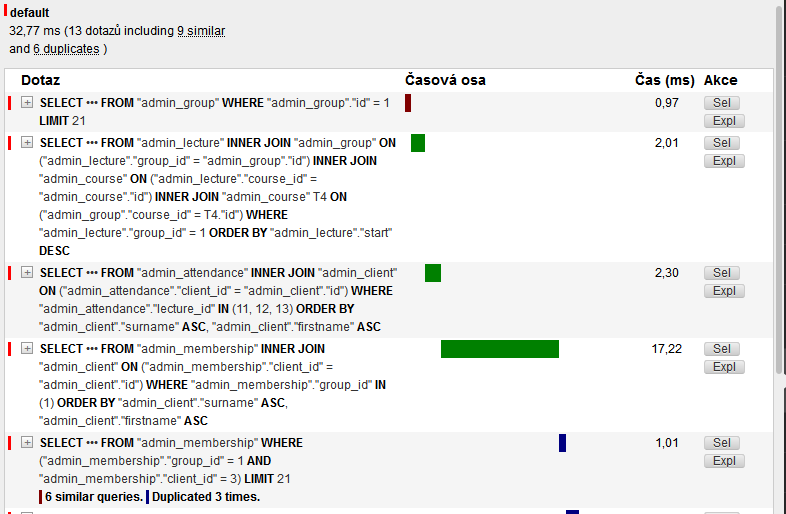
\includegraphics[width=1\textwidth]{img/ddt.png}
    \caption{Analýza SQL požadavku prostřednictvím Django Debug Toolbar}\label{fig:ddt}
\end{figure}

\begin{listing}[ht]
	\begin{minted}[bgcolor=bg]{python}
queryset = (
        Lecture.objects.order_by("-start")
        .select_related("group__course", "course")
        .prefetch_related(
            Prefetch("attendances",
                queryset=Attendance.objects
                    .select_related("client")),
            Prefetch("group__memberships",
                queryset=Membership.objects
                    .select_related("client")),
        ))
	\end{minted}
	\caption{Optimalizace SQL dotazů v Djangu}\label{lst:optimalizace-django}
\end{listing}

V rámci analýzy požadavků také bylo zjištěno, že použitá knihovna pro JWT autentizaci na serverové části (\href{https://github.com/jpadilla/django-rest-framework-jwt}{django-rest-framework-jwt}) nefunguje dle očekávání -- jedním z principů JWT má být, jak bylo uvedeno v rámci bakalářské práce \cite{bp}, že není třeba zatěžovat databázi opakujícími se dotazy, protože všechny potřebné informace jsou součástí objektu tokenu. Knihovna ale při každém přístupu do API stejně kvůli uživateli do databáze přistupovala, tento problém byl hlášen mnoha uživateli \cite{django-rest-framework-jwt-issue}, ale knihovna už není oficiálně udržovaná \cite{django-rest-framework-jwt}. Dle doporučení autora této knihovny byla knihovna nahrazena knihovnou \href{https://github.com/SimpleJWT/django-rest-framework-simplejwt}{django-rest-framework-simplejwt}, byly provedeny příslušné změny pro zmigrování, protože knihovny nemají stejný základ. Díky této migraci už se do databáze opakovaně nepřistupuje. Vzhledem k tomu, že knihovna neposkytuje český překlad, některé notifikace v aplikaci byly v angličtině, proto jsem do projektu přispěl formou PR\footnote{\url{https://github.com/SimpleJWT/django-rest-framework-simplejwt/pull/188}} a kompletní český překlad je již součástí hlavní větve projektu.

Na klientské části bylo identifikováno několik možných vylepšení -- zrychlení vykreslování, rozdělení kódu aplikace na více částí a snížení počtu požadavků na API díky zavedení React Context API.

V původní verzi aplikace se při otevření aplikace v prohlížeči načtou skripty pro celou aplikaci, to je zbytečné, stačí načíst jen ty potřebné pro zobrazení dotyčné stránky, další skripty pak načíst až při přechodu na jinou stránku. Toto chování nově umožňuje React~16.6 pomocí funkce \verb|React.lazy()| a komponenty \verb|Suspense| (ta umožní počkat na lazy načtení importu a mezitím uživateli ukázat zvolenou formu načítání) \cite{react-blog-166}, použití je vidět v ukázce kódu~\ref{lst:optimalizace-react} -- ukázka obsahuje nejdůležitější části kódu z aplikace, tedy použití lazy načtené komponenty \verb|Diary| a zobrazení načítání pomocí \verb|Suspense|. Jak je vidět v kódu, v \verb|React.lazy| se navíc volá ještě funkce \verb|lazySafe|, toto není knihovní funkce, ale přímo mnou implementovaná funkce, která řeší problém, na který se přišlo až několik měsíců po nasazení lazy načítání. Pro pochopení je důležité vědět, že si prohlížeče ukládají do cache kódy aplikace, včetně souboru \verb|manifest.json|, který označuje jednotlivé části kódu aplikace (\enquote{chunky}), jejichž jména jsou hashe dle obsahu souboru. Při nasazení nové verze aplikace se může stát, že lektorka má u sebe starou verzi tohoto souboru a v případě, že došlo ke změně názvů souborů (změna hashe), dojde k chybě \enquote{Error: Loading chunk <číslo\_chunku> failed.}. Toto React prozatím nijak neošetřuje a bylo třeba toto ošetřit tedy přímo ručně -- funkce \verb|lazySafe| monitoruje výskyt zmíněné chyby a pokud nastane, pokusí se znovu načíst celou aplikaci (aby se odstranily staré hashe v cache), ale pouze jednou, aby nedošlo k zacyklení. Díky tomuto ošetření už lektorka neskončí na chybové stránce, ale aplikace se sama zotaví.

\begin{listing}[ht]
	\begin{minted}[bgcolor=bg]{js}
// lazy nacitani pro jednotlive stranky
...
const Diary = React.lazy(
    () => lazySafe(() => import("./pages/Diary")))
...
const Main: React.FC = () => {
    ...
    return (
    ...
    <React.Suspense fallback={<Loading />}>
        ...
        <PrivateRoute
            path={`\${APP_URLS.diar.url}/:year?/:month?/:day?`}
            component={Diary}
        />
        ...
    </React.Suspense>
    )}
	\end{minted}
	\caption{Dělení kódu klientské části v Reactu}\label{lst:optimalizace-react}
\end{listing}

Dalším důležitým vylepšením je zavedení React Context API pro snížení počtu požadavků na API. Context přišel do Reactu v rámci verze~16.3, která vyšla v době dokončení bakalářské práce, umožňuje sdílet data mezi komponentami bez nutnosti explicitního předávání těchto dat skrze \enquote{props} -- tedy dat, která jsou v jistém smyslu globální pro určitý strom komponent \cite{react-context}. Vzhledem k délce kódu souvisejících i se základnějším použitím Context v rámci aplikace uvedu spíše jen základní popis stavebních kamenů Context API -- jsou 3 \cite{react-context}:
\begin{itemize}
    \item \textbf{React.createContext:} funkce vytvářející objekt kontextu,
    \item \textbf{Context.Provider:} komponenta (součást objektu kontextu) umožňující konzumujícím komponentám v daném stromu komponent přihlásit se k odběru změn v kontextu,
    \item \textbf{Context.Consumer:} komponenta (součást objektu kontextu) přihlašující se ke změnám v kontextu.
\end{itemize}

V rámci aplikace byl Context zaveden pro mnoho částí aplikace -- přihlašování/odhlašování (\verb|AuthContext|), aktivní klienti (\verb|ClientsActiveContext|), viditelné kurzy (\verb|CoursesVisibleContext|), aktivní skupiny (\verb|GroupsActiveContext|) a stavy účasti (\verb|AttendanceStatesContext|). Součástí objektů těchto kontextů jsou kromě samotných příslušných dat i metody pro aktualizaci dat, zjištění, zda se data zrovna načítají, zda jsou načtená. Díky tomu lze napříč aplikací získat například stavy účasti bez jakéhokoliv požadavku na API -- data jsou do kontextu načtena při prvním požadavku na data a při úpravě dat (např. přidání klienta) dojde k aktualizaci dat i v kontextu, tedy data jsou stále aktuální. Díky tomu také během přechodů aplikace není třeba na nic čekat a data jsou okamžitě bez načítání zobrazena (některá data, např. neaktivní klienti, v kontextu nejsou, protože je to zbytečné, tedy se stále načítají pokaždé čerstvě). Aplikace je tak svižnější, lektorka nemusí často čekat, API je méně vytížené a tento jednotný přístup umožňuje také lépe kontrolovat, zda se data načítají či nikoliv (to bylo třeba v rámci problému s použitelností~\ref{P11}). Časté požadavky na API plynuly právě z toho, že se přechází např. mezi stránkami v aplikaci a zde nebyla možnost sdílet již načtené stavy účasti, protože se jedná o jiný strom komponent, tedy byly načítány znovu, znovu a znovu.

Dalším drobným vylepšením z hlediska výkonu klientské části při vykreslování a překreslování aplikace bylo odstranění definice komponent z metod \verb|render|, protože komponenty (zejména ty vnořené) se pak musejí při každém vykreslení překreslit všechny, což je zbytečné.

\section{Další řešené problémy}\label{sec:dalsireseneproblemy}

V rámci iteračního vývoje byly řešeny i další různé problémy a vylepšení, které nebyly uvedeny v původních požadavcích. Příkladem budiž implementace drobných změn mimo požadavky uvedených v návrhu datového modelu v sekci~\ref{sec:datovymodel} a komunikačního rozhraní v sekci~\ref{sec:komunikacnirozhrani}. Dále byl zaveden nástroj Google Analytics pro analýzu průchodů aplikací díky knihovně \href{https://github.com/react-ga/react-ga}{react-ga}. V rámci požadavku~\ref{N5} na vylepšení použitelnosti bylo třeba aplikaci při vývoji testovat přímo v mobilním zařízení/tabletu, bylo tedy třeba zprovoznit tuto možnost testování v rámci lokální sítě z jakéhokoliv zařízení (to nebylo v původní aplikaci možné a bylo třeba vždy aplikaci nasadit).

\subsection{Migrace a refaktoring}
V rámci migrace na API nového Reactu~16.3 a dále (která byla plánována již v bakalářské práci \cite{bp}, také toto souvisí s požadavkem na aktualizaci závislostí~\ref{B1}) bylo třeba napříč aplikací provést příslušné změny. Kromě samotného zavedení používání Context API pro optimalizaci práce s API (viz podsekce~\ref{subsec:N6implementace}) bylo třeba přejít na nový životní cyklus komponent Reactu. V rámci této migrace a po ní bylo zjištěno, že se na mnoho místech naprosto zbytečně komplikovaly komponenty metodami jako \verb|getDerivedStateFromProps|, které ale nebyly potřeba (nebylo třeba kopírovat \enquote{props} do \enquote{state}, stačilo číst přímo \enquote{props}), to mohlo také způsobit nečekané problémy a chyby v aplikaci -- při vydání Reactu~16.4 dokonce vychází článek \cite{react-blog-derivedstate} upozorňující právě na mnohdy zbytečné používání těchto metod a možný výskyt chyb. Vzhledem k tomu bylo třeba kompletní klientskou část aplikace projít a vyhledat všechny tyto problémy způsobené faktem, že se v době tvorby původní aplikace toto z důvodu neznalosti používalo. Příkladem reálného příkladu chyby budiž problém s komponentou zobrazující stav účasti klienta na lekci (formou rozbalovacího seznamu) \verb|SelectAttendanceState| -- při změnách architektury Reactu na nástroj nwb a především zavedení \enquote{lazy} načítání v rámci aplikace (v podsekci~\ref{subsec:N6implementace}) se začal projevovat problém se zobrazováním špatného stavu účasti v závislosti na pořadí obdržení odpovědí ze serveru (z API).

Se zmíněnou migrací souvisí i kompletní refaktoring celé klientské i serverové části, zjednodušení a zefektivnění kódu, struktury projektu a souborů, rozdělení do více metod, funkcí, odstranění podobných kódů či nepoužívaných metod (např. díky nástroji \href{https://github.com/jendrikseipp/vulture/}{vulture} pro Python). Na klientské části opravy nekonzistentních stavů (množina možných hodnot ukládaných do stavu byla širší, než měla být),  rozdělené CSS stylů ke komponentám, rozdělení do více komponent, opravy nevalidního HTML a CSS (díky tomu drobné opravy UI), zavedení minifikace HTML, zjednodušení rozhraní komponent. Zmíněný refaktoring měl velký dopad na serverovou část s API, kde byl kód velmi nepřehledný, dlouhý. Tyto velké změny ale bylo samozřejmě možné provádět až při zavedení všech testů pro zásadní části aplikace (viz následující kapitola~\ref{chap:testovani}, aby bylo zajištěno, že tyto změny způsobí co možná nejméně problémů.

V Reactu~16.8 přibyla také možnost používat takzvané \enquote{hooks} -- funkce, které umožňují používat mnoho vlastností Reactu bez tříd a také přepoužívat jednoduše stavovou logiku (bez změny hierarchie komponent, což doteď nebylo možné) \cite{react-docs-hooks}. Jak též článek \cite{react-docs-hooks} uvádí, není třeba hromadně migrovat všechny třídy na klasické funkcionální komponenty s hooky, ale postupně je v dalších iteracích začleňovat při práci na aplikaci -- toho jsem se držel a hooky tak jsou zavedeny pro všechny modální okna (hook \verb|useModal|), také je vytvořen hook pro odchytávání stisku klávesy a práci s daty formuláře. Díky tomu bylo možné v rámci jednoduchých komponent umožnit používání stavu a také dodat mnoho logiky ke stavu navíc -- v případě modálních oken má totiž hook na starost i zobrazování upozornění na ztrátu dat formuláře či třeba předávání dat rodičovským komponentám po odeslání formuláře. Použité jednoduchého hooku pro přidání stavu do funkcionální komponenty je v ukázce~\ref{lst:hook}.

\begin{listing}[ht]
	\begin{minted}[bgcolor=bg]{js}
const [loadingState, setLoadingState] = React.useState(
    LOADING_STATE.NORMAL_LOADING)

React.useEffect(() => {
    const timeoutId = setLoadingTimeout(
        LOADING_STATE.LONG_LOADING)
    return (): void => window.clearTimeout(timeoutId)
}, [])
	\end{minted}
	\caption{Ukázka použití hooků ze souboru Loading.tsx}\label{lst:hook}
\end{listing}

\subsection{Další opravy chyb a vylepšení}

Kromě všech již zmíněných chyb bylo nalezeno množství dalších, pro zajímavost jich několik uvedu v tomto odstavci. V diáři se špatně pracovalo s datem a pokud se do URL zadal datum s 31.~dnem v měsíci, došlo k \enquote{přesunu do minulosti} (číslo dne se změnilo na \enquote{1}) -- v důsledku toho se v aplikaci nedalo dostat do roku 2019, protože 31.~12~2018 bylo pondělí a další týden se přepnul na listopad. Také docházelo k nekorektnímu zobrazení lekcí v předchozím dnu -- pokud by lekce byla v 1~h ráno (což je sice nereálné, ale např. v rámci testů možné), v diáři se ukázala v předchozím dni jako poslední, dělo se to z důvodu porovnávání data s časovou zónou s datem bez časové zóny (vyřešeno použitím \verb|__date| v querysetu na straně API). Dále, při aktualizaci lekce v diáři v rámci nějakého dne došlo pouze k aktualizaci lekcí v rámci daného dnu, neprojevily se změny do jiných dnů (např. informace o \enquote{příště platit}). V souvislosti s výpočtem platby příště docházelo k nekorektním upozorněním, protože logika výpočtu nebrala v úvahu předplacené lekce.

V rámci iteračního vývoje byla vylepšována také stávající implementace nových požadavků, např. bylo potřeba dodat do zájemců o kurzy telefonní číslo klienta, protože bylo zjištěno, že lektorka často tento údaj při práci se zájemcem potřebuje a musí kvůli tomu do karty klienta. Dále bylo napříč aplikací potřeba zvýraznit neaktivitu skupin a klientů -- tedy např. v kartě klienta/skupiny zobrazit upozornění na neaktivitu klientů/skupin/členů skupiny, v seznamu skupin zobrazit upozornění na neaktivního člena apod. -- aby lektorka ihned věděla, že jí vzhledem k uvedené mohou čekat omezení z hlediska funkcí (na základě omezení a validací v sekci~\ref{sec:datovymodel}).

\subsection{Nástroj pro vývoj klientské části}

Jak je popsáno v podsekci~\ref{subsec:bp-klientskacast}, původní verze aplikace z bakalářské práce je založena na nástroji \href{https://github.com/facebook/create-react-app}{create-react-app~1}, vzhledem k tomu, že bylo třeba propojit pro vývoj klientskou část s Djangem, bylo třeba provést \enquote{eject}, tedy prakticky všechny konfigurační soubory ad. budou k dispozici, není ale cesty zpět. Pro rozjezd projektu to bylo důležité, protože pak stačilo konfiguraci upravit ku obrazu svému. Problém ale nastává z hlediska dlouhodobé udržovatelnosti klientské části, protože při každé aktualizaci Reactu (nebo nástroje create-react-app) je potřeba vše znovu přegenerovat a ručně porovnat konfigurace a na příslušné řádky opět dodat potřebné skripty. To je samozřejmě neudržitelné. Z toho důvodu byly hledány alternativy, byly 2 možnosti. Použít nástroj pro klientskou část, který umožní konfiguraci příslušných částí a zároveň jednoduchou aktualizaci (tedy prakticky nástroj, který zaobalí všechny potřebné nástroje pro vývoj a jednoduše umožní bez hlubokých znalostí vše potřebné nakonfigurovat). Nebo všechny nástroje a závislosti nakonfigurovat a spravovat po svém. V květnu 2019 byla tedy zvolena první varianta jiného nástroje a k tomu byl nalezen nástroj \href{https://github.com/insin/nwb}{nwb} -- který byl do té doby dobře spravovaný a aktualizovaný a populární (poslední aktualizace proběhla v březnu 2019) a nabízel vše potřebné.

Zmíněná poslední aktualizace byla ale poslední doslova, postupem času se začaly kupit problémy týkající se optimalizace klientské části a bezpečnosti (mnoho z aktuálních požadavků v rámci této práce také, např. \enquote{lazy} načítání, CSP ad.), které všechny čekaly na vyřešení různých problémů v tomto nástroji, které ale řešeny nebyly a autor přestal reagovat. V únoru 2020 tak bylo třeba přistoupit na změnu, opět byly 2 možné cesty -- zvolit nový nástroj a nebo vše nakonfigurovat ručně. Jako možný nový nástroj se ukázal nástroj \href{https://github.com/neutrinojs/neutrino/}{Neutrino}. Bylo rozhodnuto, že se provede testovací migrace jak na Neutrino, tak na vlastní konfiguraci všech nástrojů bez jakékoliv nadstavby v podobě abstrakce nad všemi nástroji (jako třeba Neutrino či nwb). Výsledkem byly nakonec tři finální verze ve třech větvích repozitáře -- vlastní konfigurace, Neutrino a nejnovější verze nástroje nwb (tento nástroj jen pro referenci a srovnávání). První dva nástroje byly porovnávány jak z hlediska fungování, výstupního kódu klientské části po sestavení (především jeho velikosti) a z hlediska jednoduchosti rozšiřování konfigurace. Postupnými změnami konfigurace (nástrojů Webpack, Babel a mnoha dalších) bylo dosaženo stavu, kdy výstupy sestavené klientské části byly prakticky totožné (i velikostí), tedy nikde nebylo ve vlastní konfiguraci opomenuto nic podstatného oproti nástrojům jako nwb či Neutrino. Abstraktní vrstva nad nástroji, kterou nabízí Neutrino, nabízí výhodu v podobě zdánlivě jednoduché konfigurovatelnosti, to je ale za cenu toho, že je třeba podrobně studovat dokumentaci a složitě nalézat, jakou jednoduchou cestou provést nějakou konfiguraci. Naproti tomu totéž v případě vlastní konfigurace je naprosto jednoduché, protože z dokumentace příslušného nástroje (např. Webpack) přesně víme, kde máme co upravit (což v Neutrinu může být naprosto kdekoliv). Tedy, vzhledem k tomu, že jednoduchá konfigurace byla na úkor toho, že je třeba složitě hledat a zkoušet, kam lze napsat kýženou konfiguraci a také vzhledem k tomu, že by se opět záviselo na nástroji, který může být pomalu vyvíjený, bylo rozhodnuto o nezavedení Neutrina (či jiných nástrojů) a o migraci na kompletní vlastní řešení v podobě vlastní konfigurace všech nástrojů a správy závislostí. K tomu bylo třeba podrobně nastudovat příslušné dokumentace, aby byla konfigurace v co nejlepším stavu, výhodou je ale naprostá nezávislost na nadstavbových nástrojích a v případě, že dorazí nějaká novinka, takový nástroj nebude tuto novinku blokovat v její implementaci a začlenění do projektu. V březnu 2020 tak mohlo být toto řešení (dokonce s rovnou začleněným TS) vydáno.

\chapter{Testování}\label{chap:testovani}

V souladu se zvoleným přístupem k testování v sekci~\ref{sec:zvolenetechnologie-testovani} a požadavkem~\ref{N2} byly implementovány v Pythonu API a UI (e2e) testy. Jak zde bylo též uvedeno, bude k tomu využit nástroj behave založený na BDD -- vzhledem k tomu, že v době vytváření testů byla již část aplikace hotová (mírně rozšířená verze oproti bakalářské práci), doslovně zde nelze aplikovat BDD přístup popsaný v podsekci~\ref{subsec:bdd} (protože aplikace je již napsaná), scénáře a testy tedy byly dopsány zpětně, při dalším rozšiřování již mohly být scénáře psány předem.

\section{Scénáře}

Scénáře v prakticky přirozeném jazyce (Gherkin), které popisují požadované chování aplikace -- v jednotlivých krocích (\enquote{steps}). Pro tyto kroky jsou pak implementovány samotné testy, tomu se budu věnovat v následující sekci. Scénáře mohou být psány v mnoha jazycích, pro jednoduchost a srozumitelnost byla zvolena výchozí angličtina. Funkcionality (\enquote{features}) se pak sestávají z více různých scénářů chování aplikace pro danou funkcionalitu, jeden ze scénářů pro funkcionalitu klientů (ze souboru \verb|clients.feature|) je vidět v ukázce kódu~\ref{lst:gherkin}. Kromě samotného scénáře je zde vidět použití tagů (pomocí \enquote{@}), díky tomu lze pak jednoduše selektivně spouštět např. pouze testy pro mazání či pro klienty apod. Mnoho ze scénářů je ale mnohem složitějších a používají klíčová slova \verb|Scenario Outline|, díky kterým lze spouštět daný scénář s různými kombinacemi hodnot (v reálu např. různé údaje klientů). Tyto soubory jsou ve složce \verb|tests/features|.

Při psaní scénářů, jak bylo uvedeno v sekci~\ref{sec:zvolenetechnologie-testovani}, byly scénáře vytvářeny na základě reálných požadavků a nejdůležitějších funkcionalit a vlastností aplikace. Výsledkem je 7 funkcionalit (stavy účasti, zájemci o kurzy, klienti, kurzy, skupiny, lekce, přihlášení/odhlášení), sestávajících se z celkem 94 scénářů, scénáře se celkem skládají ze 374 kroků (to ale neznamená, že bude naimplementováno 374~metod pro testování, bude jich méně, protože mnoho z nich využívá opakovaně též kroky díky již zmíněnému \verb|Scenario Outline|).

\begin{listing}[ht]
	\begin{minted}[bgcolor=bg]{gherkin}
Feature: Operations with clients
    Background: Prepared database and logged user
        Given the database with some clients
        And the logged user
        
    @delete @clients
    Scenario: Delete client
        When user deletes the client "Rod Lukáš"
        Then the client is deleted
	\end{minted}
	\caption{Ukázka scénáře pro smazání klienta v souboru clients.feature}\label{lst:gherkin}
\end{listing}

\section{Implementace testů}

Samotné implementace testů spouští behave na základě scénářů z předchozí sekce, každý krok scénáře příslušní dané implementaci v kódu. Vzhledem k tomu, že se testuje API a UI, tedy dvě vrstvy, bylo třeba tyto testy držet od sebe oddělené -- aby jediné, co mají společné, je implementace kroků ze scénářů (souborů \verb|*.feature|). Bylo zde zavedeno dělení, které behave umožňuje -- kroky UI a API jsou v separátních složkách \verb|api_steps| a \verb|ui_steps|. Dále je zavedena složka \verb|common_steps|, která obsahuje společné testovací kroky pro obě části, které zařídí připravenou a naplněnou databázi daty, které vychází z připravených dat v rámci souboru \verb|fixtures.py|.

V ukázce kódu~\ref{lst:behave-implementace} je implementovaný krok ověřující úspěšné smazání klienta, konkrétně pro část API. Testy API, jak bylo uvedeno v sekci~\ref{sec:zvolenetechnologie-testovani} jsou méně křehké a více stabilní oproti UI, jsou také mnohem jednodušší, protože jsou pouze založené na modelu požadavek a odpověď, kdežto testování UI je mnohem komplexnější.

Jedním z cílů bylo, aby i přes větší křehkost UI testů byl kladen důraz na to, aby výsledná křehkost byla co nejnižší. Pro představu, pokud bychom ve stávající klientské části přistupovali přesně ke každému elementu a jeho obsahu bez jakéhokoliv přemýšlení, můžeme díky zápisu XPath (který Selenium používá) získat kód velmi závislý na konkrétním UI kvůli explicitně uvedené cestě k elementu. Pokud místo toho budeme v rámci aplikace při testování přistupovat k obsahu elementu pomocí jiného mechanismu nezávislého na konkrétní implementaci, stabilita testů by byla mnohem vyšší -- tento mechanismus je známý a používá se v rámci Selenium komunity \cite{dataqa}, využívá vlastního HTML atributu s názvem obvykle \verb|data-qa|, který obsahuje příslušný název obsahu, implementovaný test pak nepřistupuje k elementu v závislosti na aktuální podobě UI, ale pouze pomocí selektoru najde ve stránce příslušný element s názvem v tomto atributu, viz ukázka kódu~\ref{lst:behave-implementace2}. Pokud tedy nedojde ke změnám v oblasti logiky aplikace, ale pouze se určitý element přesune ve struktuře HTML do jiného uzlu, pokud mu ponecháme tento atribut, testy nadále fungují a není třeba je nijak upravovat a jsou tak mnohem stabilnější. Pro některé knihovny UI (např. react-select) dodání vlastního atributu není možné, proto používají atributy \verb|id| nebo \verb|class|.

\begin{listing}[ht]
	\begin{minted}[bgcolor=bg]{python}
@then("the client is deleted")
def step_impl(context):
    assert context.resp.status_code == 
        status.HTTP_204_NO_CONTENT
    assert not helpers.find_client_with_full_name(
        context.api_client, context.full_name)
    assert clients_cnt(context.api_client) < 
        context.old_clients_cnt
	\end{minted}
	\caption{Implementace kroku ověřujícího, že je klient smazaný -- ze souboru api/clients.py}\label{lst:behave-implementace}
\end{listing}

\begin{listing}[ht]
	\begin{minted}[bgcolor=bg]{python}
surname_field = context.browser.find_element_by_css_selector(
    "[data-qa=client_field_surname]")
	\end{minted}
	\caption{Přístup k elementům v UI nezávislý na konkrétní implementaci UI}\label{lst:behave-implementace2}
\end{listing}

Pro integraci behave s Django se používá knihovna \href{https://github.com/behave/behave-django}{behave-django}. Pro Selenium se používá pro integraci s prohlížečem webdriver \href{https://github.com/mozilla/geckodriver}{geckodriver}, ten umožňuje Seleniu interagovat s prohlížečem Firefox, toto je zvoleno právě na základě primárního prohlížeče používaného lektorkou. Firefox je pak možné používat jak v rychlejším \enquote{headless} módu bez GUI, nebo pomalejším běžném režimu, kdy je možné sledovat průchody UI aplikace při testu.

Při implementaci UI testů se objevilo několik problémů, v prvé řadě muselo být kompletně upraveno napříč aplikací načítání (součást problému s použitelností~\ref{P11}), protože skripty potřebují vědět, kdy se mohou začít rozhlížet po stránce a v ní obsažených datech. Toto bylo napříč aplikací opraveno a díky testům tak víme, že je lektorka informována o načítání skutečně vždy (v testovaných případech) korektně. Dále během vývoje v iteracích nastalo několik situací, kdy se testy ukázaly slabé. Například při pokusu o úpravu stávajících dat nekontrolovaly, zda jsou stávající data ve formuláři zobrazena korektně (což umožnilo vznik chyby v souvislosti se špatným zobrazením doby trvání kurzu). Dále v rámci úprav formuláře pro lekce byl hlášen problém ohledně tlačítka pro přidání lekce, které nebylo aktivní a lekci tak nešlo uložit, napříč tomu, že testy procházely (protože používaly pro odeslání formuláře stisk ENTER, reálné chování uživatele je ale obvykle stisk tlačítka pro odeslání). Během testování se náhodně objevovaly nefunkční testy, zde se jednalo o falešně pozitivní hlášení, protože aplikace fungovala korektně -- nastal zde ale problém s localStorage, kdy uložené údaje (JWT token) se nestihly pro další scénář smazat, po každém scénáři tak behave automaticky localStorage smaže. UI testy byly také zpočátku poměrně pomalé, podrobnější inspekcí bylo zjištěno, že se v určitých krocích zbytečně dlouho čeká, toto bylo opraveno.

Dalším problémem při práci se Seleniem byla dokumentace jeho API pro konkrétní jazyk, která byla v případě Pythonu poměrně nepřehledná, navíc někdy odlišná od API pro Selenium v Javě, kde se vyskytovalo více možností oproti Pythonu.

Pro všechny důležité části aplikace jsou testy naimplementovány, napsané scénáře také slouží jako dokumentace, čehož bylo s úspěchem využito při práci na tvorbě testů v rámci předmětu \textit{MI-PYT}, kde vyučující mohl jednoduše vidět, co je testováno za funkce a jaké je pokrytí. Co se týče percentuálního pokrytí kódu testy, je cca 84~\%, toto číslo ale nemá příliš vypovídající hodnotu a důležitější je tak fakt, že jsou pokryty všechny důležité průchody v aplikaci. Paralelně k tomu je zároveň veden seznam zbývajících průchodů (soubor \verb|tests/MANUAL_TESTS.md|), které nejsou pokryty automatizovanými testy.

\subsection{Další testování}

Automatizované testování je možné spouštět jak na lokálním stroji, tak i na CI -- tomu se budu věnovat v následující kapitole~\ref{chap:nasazeni}.

Automatizované testy nejsou ale jedinou formou testování v projektu. Samozřejmostí je také akceptační testování v rámci iterací při zavádění různých požadavků. Dále je též při větších změnách prováděno manuální testování zbylých průchodů v aplikaci, které nejsou automatizovány, toto se vyplatí, protože se nejedná o průchody nejdůležitější a velké změny se nedějí často (naopak by se nevyplatilo automatizovat úplně vše, viz podsekce~\ref{subsec:testingpyramid}).

\chapter{Nasazení}\label{chap:nasazeni}

V této kapitole popíši nový způsob řešení nasazování aplikace do více prostředí (viz požadavek~\ref{N7}) další související, jako například zavedení pravidelných záloh databáze z produkce (viz požadavek~\ref{N8}).

\section{Aktualizace prostředí a vylepšení}

Před provedením samotných změn týkajících se nasazení do více prostředí bylo třeba provést aktualizace prostředí na integračním serveru a další změny. V původní verzi aplikace byl Travis nakonfigurován pro původní verze Node.js, PostgreSQL a Python -- zde bylo potřeba vše zmigrovat na verze nejnovější v souladu s aplikací, pro PostgreSQL bylo třeba učinit pokročilejší konfiguraci, protože Travis zatím nepodporuje jednoduchý výběr nejnovějších verzí PostgreSQL. Aby bylo možné používat novější Python, bylo třeba přejít na nový obraz systému \enquote{bionic}.

Pro Pipenv (na který bylo na Travisu také třeba zmigrovat z pip) a Yarn bylo třeba zavést cache, protože jinak trvalo sestavení aplikace na CI velmi dlouho. V rámci zavedení proměnných prostředí konfigurovaných z Djanga (v rámci požadavku~\ref{N4}, konkrétně problému~\ref{B5}, k implementaci došlo v podsekci~\ref{subsec:N4implementace}) bylo toto třeba taktéž přizpůsobit a nakonfigurovat v Travisu. Pro správné fungování českého jazyka při řazení v databázi bylo třeba stáhnout na Travisu příslušné balíčky. Toto i další operace jsou nově ve zvláštních skriptech ve složce \verb|scripts|, rozdělené dle toho, zda se používají jen na Travisu, na Heroku, nebo na obou platformách.

Součástí zmíněných spouštěných skriptů je nově například také skript pro substituci řetězců napříč celou aplikací (tedy klientskou i serverovou částí). Ukázalo se, že je totiž potřeba v aplikaci spravovat několik řetězců na obou těchto částech a mít jednotnou možnost jejich přizpůsobení -- bylo by totiž samozřejmě možné např. dodat token pro Sentry do Pythonu z prostředí, ale jelikož klientská část je sestavená ze statických souborů, které nemají přístup k proměnným prostředí, nemohla by tímto způsobem klientská část k danému tokenu přistoupit. Dalším příkladem jsou informace o verzi aplikace, větvi, commitu ad., které jsou k vidění v nastavení aplikace a používají se také pro další nástroje, aby tyto měly k dispozici informaci o aplikaci (např. Sentry). V ukázce kódu~\ref{lst:envjs} je vidět způsob řešení dvou řetězců, Travis tyto řetězce pak nahradí příslušnými hodnotami z proměnných prostředí (pro soubory klientské i serverové části).

\begin{listing}[ht]
	\begin{minted}[bgcolor=bg]{ts}
Sentry.init({
    dsn: "\%SENTRY_DSN",
    environment: getEnvName(),
    release: "\%GIT_COMMIT",
})
	\end{minted}
	\caption{Substituce řetězců na Travisu}\label{lst:envjs}
\end{listing}

\section{Testování}

Na Travisu se spouští mnoho testů, nejprve se spustí testy pro typovou kontrolu klientské části (TS) a poté serverové části (mypy). Následně se automaticky nejdříve spustí několik základních smoke testů (složka \verb|admin/tests|) a pakliže vše projde, spustí se nejprve automatizované testy API (které jsou rychlejší a tím pádem rychleji dojde k odhalení případné chyby, která by pravděpodobně ovlivnila i následující UI testy). Poté se spustí i UI testy, které trvají déle, ale výsledkem je zaručení, že důležité části aplikace jsou s nejvyšším pravděpodobností funkční. Výsledné pokrytí se reportuje do služby codecov.

\section{Nasazování na více prostředí}\label{sec:nasazovani-nasazovaninaviceprostredi}

Původní způsob nasazování každé revize na produkční prostředí byl dle návrhu v sekci~\ref{sec:konfiguraceviceprostredi} nahrazen nasazením na prostředí \enquote{testing} pro každý commit z jakékoliv větve a na prostředí \enquote{staging} a produkci při vytvoření release na GitHubu.

V sekci~\ref{sec:prostreditestovaninasazovani} bylo zmíněno, že ačkoliv se všechny kroky sestavení aplikace odehrají na Travisu, totéž se znovu děje na Heroku, ačkoliv to nemá význam, zpomaluje to nasazování a může vyústit v nefunkční sestavení kvůli mnoha různým důvodům. Z toho důvodu bylo Heroku nakonfigurováno tak, aby pouze provedlo migrace databáze a následně aplikaci spustilo díky všem dodaným závislostem nahraným z Travisu. Na Travisu bylo nově zařízeno, aby se zbytečně nenahrávaly na Heroku např. soubory s testy, dokumentací apod., které nejsou potřeba.

Mimo návrh bylo kvůli požadavku na zveřejnění aplikace jako open-source v rámci zadání práce rozhodnuto, že dojde k zavedení ještě jednoho prostředí. Toto prostředí s názvem \enquote{demo} obsahuje demoverzi aplikace, kterou si může kdokoliv vyzkoušet -- přihlašovací údaje budou veřejně dostupné. Aby se zde nehromadily nesmyslná data v databázi, díky doplňku \href{https://devcenter.heroku.com/articles/scheduler}{Heroku Scheduler} dojde každý den v noci k automatickému smazání všech data a nahrání vzorových dat, která ukazují možnosti aplikace. Oproti ostatním prostředím zde nejsou povoleny výpisy z banky. Nasazení nové verze aplikace na prostředí oproti ostatním prostředím nesouvisí s přidáním revize či releasu, je založeno na přístupu zmíněném v sekci~\ref{sec:prostreditestovaninasazovani}, kde je vytvořena příslušná větev demo, do které se vždy pomocí sloučení změn z vývojové větve \verb|master| přidají nové změny -- tento jiný způsob je zvolen kvůli tomu, aby bylo jasně pod kontrolou, která revize je nahraná na tomto prostředí a dostupná přístupná pro veřejnost, protože tato demoverze slouží například i jako ukázka výsledků této práce např. pro oponenta, není tedy možné, aby zde kvůli vydání nové verze proběhly nějaké změny, verze musí zůstat zachovaná, dokud nebude ručně nasazena jiná.

Kromě zmíněných změn bylo na Heroku samozřejmě potřeba zavést korektně všechny proměnné prostředí. Dále pro prostředí \enquote{testing} bylo umožněno spouštění nástroje Django Debug Toolbar (ve výchozím stavu toto není možné, ale prostřednictvím proměnných prostředí lze nástroj aktivovat a umožnit tak profilování aplikace a databáze i na vzdáleném prostředí, nikoliv pouze na prostředí lokálním. Toho bylo při optimalizaci práce s databází v rámci požadavku~\ref{N6} taktéž využito.

Na produkci bylo zavedeno automatické zálohování databáze, Heroku toto umožňuje jednoduše nastavit \cite{heroku-backups}, toto bylo tedy nastaveno a k automatické záloze dojde každý den v nočních hodinách. Zálohy jsou ukládány každý den a zpětně je dostupných vždy 7~záloh pro předchozích 7~dnů a 1 týdenní záloha, ty je možné obnovit. Kompletní výsledná konfigurace Travisu je v souboru \verb|travis.yml| a vzhledem k její rozsáhlosti ji zde neuvádím.

\section{Ukázka aplikace}

V rámci této sekce pro ilustraci uvedu na obrázku~\ref{fig:screen-tyden} jednu ukázku z reálně nasazené aplikace (data jsou fiktivní), konkrétně z diáře -- zde je velmi dobře vidět, jak jsou například nově začleněny barvy kurzů do UI aplikace (viz požadavek~\ref{F12}), je zde vidět mnoho možností zefektivňujících práci v rámci aplikace (např. rychlé přidání lekce pro daný den, pro jiný den, rychlá úprava lekce, rychlý přechod do karty klienta/skupiny přes jméno, viz požadavek~\ref{F11}), vyhledávání v aplikaci (v horní části, viz požadavek~\ref{F4}). Další snímky z obrazovek jsou k dispozici ve veřejně dostupném repozitáři s aplikací zveřejněném v rámci následující kapitoly~\ref{chap:zverejnenijakoopensource}.

\begin{landscape}
    \begin{figure}\centering
    	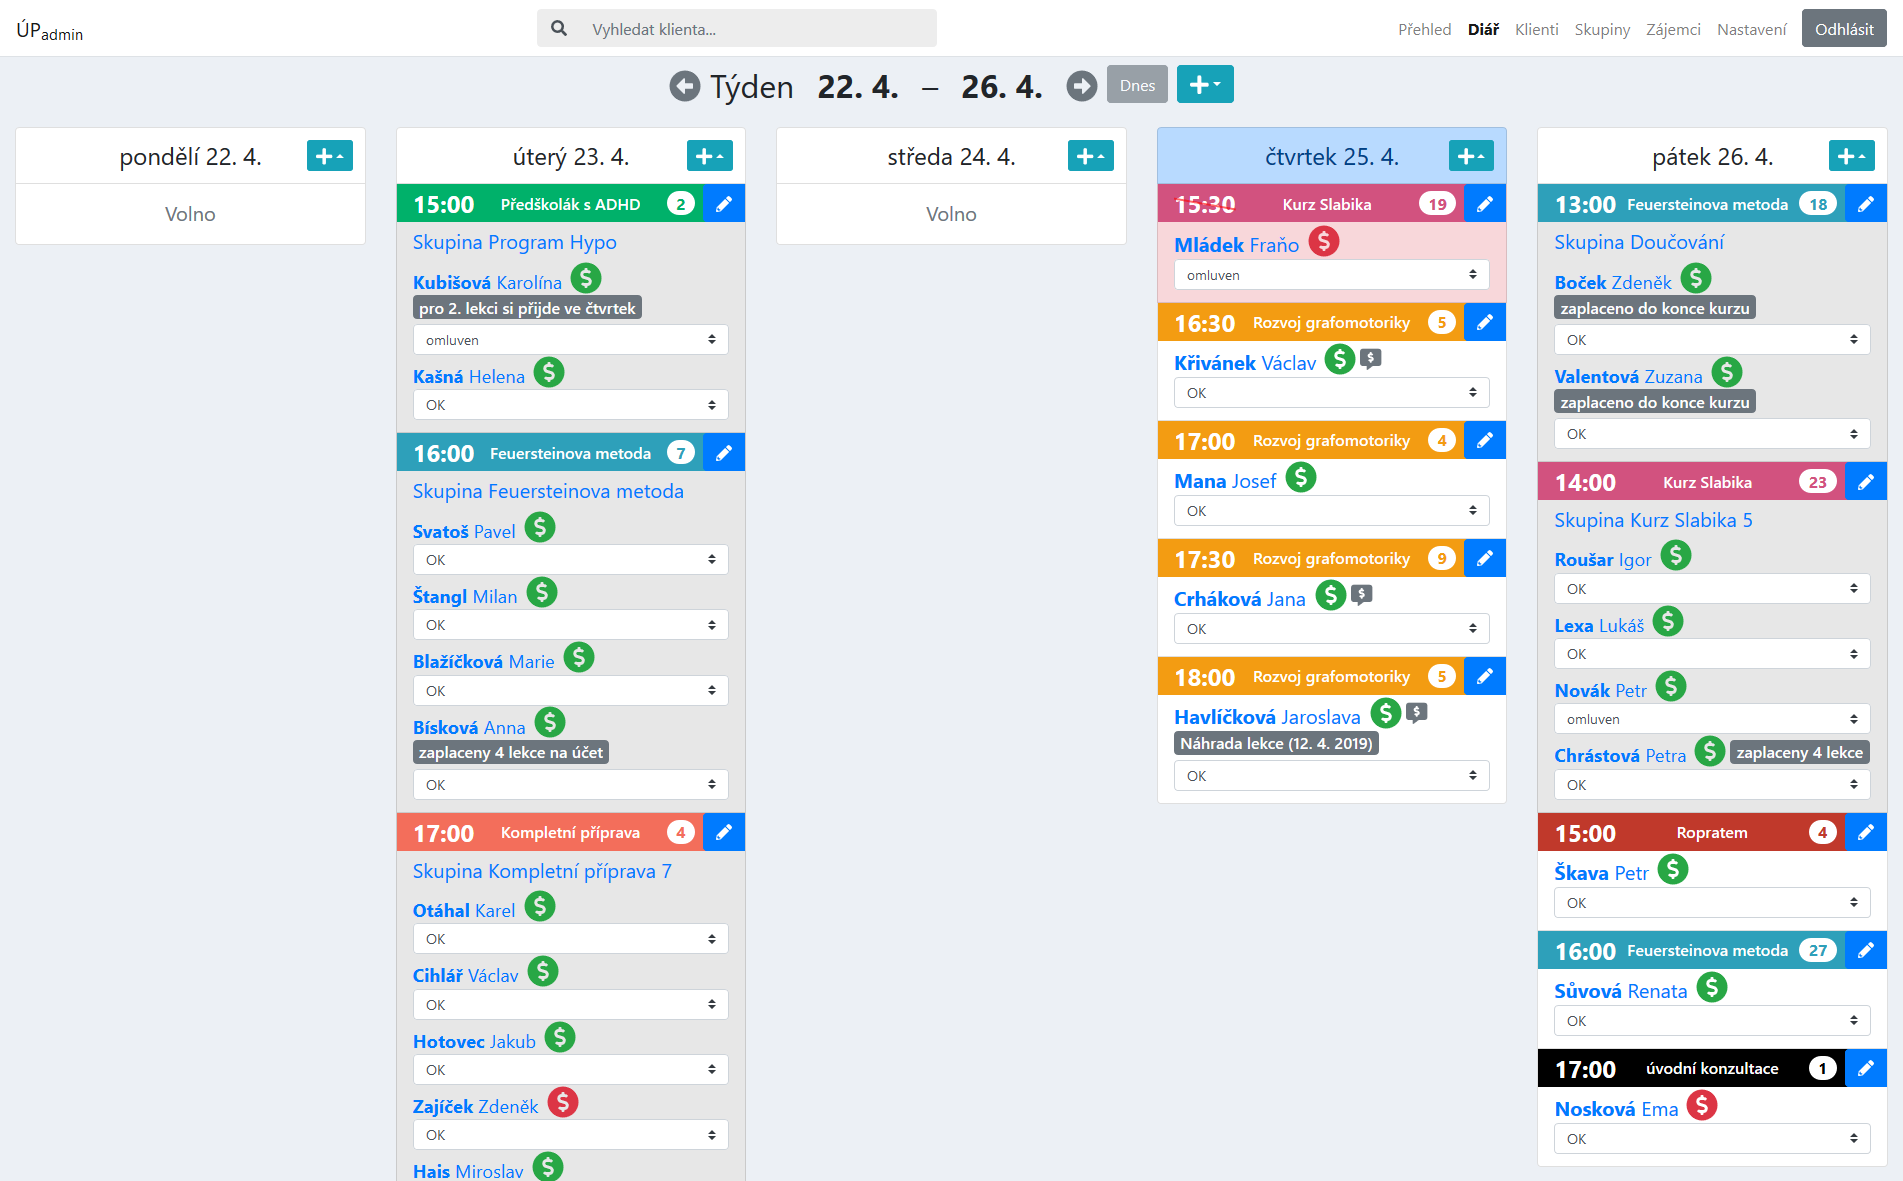
\includegraphics[totalheight=0.83\textheight]{img/diary.png}
    	\caption{Snímek obrazovky s týdenním přehledem}\label{fig:screen-tyden}
    \end{figure}
\end{landscape}

\chapter{Zveřejnění jako open-source}\label{chap:zverejnenijakoopensource}

Jedním z úkolů této práce je její zveřejnění jako open-source. Vzhledem k tomu, že je aplikace vytvořena na míru projektu ÚP, nepočítá se zde, že by snad byla využívána ostatními i v jiných projektech (ačkoliv je toto samozřejmě teoreticky možné). Hlavní pointou zveřejnění je možnost vývojářů nahlédnout na reálnou aplikaci vytvořenou pomocí nejnovější technologií, projít si její konfiguraci, inspirovat se. Taktéž se jedná o mou vlastní referenci.

V rámci příprav na zveřejnění bylo třeba zpřehlednit strukturu repozitáře, zkontrolovat, že neuniknou žádné soukromé přístupové údaje (např. v případě již zmíněného problému s tokenem FontAwesome v problému s bezpečností~\ref{B5} jej bylo třeba přegenerovat, jinak by byl dostupný v historii repozitáře). Dále bylo třeba zvolit vhodnou licenci, zde byla pro svou jednoduchost zvolena licence MIT. Dále bylo třeba doplnit vzorové hodnoty proměnných prostředí do souboru \verb|.env.template| (zde využívám toho, že je již z podsekce~\ref{subsec:N4implementace} připravena právě práce s proměnnými prostředí jakožto konfigurací celé aplikace).

Hlavním problémem, který souvisí se zveřejněním, je využívání privátních npm registrů pro FontAwesome~PRO -- tedy běžný uživatel nemá k dispozici příslušný token a nemůže si sestavit klientskou část. Toto bylo vyřešeno propojením Travis~CI a GitHub tak, že sestavená klientská část z Travisu (který z proměnných prostředí má k dispozici tokeny) se nahraje při releasu k tzv. \enquote{assets} u daného release, viz obrázek \ref{fig:gh}. Tento \verb|zip| soubor obsahuje statické soubory klientské části připravené k servírování jak na produkci, tak při lokálním spuštění dle návodu v repozitáři -- díky tomu, že je již klientská část takto sestavená, není třeba žádných tokenů.

V repozitáři je \verb|README|, které je ve dvou jazycích -- anglickém a českém. Obsahuje informace pro otevření již nasazené demo verze aplikace (viz sekce~\ref{sec:nasazovani-nasazovaninaviceprostredi}) -- zde tedy doporučuji čtenáři tuto stránku\footnote{\url{https://github.com/rodlukas/UP-admin\#demo}} navštívit a demo verzi vyzkoušet. Dále obsahuje základní informace o aplikaci, klíčové funkce, použité technologie a nástroje pro serverovou i klientskou část, informace o nasazených aplikacích a nástrojích, struktuře repozitáře a v neposlední řadě obsahuje také samozřejmě podrobný srozumitelný návod pro spuštění aplikace v lokálním prostředí (včetně minimálních požadavků), práci s testy, licenci a screenshoty z aplikace. V dalších souborech jsou pak dostupné pokročilejší informace o testech či diagramy.

\begin{figure}[h]\centering
    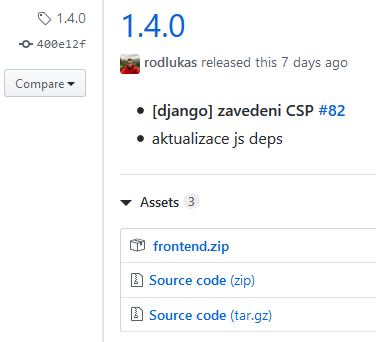
\includegraphics[width=0.6\textwidth]{img/gh.png}
    \caption{Sestavená klientská část ke stažení na GitHubu}\label{fig:gh}
\end{figure}

Repozitář byl úspěšně zveřejněn\footnote{\url{https://github.com/rodlukas/UP-admin}} a obsahuje všechny informace o aplikaci včetně použitých technologií, funkcí, minimálních požadavků, návodů na spuštění, vzorových dat a dalších informací o architektuře a testech.

\chapter{Možná rozšíření}

V rámci této práce byly pokryty implementací funkčních požadavků všechny oblasti aplikace a zatím nejsou známé žádné funkční požadavky do budoucna. Z mého pohledu je možné, že se bude zasahovat do oblasti klientů, kde v aplikaci bude v budoucnu přibývat více a více klientů a lektorka možná bude požadovat jednoduchou možnost mazání velmi starých klientů -- v aktuální podobě lze díky omezením ze sekce~\ref{sec:datovymodel} klienta smazat pouze pokud nemá žádné lekce, toto omezení by bylo třeba v této souvislosti upravit, zmírnit či obcházet.

Z bakalářské práce zůstaly dvě možné oblasti rozšíření vyřazeny (viz podsekce~\ref{subsec:vyrazenepozadavky}) -- evidence pomůcek a učebnic pravděpodobně nebude s aplikací potřeba slučovat, protože postačuje její současné řešení. Offline přístup a SSR je ale oblast, o kterou lze na základě rešerše a prozkoumání možností aplikaci rozšířit.

Co se týče dalších vylepšení klientské části, je zde plánovaná migrace na \verb|PureComponent| a \verb|React.memo| -- to umožní dále optimalizovat výkon klientské části a odstranit další zbytečná překreslování \cite{react-docs-api} (další optimalizace byly již provedeny v rámci implementace požadavku~\ref{N6}, viz podsekce~\ref{subsec:N6implementace}). Dále je plánováno zjednodušení některých rozsáhlých komponent, zejména pomocí \enquote{hooků}, byly zmíněny v sekci~\ref{sec:dalsireseneproblemy}, či rozdělení na více komponent. Výhledově bude také možné v aplikaci použít komponentu \verb|Suspense| (která je již v aplikaci použita pro \enquote{lazy} načítání stránek aplikace, viz podsekce~\ref{subsec:N6implementace}) pro práci s API -- umožnilo by to výrazné zjednodušení a vylepšení práce s API v rámci klientské části, zatím ale tuto komponentu pro toto načítání použít nelze, tato funkcionalita bude až v některé z dalších verzí Reactu~\cite{react-blog-roadmap}. S úpravou načítání také souvisí možnost přidání tlačítka pro obnovení dat v aplikaci bez překreslení celé aplikace (to by totiž udělalo nativní tlačítko v prohlížeči). Dalším možným rozšířením Reactu, které prozatím nebylo možné začlenit kvůli knihovnám, které používají zastaralé API Reactu, je použití komponenty \verb|StrictMode| -- ta umožní ve vývojovém režimu upozornit na používání zastaralého API Reactu a také může pomoci při zachycení některých chyb v kódu související s vedlejšími efekty při překreslování \cite{react-docs-strictmode}.

Co se týče dokumentace, je v plánu doplnění dokumentace do kódu pro metody v komponentách klientské části a dále upřesnění typových anotací parametrů na serverové části, kde je např. očekáván obecný slovník, ale je vhodnější zavést striktnější kontrolu obsahu slovníku. Další možnou oblastí je zavedení kontejnerizace (např. Docker), to by mohlo usnadnit např. práci s databází.

Všechna zmíněná možná vylepšení jsou evidována v \enquote{issues} v GitHub repozitáři\footnote{\url{https://github.com/rodlukas/UP-admin/issues}} (který byl zveřejněn v rámci kapitoly \ref{chap:zverejnenijakoopensource}).
